%
% equation and figure referencing to do
% 
\documentclass[twoside,a4paper,11pt]{report}

\usepackage{amsmath}
\usepackage{amssymb}
\usepackage{graphicx}
%\usepackage[thmmarks]{ntheorem}
\usepackage{theorem}
\usepackage{fancybox}
\usepackage{subfigure,wrapfig}
\usepackage{bm}

\usepackage{fancyheadings}
\pagestyle{fancyplain}

\renewcommand{\chaptermark}[1]
{\markboth{#1}{}}
\renewcommand{\sectionmark}[1]
{\markright{\thesection\  #1}}
\lhead[\fancyplain{}{\bfseries\thepage}]
{\fancyplain{}{\bfseries\rightmark}}
\rhead[\fancyplain{}{\bfseries\leftmark}]
{\fancyplain{}{\bfseries\thepage}}

\cfoot{}

\newcommand{\Tf}[2]{\textstyle\frac{#1}{#2}}

{\theoremstyle{plain} 
\newtheorem{exmp}{Example}}

{\theoremstyle{plain} 
\newtheorem{Def}{Definition}}

{\theoremstyle{plain} 
\newtheorem{Rem}{Remark}}

{\theoremstyle{plain} 
\newtheorem{exercise}{Exercise}}

\newcommand{\rbegin}[1]{\bigskip \hrule\begin{#1}}
\newcommand{\rend}[1]{\end{#1} \hrule\bigskip}

{\theoremstyle{plain} \newtheorem{theorem}{Theorem}
%
\begin{document}

\pagenumbering{roman}

\title{{
\includegraphics[width=2.5in]{mlogo.pdf}}\\
\large{School of Mathematical Sciences}\\
\vfill
\Huge{MTH3360 --- Fluid Mechanics}\\
\Huge{Part 2: Incompressible Fluids}\\
\bigskip
\bigskip
{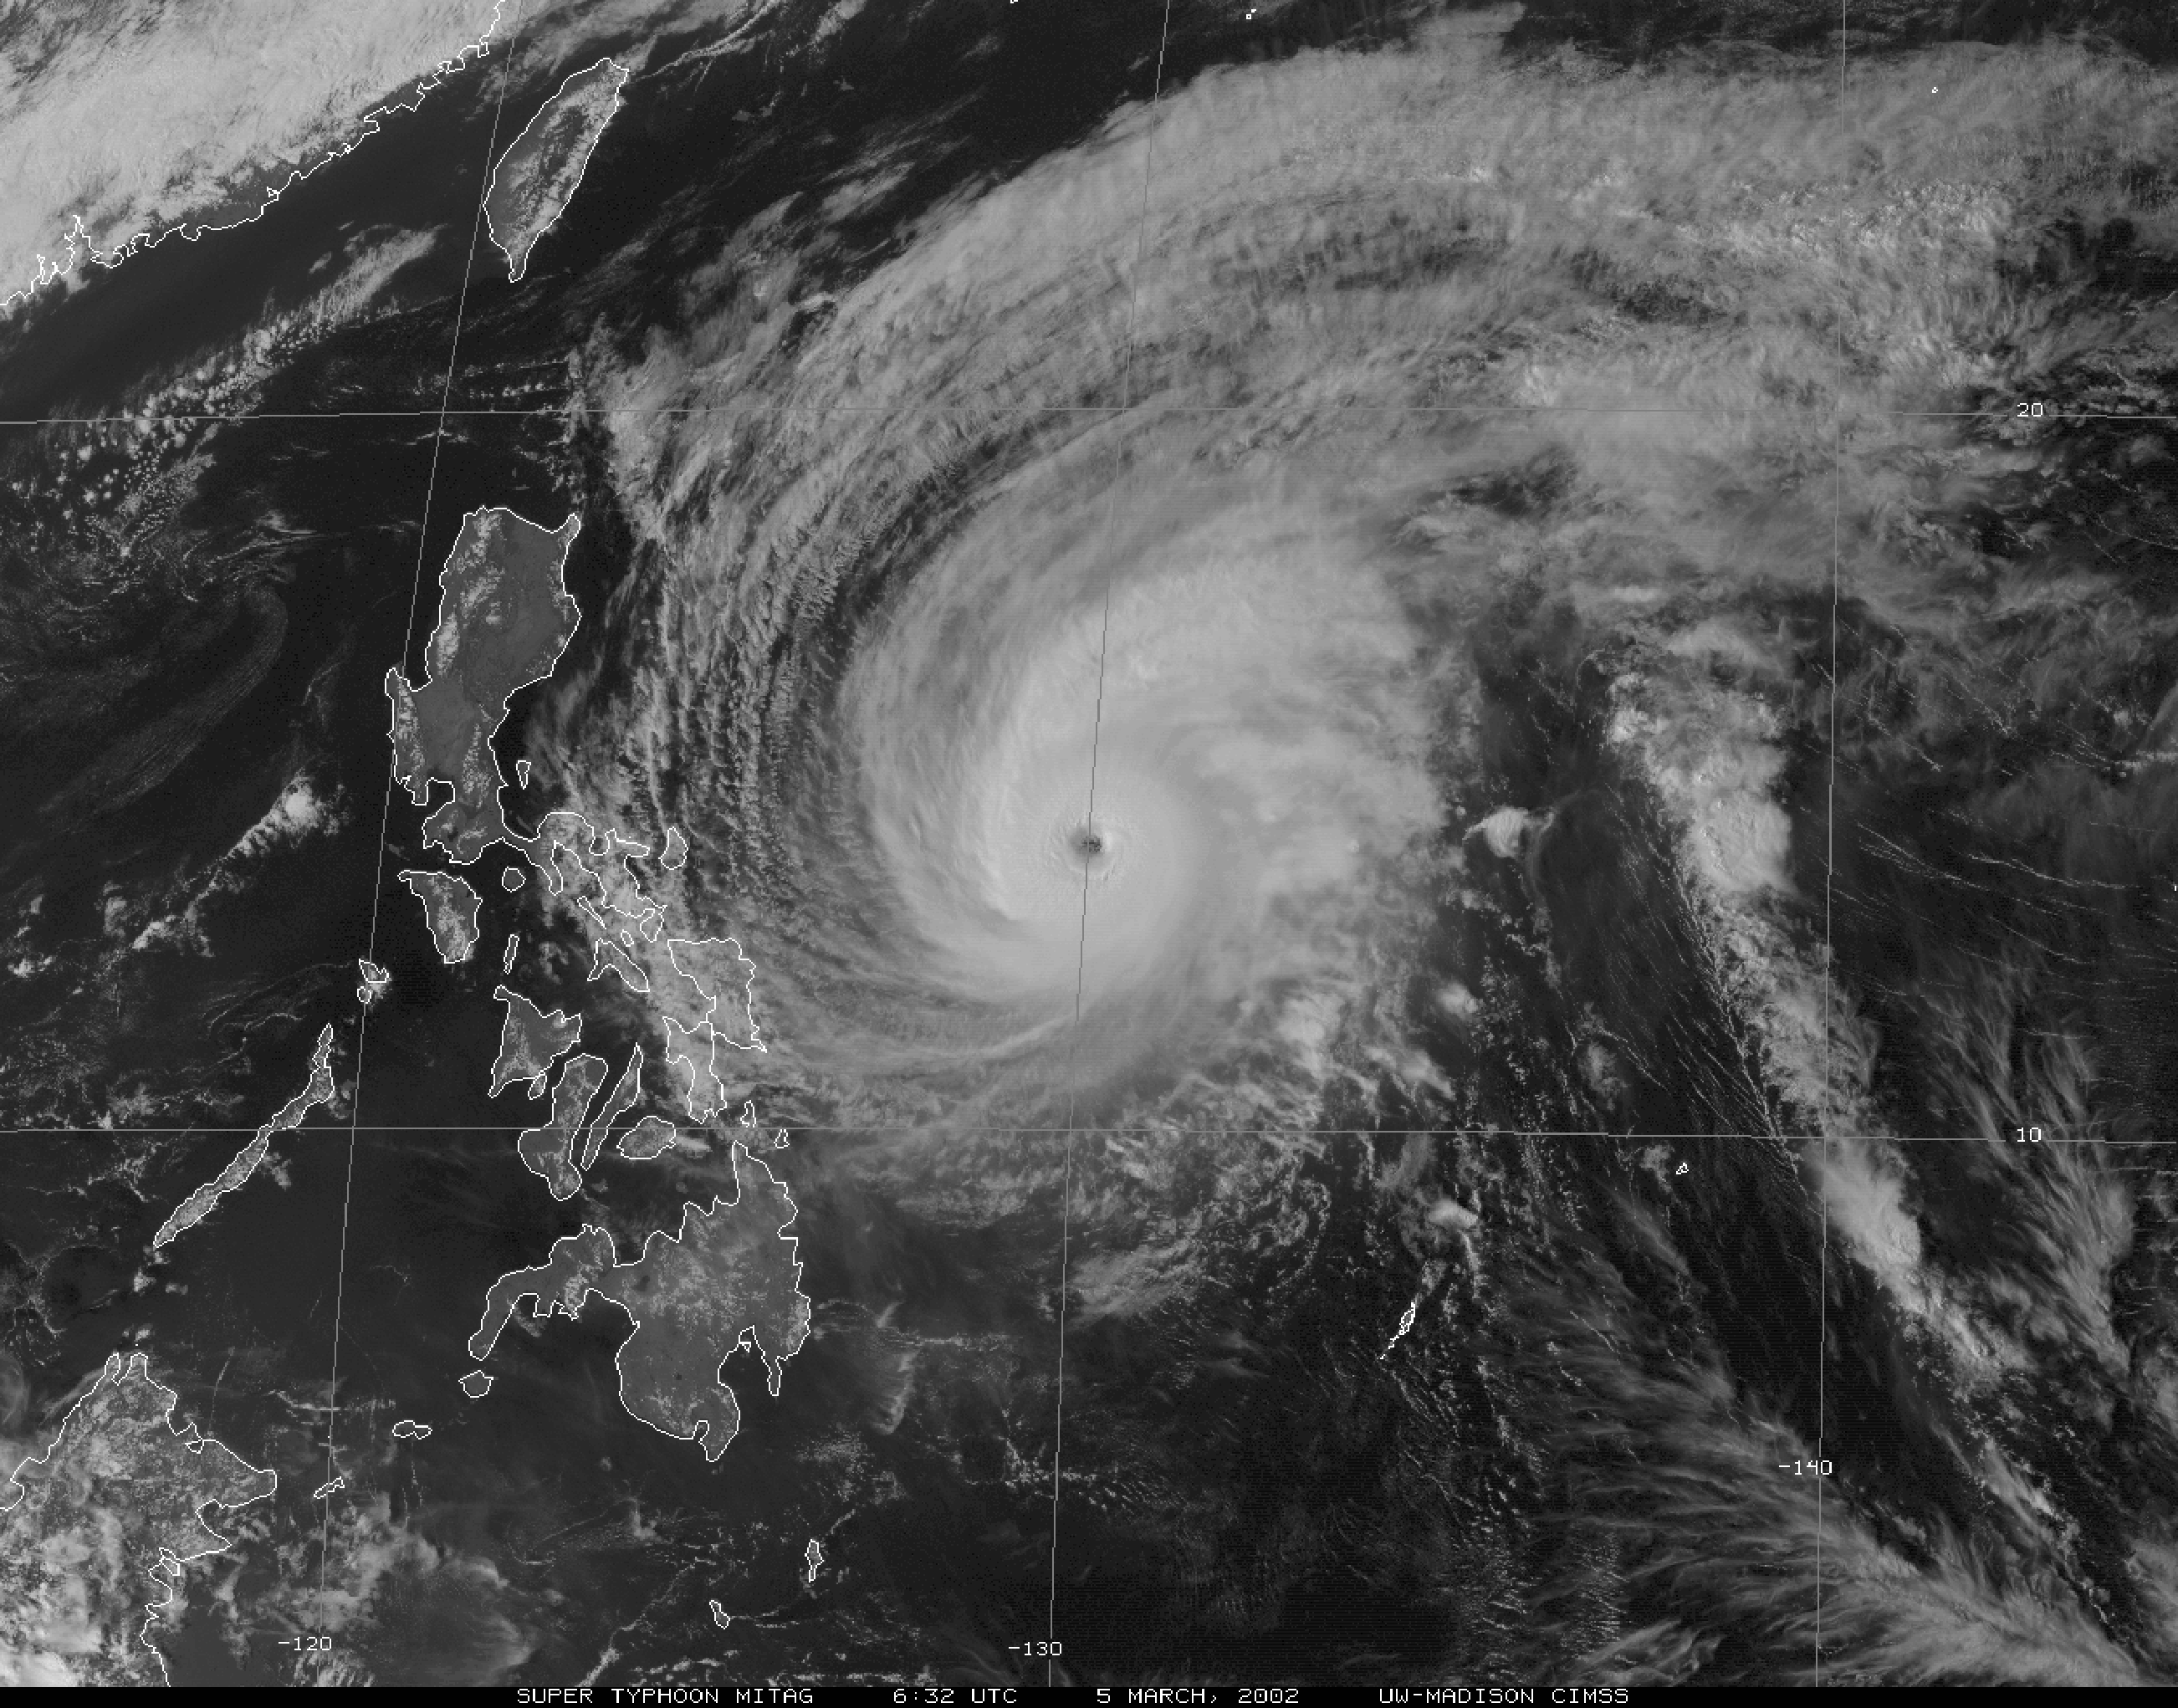
\includegraphics[width=3.5in]{Section2.pdf}}\\
\bigskip
\bigskip
}

\author{\Large{simon.clarke@sci.monash.edu.au}}
\date{\Large{February 2009}}

\maketitle

\newpage 
\subsection*{Bibliography}

\begin{description}
\item[]Acheson, D.J., 1990. Elementary Fluid Dynamics, Oxford University Press.

\item[]Batchelor, G.K., 1967. Introduction to Fluid Dynamics. Cambridge University 
Press.

\item[]Lighthill, J., 1986. An Informal Introduction to Theoretical Fluid 
Mechanics. Oxford University Press.
\end{description}

\subsection*{Acknowledgements}

These notes draw heavily on the lectures given by Professor Bruce Morton and
Professor Michael Reeder at Monash University and Professor Roger Smith
at the University of Munich.

\smallskip
\noindent
The picture overleaf is a Geostationary Meteorological Satellite (GMS) image 
of super typhoon Mitag, 5 March 2002. The image comes from the University of 
Madison, Wisconsin. 



\thispagestyle{empty}
\cleardoublepage

\tableofcontents
\cleardoublepage
% \newpage

\pagenumbering{arabic}

\chapter{Fluid Flow and Conservation of Mass}

\section{Description of fluid flow} The description of a fluid flow requires a
specification or determination of the \textbf{velocity field}, i.e. a
specification of the fluid velocity at every point in the region. In general,
this will define a \textbf{vector field} of position and time, ${\bf u}={\bf
u}({\bf x},t)$.

\textbf{Steady flow} occurs when \textbf{u} is independent of time (i.e.,
${\partial {\bf u}}/{\partial t}=0)$. Otherwise the flow is \textbf{unsteady}.

\begin{figure}[htbp]
\centerline{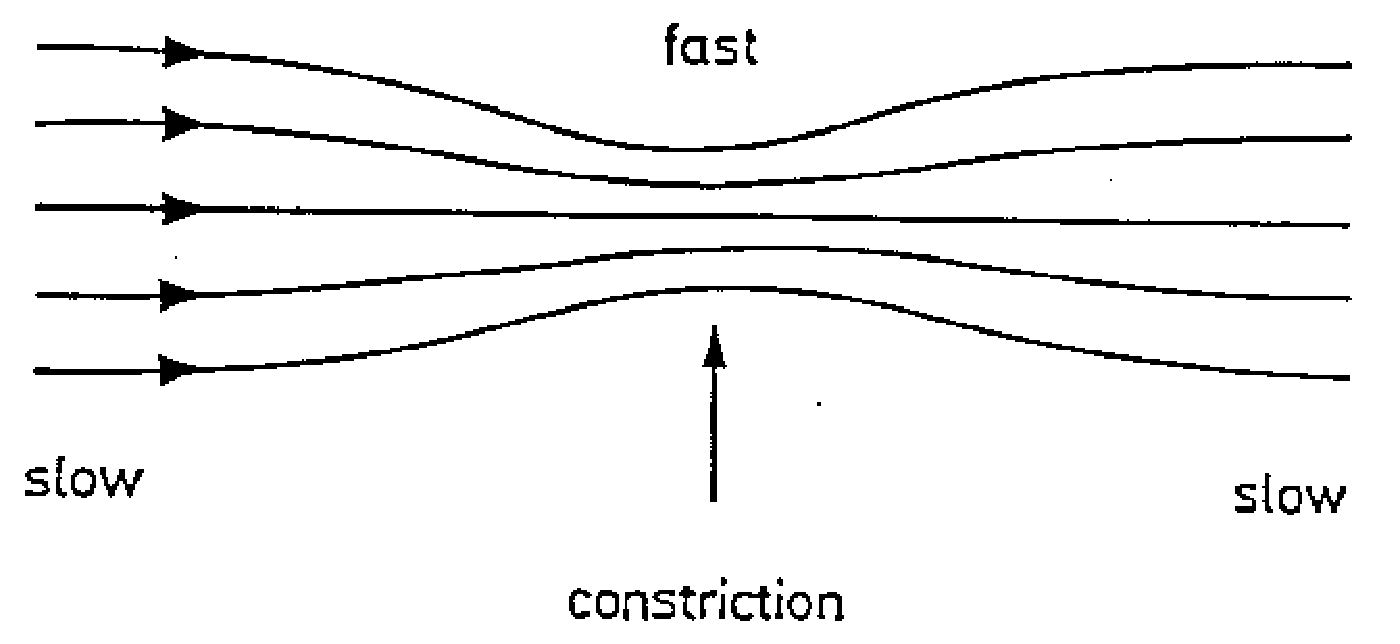
\includegraphics[width=3.5in]{Section3.pdf}}
\label{fig3}
\end{figure}

\textbf{Streamlines} are lines which at a given instant are everywhere in the
direction of the velocity (analogous to electric or magnetic field lines). In
steady flow the streamlines are independent of time, but the velocity can vary
in magnitude along a streamline (as in flow through a constriction in a pipe).

\textbf{Particle paths} are lines traced out by ``marked" particles as time
evolves. In steady flow particle paths are identical to streamlines; in
unsteady flow they are different, and sometimes very different. Particle paths
are visualized in the laboratory using small floating particles of the same
density as the fluid. Sometimes they are referred to as \textbf{trajectories}.

\textbf{Filament lines} or \textbf{streaklines} are traced out over time by
all particles passing through a given point; they may be visualized, for
example, using a hypodermic needle and releasing a slow stream of dye. In
steady flow these are streamlines; in unsteady flow they are neither
streamlines nor particle paths.

It should be emphasized that streamlines represent the velocity field at a
specific instant of time, whereas particle paths and streaklines provide a
representation of the velocity field over a finite period of time. In the
laboratory one can obtain a record of streamlines photographically by seeding
the fluid with small neutrally buoyant particles that move with the flow and
taking a short exposure (e.g. 0.1 sec), long enough for each particle to trace
out a short segment of line; the eye readily links these segments into
continuous streamlines. Particle paths and streaklines are obtained from a
time exposure long enough for the particle or dye trace to traverse the region
of observation.

\section{Equations for streamlines}
\begin{wrapfigure}{r}{3in}
\centerline{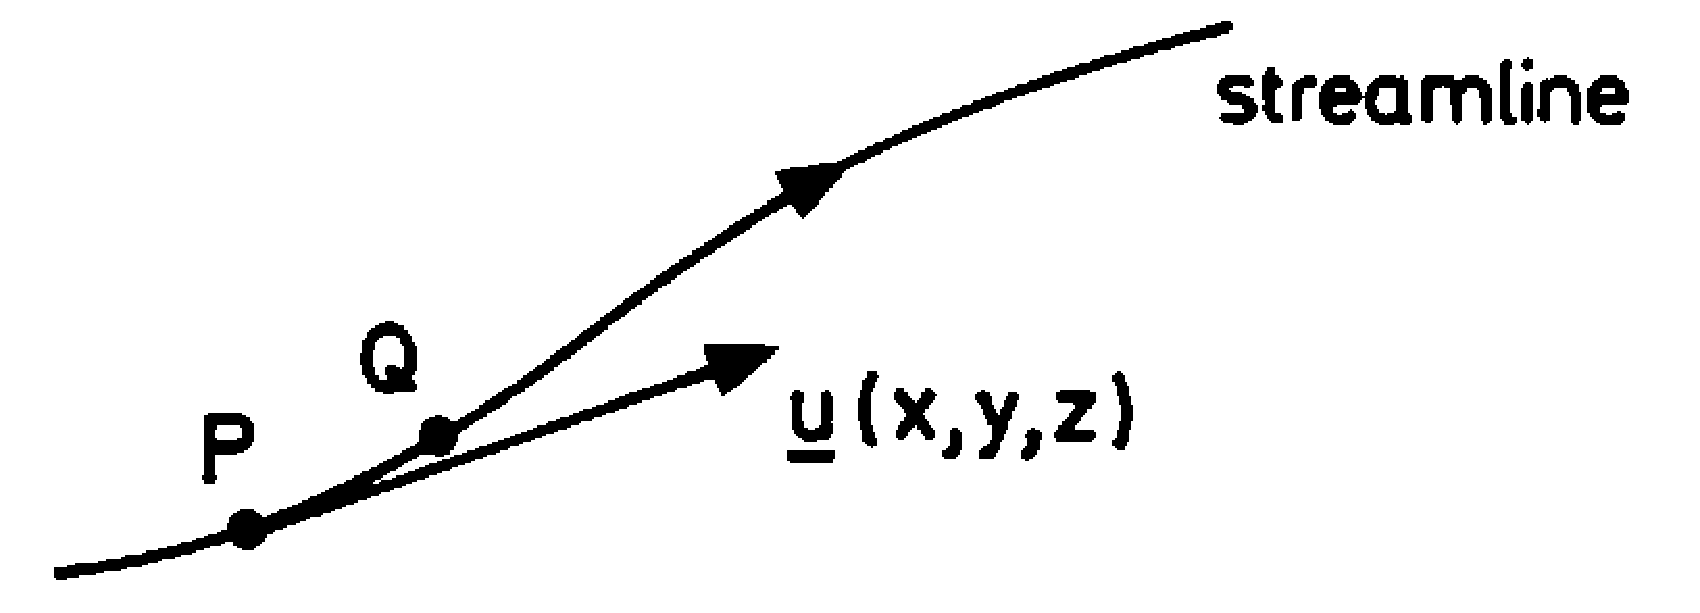
\includegraphics[width=3in]{Section4.pdf}}
\label{fig4}
\end{wrapfigure}

The streamline through the point $P$, say $(x,y,z)$, has the direction of
${\bf u} = (u,v,w)$. Let $Q$ be the neighbouring point $(x + \delta x, y +
\delta y, z + \delta z)$ on the streamline. Then $\delta x \approx u \delta t
, \delta y \approx v \delta t , \delta z \approx w \delta t$ and as $\delta t
\to 0$, we obtain the differential relationship

\begin{equation}
\label{eq11}
\frac{dx}{u}=\frac{dy}{v}=\frac{dz}{w},
\end{equation}
between the displacement $d{\bf x}$ along a streamline and the velocity
components. Equation (\ref{eq11}) gives two differential equations (why?).
Alternatively, we can represent the streamline parametrically (with time as
parameter) as
\begin{equation}
\label{eq2}
\int {\frac{dx}{u}} =\int {dt},\quad \int {\frac{dy}{v}} =\int {dt},\quad  \int {\frac{dz}{w}} =\int {dt} .
\end{equation}

\begin{exmp}
Find the streamlines for the velocity field $u=(-\Omega y, \Omega x,0)$, where $\Omega $ is a constant.

%\textbf{Solution} Equation (\ref{eq1}) gives
%\[
%-\frac{dx}{\Omega y}=\frac{dy}{\Omega x}=\frac{dz}{0}.
%\]
%The first pair of ratios give $\int {\Omega (xdx+ydy)=0} $ or x$^{2}$ + y$^{2}$ = F(z) ,
%where F is an arbitrary function of z. The second pair give $\int {dz} $ = 0 or z = constant.

%Hence the streamlines are circles $x^{2} + y^{2} = c^{2}$ in planes z = constant (we have replaced F(z), a constant when z is constant, by $c^{2}$).

%Note that the velocity at P with position vector \textbf{x} can be expressed as $u=\Omega k\times x$ and corresponds with \textbf{solid body rotation} about the\textbf{ k} axis with angular velocity \textbf{$\Omega$}. (See Exercise 1.4.)
\end{exmp}

Trajectories can be calculated from the definition of the velocity field,
\[
\frac{dx}{dt}=u,
\quad
\frac{dy}{dt}=v,
\quad
\frac{dz}{dt}=w,
\]
where $u=u(x,y,z,t)$, $v=v(x,y,z,t)$ and $w=w(x,y,z,t)$. Generally this is
very difficult as one has to know the velocity field for all time.

\section{Distinctive properties of fluids}
Although fluids are molecular in nature, they can be treated as \textit{continuous} \textit{media} for most 
practical purposes, the exception being rarefied gases.

Real fluids generally show some \textbf{compressibility} defined as 
\[
\frac{1}{\rho }\frac{d\rho 
}{dp}=\frac{\hbox{changes in density per unit change in pressure}}{\hbox{density}},
\]
but at normal atmospheric flow speed, the compressibility of air is a 
relatively small effect and for liquids it is generally negligible. Note that 
sound waves owe their existence to compressibility effects as do ``supersonic 
bangs", produced by aircraft flying faster than sound. For many purposes it 
is accurate to assume our fluids are \textbf{incompressible}, i.e. they 
suffer no change in density with pressure. For the present we shall assume 
also that they are \textbf{homogeneous}, i.e., density $\rho $ = constant.

When one solid body slides over another, \textbf{frictional forces} act 
between them to reduce the relative motion. Friction acts also when layers 
of fluid flow over one another. When two solid bodies are in contact (more 
precisely when there is a normal force acting between them) at rest, there 
is a threshold tangential force \textit{below which} relative motion will not occur. It is 
called the \textbf{limiting friction}. An example is a solid body resting on 
a flat surface under the action of gravity (see figure below).

\begin{figure}[htbp]
\centerline{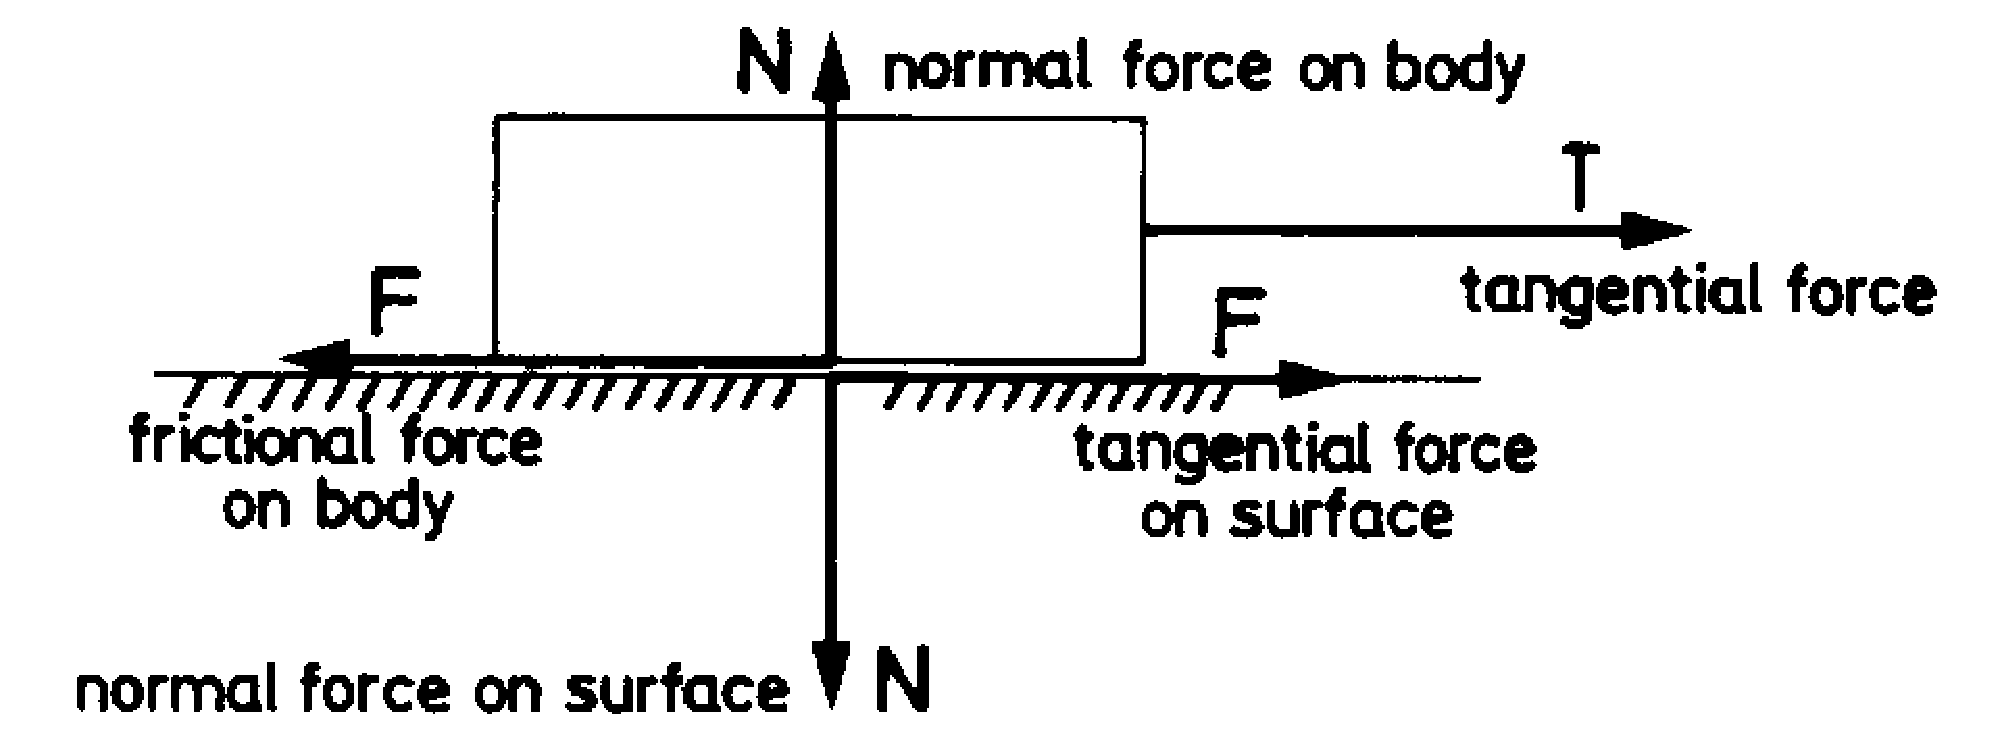
\includegraphics[width=4in]{Section5.pdf}}
\label{fig5}
\end{figure}

As $T$ is increased from zero, $F = T$ until $T = \mu N$, where $\mu $ is the 
so-called coefficient of limiting friction and depends on the degree of roughness 
between the surface. For $T > \quad \mu N$, the body will overcome the 
frictional force and accelerate. A distinguishing characteristic of most 
fluids in their inability to support tangential stresses between layers 
without motion occurring; i.e. there is no analogue of limiting friction. 
Exceptions are certain types of so-called visco-elastic fluids such as 
paint.

Fluid friction is characterized by \textbf{viscosity,} which is a measure of 
the magnitude of tangential frictional forces in flows with velocity 
gradients. \textbf{Viscous forces} are important in many flows, but least 
important in flow past ``streamlined" bodies. We shall be concerned mainly 
with \textbf{inviscid} flows where friction is not important, but it is 
essential to acquire some idea of the sort of flow in which friction may be 
neglected without completely misrepresenting the behaviour. As we shall see, 
neglecting friction is risky!

To begin with we shall be concerned mainly with \textbf{homogeneous, 
incompressible inviscid flows}.

\section{Incompressible flows}
We generalise the idea of a streamline and consider an element of fluid 
bounded by a ``tube of streamlines", known as a \textbf{stream tube.} No 
fluid can cross the walls of the stream tube as they are everywhere in the 
direction of flow.

Hence for incompressible fluids the mass flux ( = mass flow per unit time) 
across section 1 ( = $\rho v_{1}S_{1})$ is equal to that across section 
2 ( = $\rho v_{2}S_{2})$, as there can be no accumulation of fluid 
between these sections. Hence $vS$ = constant and in the limit, for stream 
tubes of small cross-section,
\[
vS = \hbox{\textbf{constant along an elementary stream tube}.}
\]
This result is true for both steady and unsteady flows. The statement is 
obvious for steady flow as the stream tube does not change shape -- think 
about a the analogy with a pipe.

\begin{figure}[htbp]
\centerline{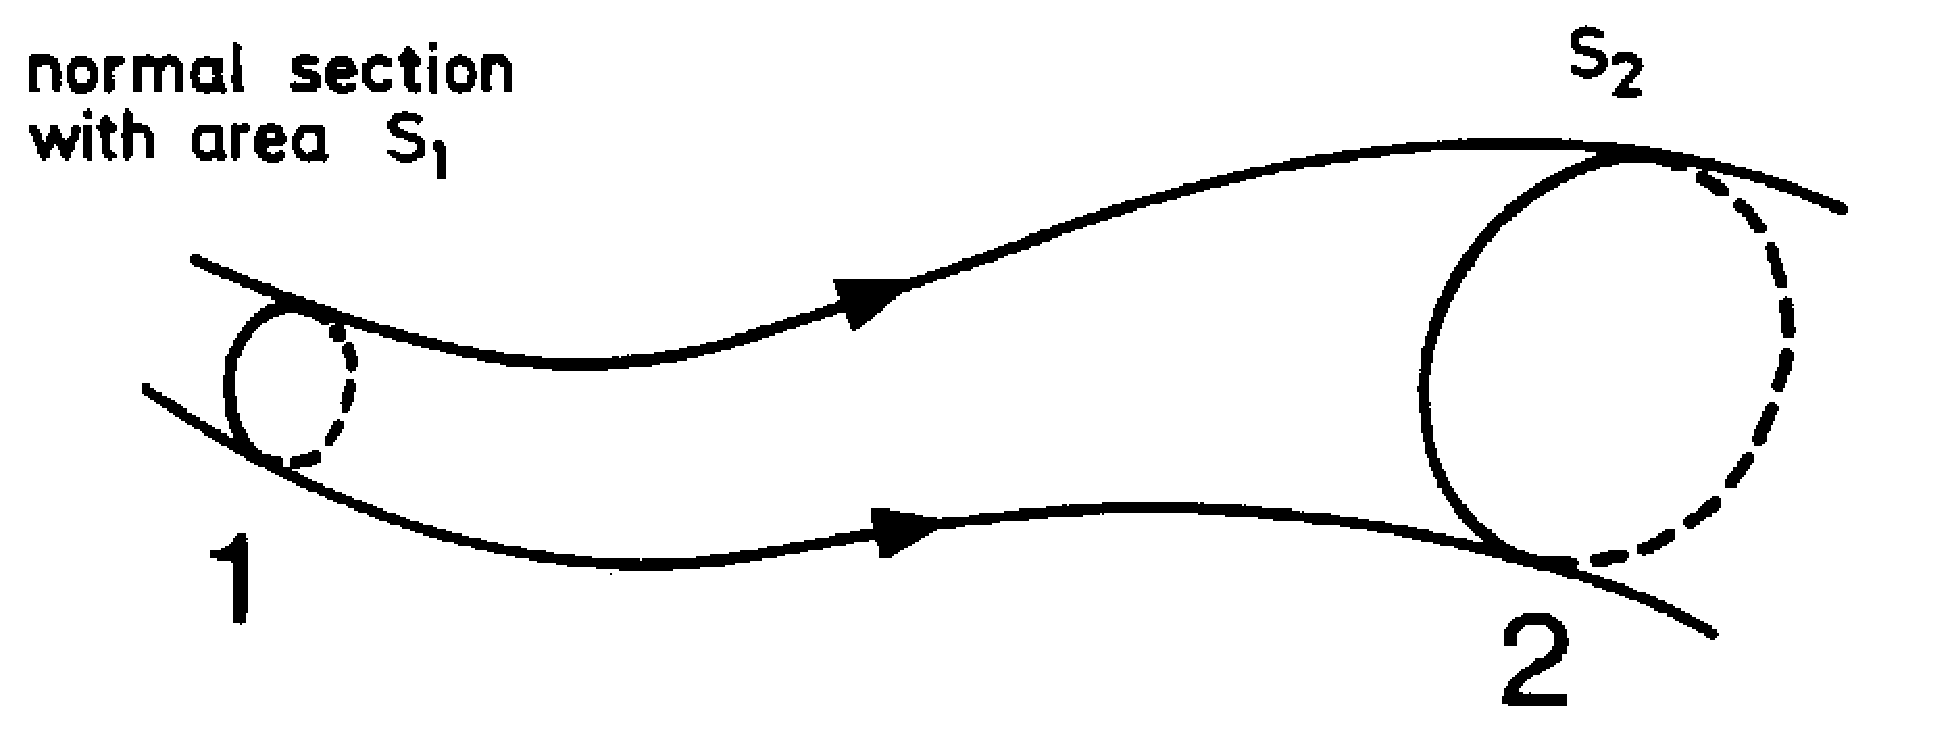
\includegraphics[width=4in]{Section6.pdf}}
\label{fig6}
\end{figure}

It follows that, where streamlines contract the velocity increases, where 
they expand it decreases. Clearly, the streamline pattern contains a great 
deal of information about the velocity distribution.

All vector fields with the property that
\[
\hbox{(vector magnitude)} \times \hbox{(area of tube)}
\]
remains constant along a tube are called \textbf{solenoidal}. The velocity 
field for an incompressible fluid is solenoidal.

\section{Conservation of mass: the continuity equation}

\begin{wrapfigure}{r}{2in}
\centerline{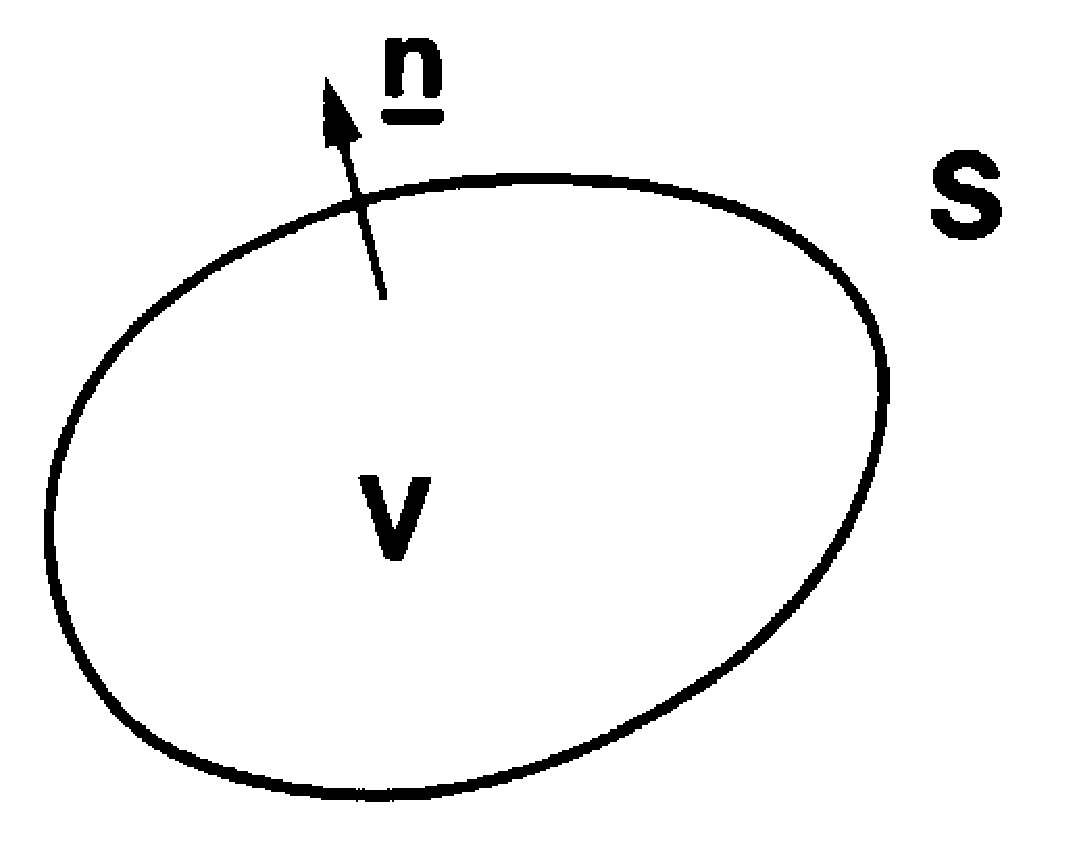
\includegraphics[width=2in]{Section7.pdf}}
\label{fig7}
\end{wrapfigure}


Apply the divergence theorem
\[
\int_V {\nabla . {\bf u} } dV=\int_S {\bf u} . {\bf n}dS
\]
to an arbitrarily chosen volume $V$ with \textbf{closed} surface $S$. 
The mass flux across the elemental area $dS$ is $\rho {\bf u}. 
{\bf n}dS$.

If the fluid is incompressible and there are no mass sources or sinks within 
$S$, then there can be neither continuing accumulation of fluid within $V$ nor 
continuing loss. It follows that the net flux of fluid across the surface $S$ 
must be zero, i.e.,
\[
\int_S  {\bf u} . {\bf n}dS=0,
\]
whereupon. $\int_V {\nabla . {\bf u} } dV=0$. This holds for an 
arbitrary volume $V$, and therefore $\nabla . {\bf u}=0$ throughout an 
incompressible flow without mass sources or sinks. This is the continuity 
equation for a \textbf{homogeneous, incompressible} fluid. It corresponds 
with mass conservation.

\subsection*{Exercises}
\begin{enumerate}
\item Find streamlines for the velocity field ${{\bf u}}=(\alpha x,-\alpha
y,0)$, where $\alpha $ is constant, and sketch them for the case $\alpha > 0$.
\item Consider the unsteady flow ${{\bf u}}=(u_0 ,kt,0)$, where $u_{0}$ and
$k$ are positive constants. Show that the streamlines are straight lines, and
sketch them at two different times. Also show that the fluid follows a
parabolic path as time proceeds. 
\item Consider the velocity field defined by
${{\bf u}}=(e^{-t}z,0,0)$. Calculate the parcel trajectories. 
\item Show that
the expression $u=\Omega {\bf k}\times {\bf x}$ describes solid body rotation
about the\textbf{ k} axis with angular velocity $\Omega $. 
\item A stream is
broad and shallow with width 8 m, mean depth 0.5 m and mean speed 1~m
s$^{-1}$. What is its volume flux (rate of flow per second) in m$^{3}$
s$^{-1}$? It enters a pool of mean depth 3 m and width 6 m: what then is its
mean speed? It continues over a waterfall in a single column with mean speed
10 ms$^{-1}$ at its base: what is the mean diameter of this column at the base
of the waterfall? Will the diameter of the water column at the top of the
waterfall be greater, equal to, or less at its base? Why? 
\end{enumerate}

\cleardoublepage

\chapter{Equation of Motion}
\section{Newton's Second Law}
The equation of motion is an expression of Newton's second law:
\[
\hbox{\textbf{mass}}\times \hbox{\textbf{acceleration = force.}}
\]
However, in contrast to the case of rigid-body dynamics, we need to apply an 
additional constraint, a continuity equation, or mass-conservation equation. 
Because of this constraint, it is not possible, in general, to specify the 
\textit{force}, or more precisely \textit{force field} independently, as in rigid body problems. 

To apply Newton's second law we must focus our attention on a particular 
element of fluid, say the small rectangular element, which at time $t$ has 
vertex at $P [=(x,y,z)$] and edges of length $\delta x$, $\delta y$, $\delta 
z$. The mass of this element is $\rho\ \delta x \delta y\delta z$, 
where $\rho $ is the fluid \textbf{density} (or mass per unit volume), which 
we shall assume constant.

\begin{figure}[htbp]
\centerline{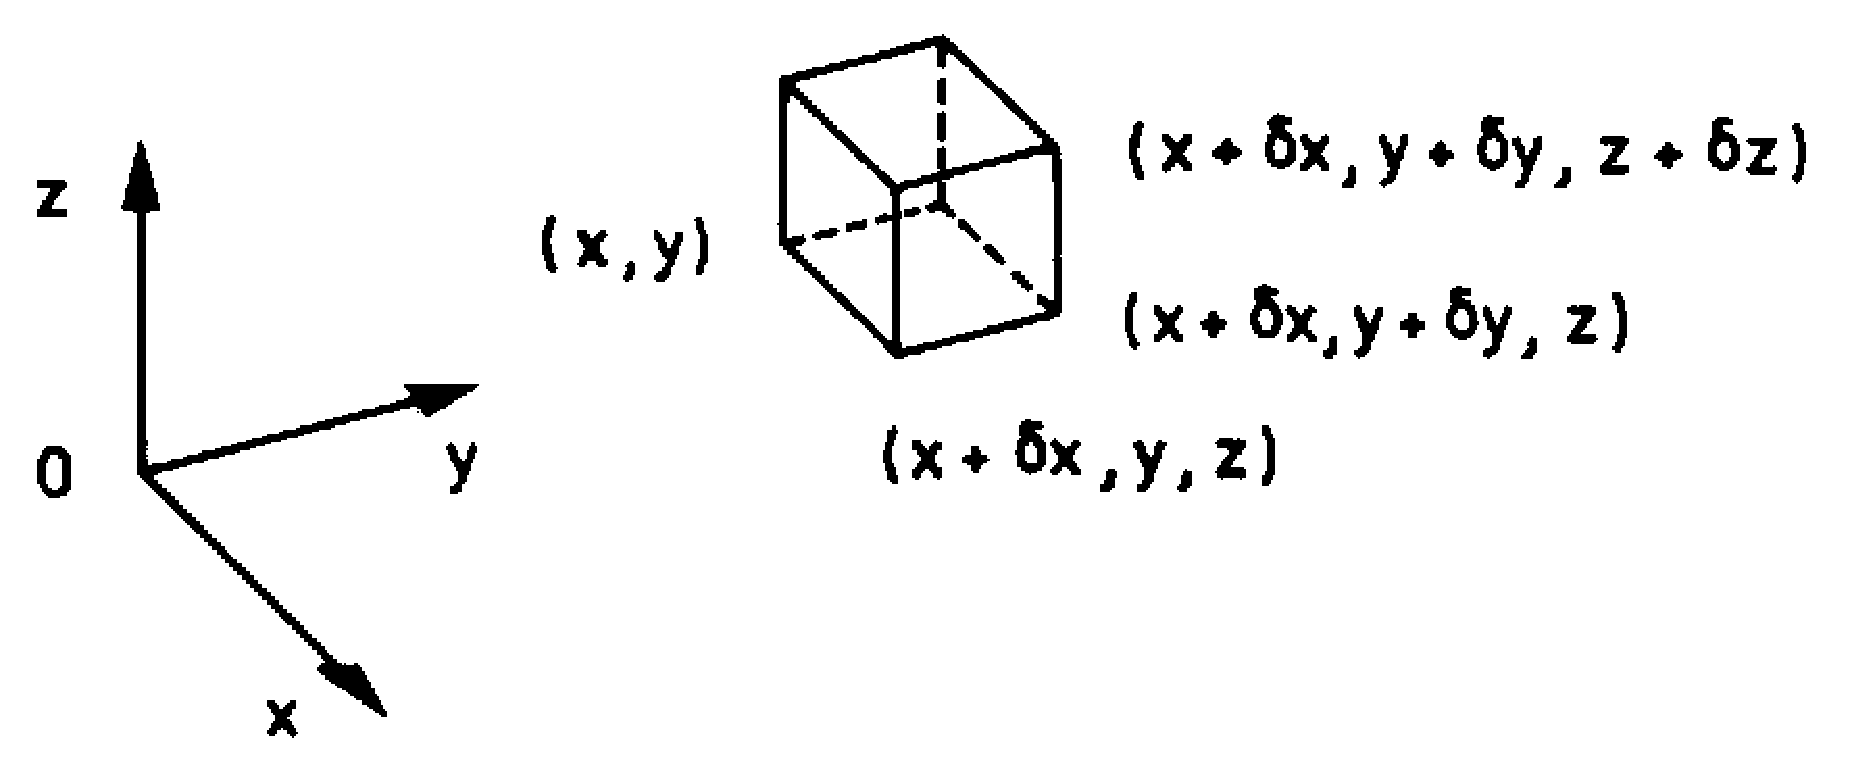
\includegraphics[width=4.5in]{Section21.pdf}}
\label{fig1}
\end{figure}

The velocity in the fluid, ${\bf u} = {\bf u}(x,y,z)$ is a function both of 
position $(x,y,z)$ and time $t$, and from this we must derive a formula for the 
acceleration of the element of fluid which is changing its position with 
time. Consider, for example, steady flow through a constriction in a pipe 
(see the first diagram in Chapter 1). Elements of fluid must accelerate into 
the constriction as the streamlines close in and decelerate beyond as they 
open out again. Thus, in general, the acceleration of an element (i.e., the 
rate of change of \textbf{u} with time for that element) includes a rate of 
change at a fixed position $\partial {\bf u}/\partial t$ plus a change 
associated with its change of position with time. We derive an expression 
for the latter below.

The forces acting on the elements $\delta x\ \delta y\ \delta z$ comprise:
\begin{description}
\item[(i)] \textbf{body forces}, which are forces per unit mass acting throughout 
the fluid because of external causes, such as the gravitational 
\textbf{weight}, and
\item[(ii)] \textbf{contact forces} acting across the surface of the element from 
adjacent elements.
\end{description}
These are discussed further below.

\section{Rate-of-change moving with the fluid}
We consider first the rate of change of a scalar property, for example the 
temperature of a fluid, following a fluid element. The temperature of a 
fluid, $T = T(x,y,z,t)$, comprises a scalar field in which $T$ will vary, in 
general, both with the position and with time (as in the water in a kettle 
which is on the boil). Suppose that an element of fluid moves from 
$P[=(x,y,z)]$ at time $t$ to $Q[=(x+\delta 
x,y+\delta y,z+\delta z)]$at time $ t + \delta t$. 
Note that if we stay at a particular point $(x_{0},y_{0},z_{0})$, then 
$T(x_{0},y_{0},z_{0},t)$ is effectively a function of $t$ only, but that 
if we move with the fluid, $T(x,y,z)$ is a function both of position $(x,y,z)$ 
and time $t$. It follows that the total change in $T$ between $P$ and $Q$ in time 
$\delta t$ is
\[
\delta T=T_Q -T_P =T(x+\delta 
x,y+\delta y,z+\delta z,t+\delta 
t)-T(x,y,z,t)\quad ,
\]
and hence the total rate of change of $T$ moving with the fluid is
\[
\mathop {\lim }\limits_{\delta t\to 0} \frac{\delta T}{\delta 
t}=\mathop {\lim }\limits_{\delta t\to 0} 
\frac{T(x+\delta x,y+\delta 
y,z+\delta z,t+\delta 
t)-T(x,y,z,t)}{\delta t}.
\]
For small increments $\delta x$, $\delta y$, $\delta z$, $\delta t$ we may 
use a Taylor expansion
\begin{align*}
&T(x+\delta x,y+\delta y,z+\delta 
z,t+\delta t) \\
& =T(x,y,z,t)+\left[ 
{\frac{\partial T}{\partial x}} \right]_P \delta x+
\left[ {\frac{\partial T}{\partial y}} \right]_P \delta y+\left[ 
{\frac{\partial T}{\partial z}} \right]_P \delta z+\left[ 
{\frac{\partial T}{\partial t}} \right]_P \delta t \\
& \quad + 
\hbox{higher order terms in }\delta 
x,\delta y,\delta z,\delta t. 
\end{align*}
Hence the rate of change moving with the fluid element
\begin{align*}
\mathop {\lim }\limits_{\delta t\to 0} \frac{\delta T}{\delta 
t}
&=\mathop {\lim }\limits_{\delta t\to 0} \left[ {\frac{\partial 
T}{\partial t}\delta t+\frac{\partial T}{\partial x}\delta 
x+\frac{\partial T}{\partial y}\delta y+\frac{\partial 
T}{\partial z}\delta z} \right]/\delta t
\\
&
=\frac{\partial T}{\partial t}+u\frac{\partial T}{\partial 
x}+v\frac{\partial T}{\partial y}+w\frac{\partial 
T}{\partial z}
\end{align*}
since higher order terms $\to0$ and $u = dx/dt$, $v = dy/dt$, $w = dz/dt$, where 
${\bf x} = {\bf x}(t)$ is the coordinate vector of the 
moving fluid element. To emphasize that we mean the \textbf{total rate of 
change moving with the fluid} we write
\begin{equation}
\label{eq1}
\frac{DT}{Dt}=\frac{\partial T}{\partial t}+u\frac{\partial T}{\partial 
x}+v\frac{\partial T}{\partial y}+w\frac{\partial T}{\partial z}\quad .
\end{equation}
Here, $\partial T/\partial t$ is the \textbf{local rate of change} with 
time at a fixed position $(x,y,z)$, while 
\[
u\frac{\partial T}{\partial x}+v\frac{\partial T}{\partial 
y}+w\frac{\partial T}{\partial z}={\bf u}. \nabla T
\]
is the \textbf{advective rate of change} associated with the movement of the 
fluid element.

\begin{exmp}
Show that 
\[ \frac{D{{\bf F}}}{Dt}=\frac{\partial {{\bf F}}}{\partial 
t}+\left( {{{\bf u}}. \nabla } \right){{\bf F}}\]
represents the 
total rate-of-change of any vector field ${\bf F}$ moving with the fluid 
velocity (velocity field ${\bf u}$), and in particular that the 
acceleration (or total change in ${\bf u}$ moving with the fluid) is 
\[ \frac{D{{\bf u}}}{Dt}=\frac{\partial {{\bf u}}}{\partial t}+\left( 
{{{\bf u}}. \nabla } \right){{\bf u}}. \]

%\textbf{Solution} The previous result for the rate-of-change of a scalar 
%field can be applied to each of the component of \textbf{F}, or to each of 
%the velocity components (u,v,w) and these results follow at once.
\end{exmp}

\begin{exmp}
Show that \[\frac{D{{\bf x}}}{Dt}={{\bf u}}\]

%\textbf{Solution}
%\[
%\begin{array}{l}
% \frac{D{{\bf x}}}{Dt}=\frac{\partial {{\bf x}}}{\partial t}+\left( 
%{{{\bf u}}. \nabla } \right){{\bf x}} \\ 
% =0+\left( {u\frac{\partial }{\partial x}+v\frac{\partial }{\partial 
%y}+w\frac{\partial }{\partial z}} \right)\left( {x,y,z} \right) \\ 
% =\left( {u,v,w} \right) \\ 
% \end{array}
%\]
%as x, y, z, t are independent variables.
\end{exmp}

\section{Internal forces in a fluid (see Acheson p. 203)}
An element of fluid experiences \textit{contact} or internal forces across its surface due 
to the action of adjacent elements. These are in many respects similar to 
the normal reaction and tangential friction forces exerted between two rigid 
bodies, except, as noted earlier, friction in fluids acts only when the 
fluid is in non-uniform motion.

\begin{wrapfigure}{r}{2.5in}
\centerline{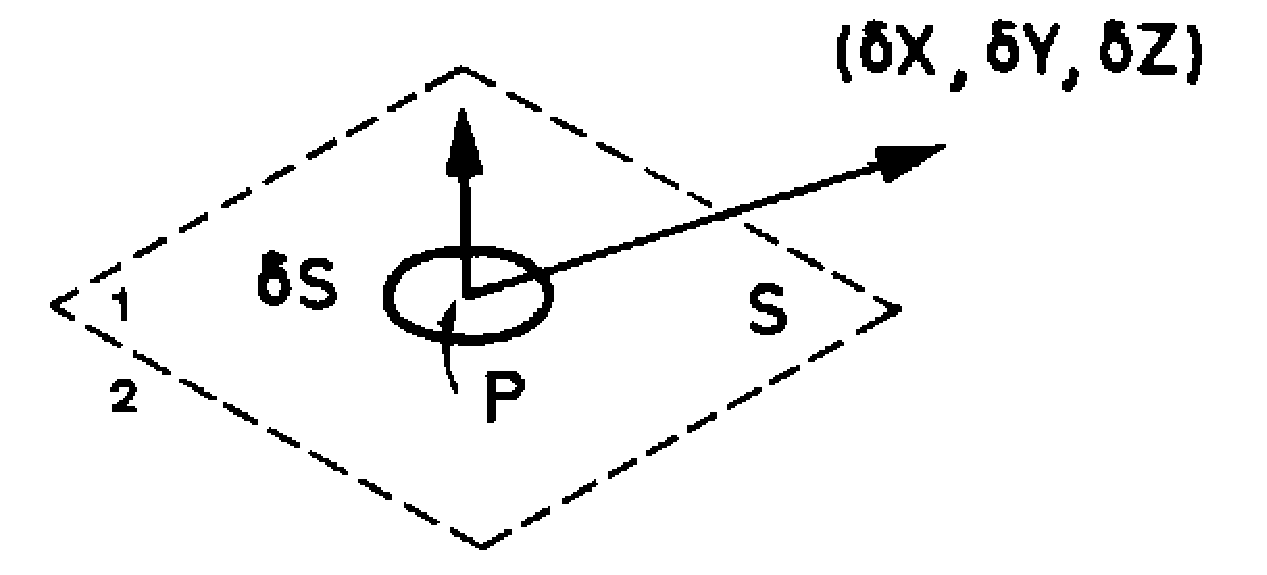
\includegraphics[width=2.5in]{Section22.pdf}}
\label{fig2}
\end{wrapfigure}

Consider a region of fluid divided into two parts by the (imaginary) surface 
$S$, and let $\delta S$ be a small element of $S$ containing the point $P$ and 
with region 1 below and region 2 above $S$. Let $(\delta X, \delta Y, 
\delta Z)$ denote the force exerted \textbf{on} fluid in region 1 
\textbf{by} fluid region 2 across $\delta S$.

This elementary force is the resultant (vector sum) of a set of contact 
forces acting across $\delta S$, in general it will not act through $P$; 
alternatively, resolution of the forces will yield a force ($\delta X$, 
$\delta Y$, $\delta Z$) acting through $P$ together with an elementary couple 
with moment of magnitude on the order of $(\delta S)^{1/2}(\delta 
X^2+\delta Y^2+\delta Z^2)^1/2$, which $\to  0$ as $\delta S \to 0$. 

The main force per unit area exerted by fluid 2 on fluid 1 across $\delta 
S$,
\[
\left[ {\frac{\delta X}{\delta S},\frac{\delta Y}{\delta 
S},\frac{\delta Z}{\delta S}} \right]
\]
is called the \textbf{mean stress}. The limit as $\delta S \to  0$ in such 
a way that it always contains $P$, if it exists, is the \textbf{stress} at $P$ 
across $S$. Stress is a force per unit area. The stress ${\bf F}$ is 
generally inclined to the normal ${\bf n}$ to $S$ at $P$, and varies both in 
magnitude and direction as the orientation ${\bf n}$ of $S$ is varied about 
the fixed point $P$.

The stress  ${\bf F}$ may be resolved into a \textbf{normal reaction} $N$, or 
\textbf{tension}, acting normal to $S$ and \textbf{shearing stress} $T$, 
tangential to $S$, each per unit area.

\begin{figure}[htbp]
\centerline{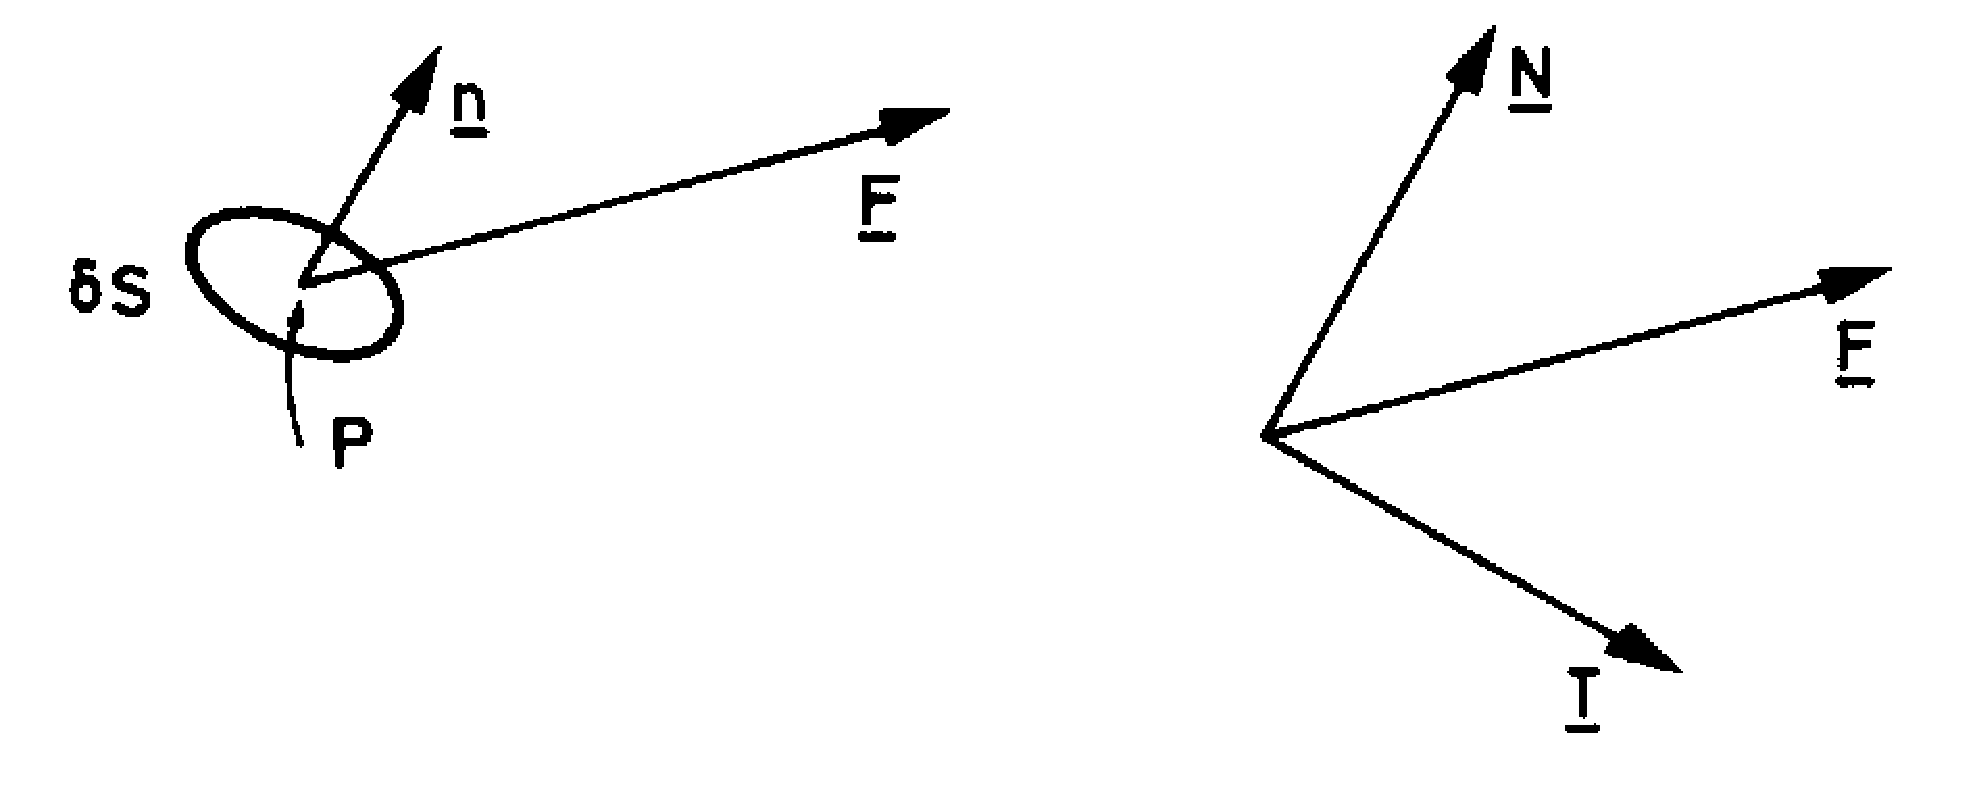
\includegraphics[width=4in]{Section23.pdf}}
\label{fig3}
\end{figure}

The stress and its reaction (exerted by fluid in region 1 on fluid in region 
2) are equal and opposite. [This follows by considering the equilibrium of 
an infinitesimal slice at $P$].

\begin{figure}[htbp]
\centerline{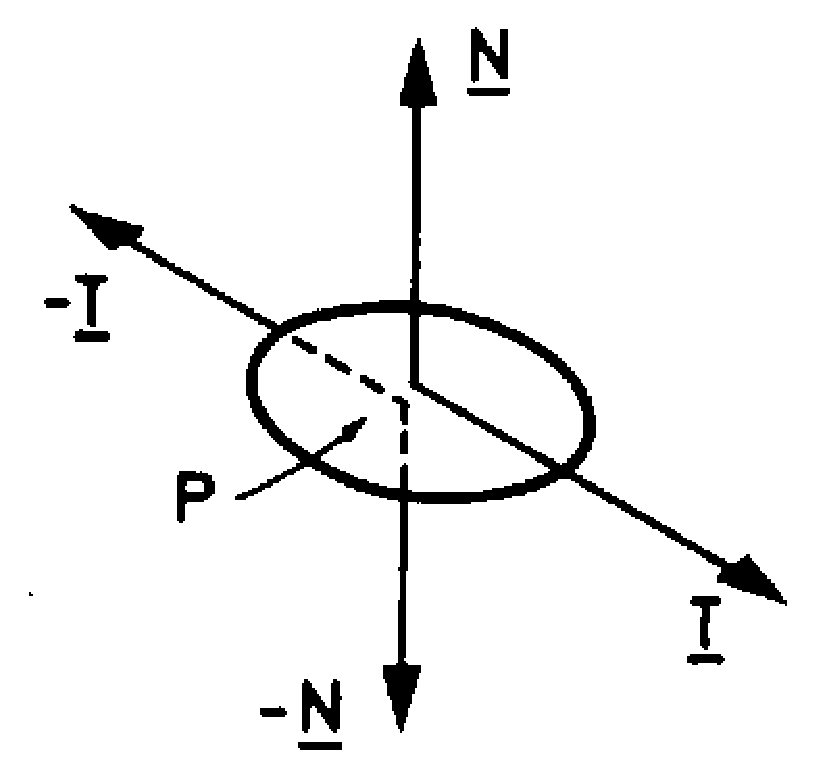
\includegraphics[width=2in]{Section24.pdf}}
\label{fig4}
\end{figure}

\section{Fluid and solids: pressure}
If the stress in a material \textbf{at rest }(or in uniform motion) is 
always normal to the measuring surface for all points $P$ and surfaces $S$, the 
material is termed a \textbf{fluid}; otherwise it is a \textbf{solid}. 
Solids at rest sustain tangential stresses because of their elasticity (for 
example, a drawn bow). By assuming the material to be at rest we eliminate 
the shearing stress due to internal friction. Many real fluids conform 
closely to this definition including air and water (although there are more 
complex fluids possessing both viscosity and elasticity). A fluid can be 
defined also as a material offering no \textbf{initial} resistance to shear 
stress, although it is important to realize that frictional shearing 
stresses appear as soon as motion begins, and even the smallest force will 
initiate motion in a fluid in time. The property of internal friction in a 
fluid is known as \textbf{viscosity}.

Although the term tension is usual in the theory of elasticity, in fluid 
dynamics the term \textbf{pressure} is used to denote the hydrostatic 
stress, reversed in sign. In a fluid at rest the stress acts normally 
outwards from a surface, whereas the pressure thrust acts normally 
\textbf{inwards} from the fluid towards the surface.

Physically, pressure is the transfer of momentum per unit area per unit time 
(the momentum flux) across any surface $\delta S$.

\subsection{Isotropy of pressure}
The pressure at a point $P$ in a continuous fluid is \textbf{isotropic}; i.e., 
it is the same for all directions ${\bf n}$. This is proved by considering 
the equilibrium of a small tetrahedral element of fluid with three faces 
normal to the coordinate axes and one slant face. The proof may be found in 
any text on fluid mechanics.

In an ideal fluid the force exerted on the fluid separated by a small 
imaginary surface ${\bf n}\delta S$ is $p{\bf n}\delta S$. The 
\textbf{pressure thrust} on a surface is the gross force on the surface due 
to pressure acting normally inwards, i.e.$\int_S {-p{{\bf n}}dS} 
$ evaluated over the surface $S$. The pressure is independent  of the 
surface element chosen.

\subsection{Pressure gradient forces in a fluid in macroscopic equilibrium}
Pressure is independent of direction at a point, but may vary from point to 
point in a fluid.

Consider the equilibrium of a thin cylindrical element of fluid $PQ$ of length 
$\delta s$ and cross-section $A$, and with its ends normal to $PQ$. In particular, 
consider the 
forces in the direction $P$ for the fluid at rest. Then pressure acts normally 
inwards on the curved cylindrical surface and has no component in the 
direction of $PQ$. Thus the only contributions are from the plane ends.

\begin{figure}[htbp]
\centerline{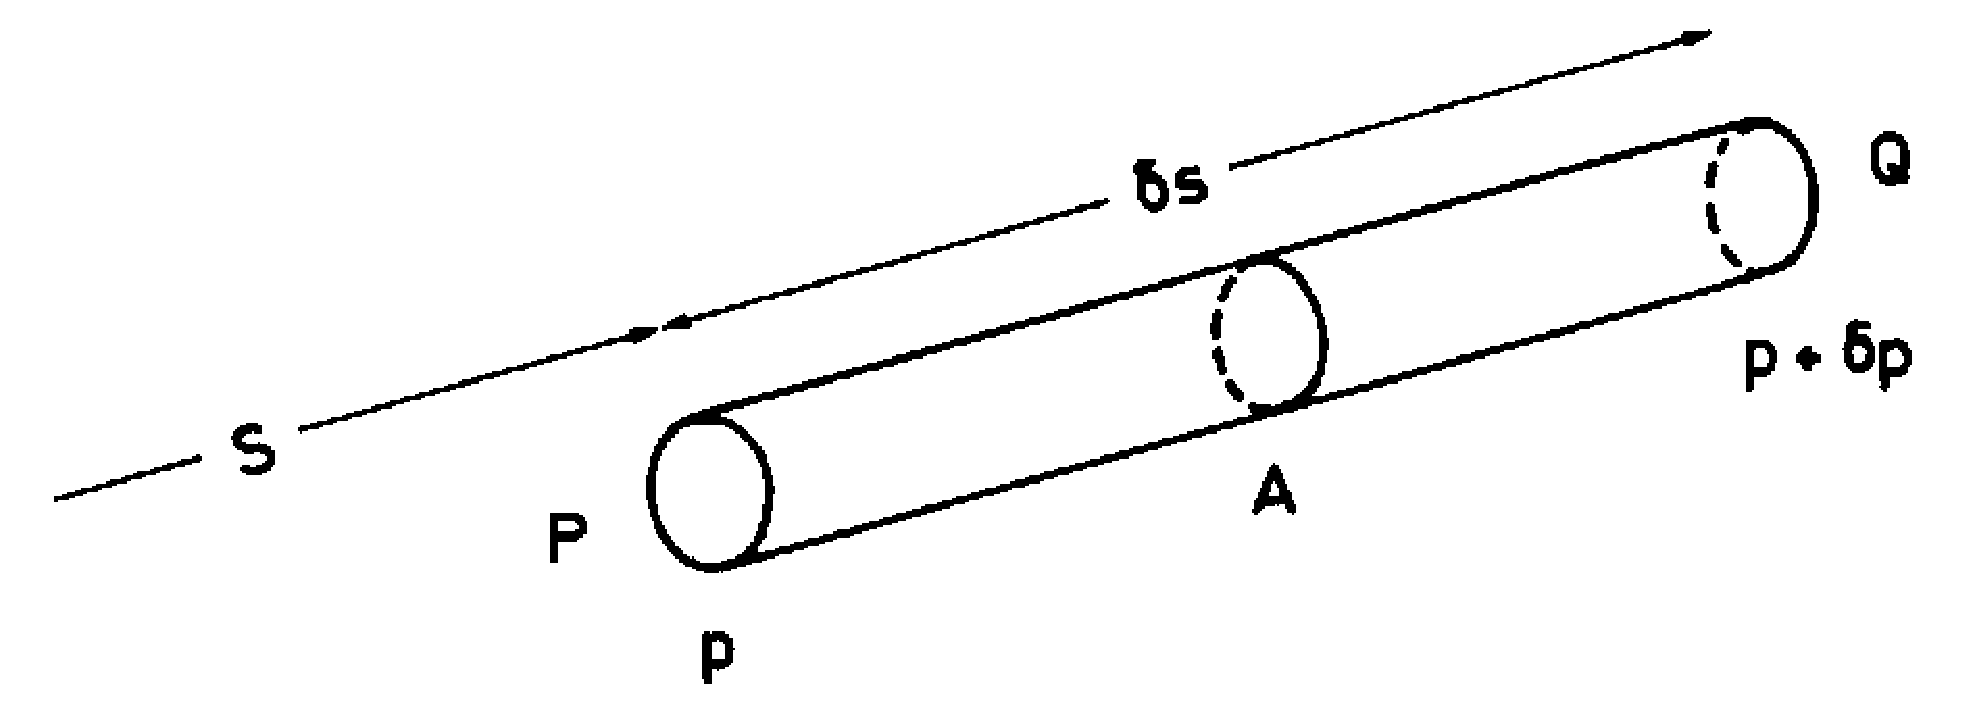
\includegraphics[width=3in]{Section25.pdf}}
\label{fig5}
\end{figure}

The net force in the direction in the direction $s$ (i.e. the direction $PQ$) 
due to the pressure thrusts on the surface of the element is
\[
pA-(p+\delta p)A=-\frac{\partial p}{\partial 
s}A\delta s=-\frac{\partial p}{\partial s}\delta V,
\]
where $\delta V$ is the volume of the cylinder. In the limit $\delta s \to 
 0$ and $A \to  0$, the net pressure thrust $\to -(\partial 
p/\partial s)dV$, or $-\partial p/\partial 
s=-{\bf \hat {s}}. \nabla p$ per unit volume of 
fluid ($-{{\bf \hat {s}}}$ being a unit vector in the direction $PQ$). It 
follows that -$\nabla p$ is the pressure gradient force per unit volume of 
fluid, and $-{{\bf \hat {n}}}. \nabla p$ is the component of 
pressure gradient force per unit volume in a given direction ${{\bf \hat 
{n}}}$.

\begin{wrapfigure}{r}{2.5in}
\centerline{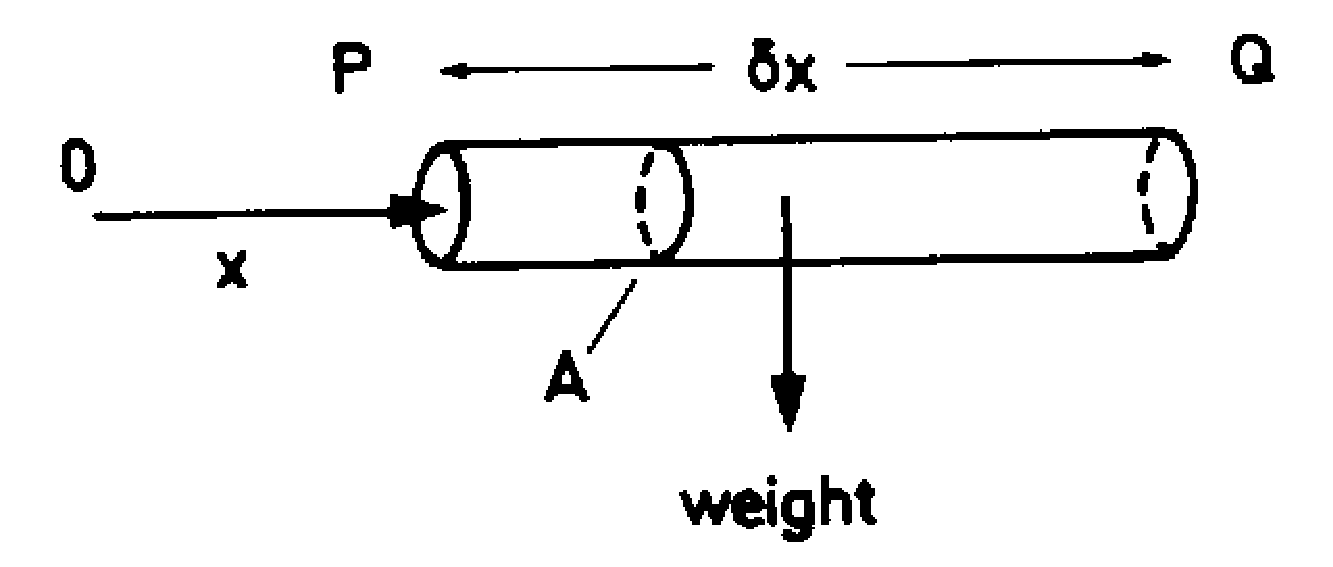
\includegraphics[width=2.5in]{Section26.pdf}}
\label{fig6}
\end{wrapfigure}

The cylindrical element shown right is in equilibrium under the action of 
the pressure over its surface and its weight. The horizontal component of 
pressure gradient force per unit volume is $-{{\bf i}}. 
\nabla p=-\partial p/\partial x=0$.

Thus $p$ is independent of horizontal distance $x$, and is similarly independent 
of horizontal distance $y$. It follows that $p = p(z)$ and surfaces of equal 
pressure (\textbf{isobaric surfaces}) are horizontal in a fluid at rest.

\subsection{Equilibrium of a vertical element}

\begin{wrapfigure}{r}{2.5in}
\centerline{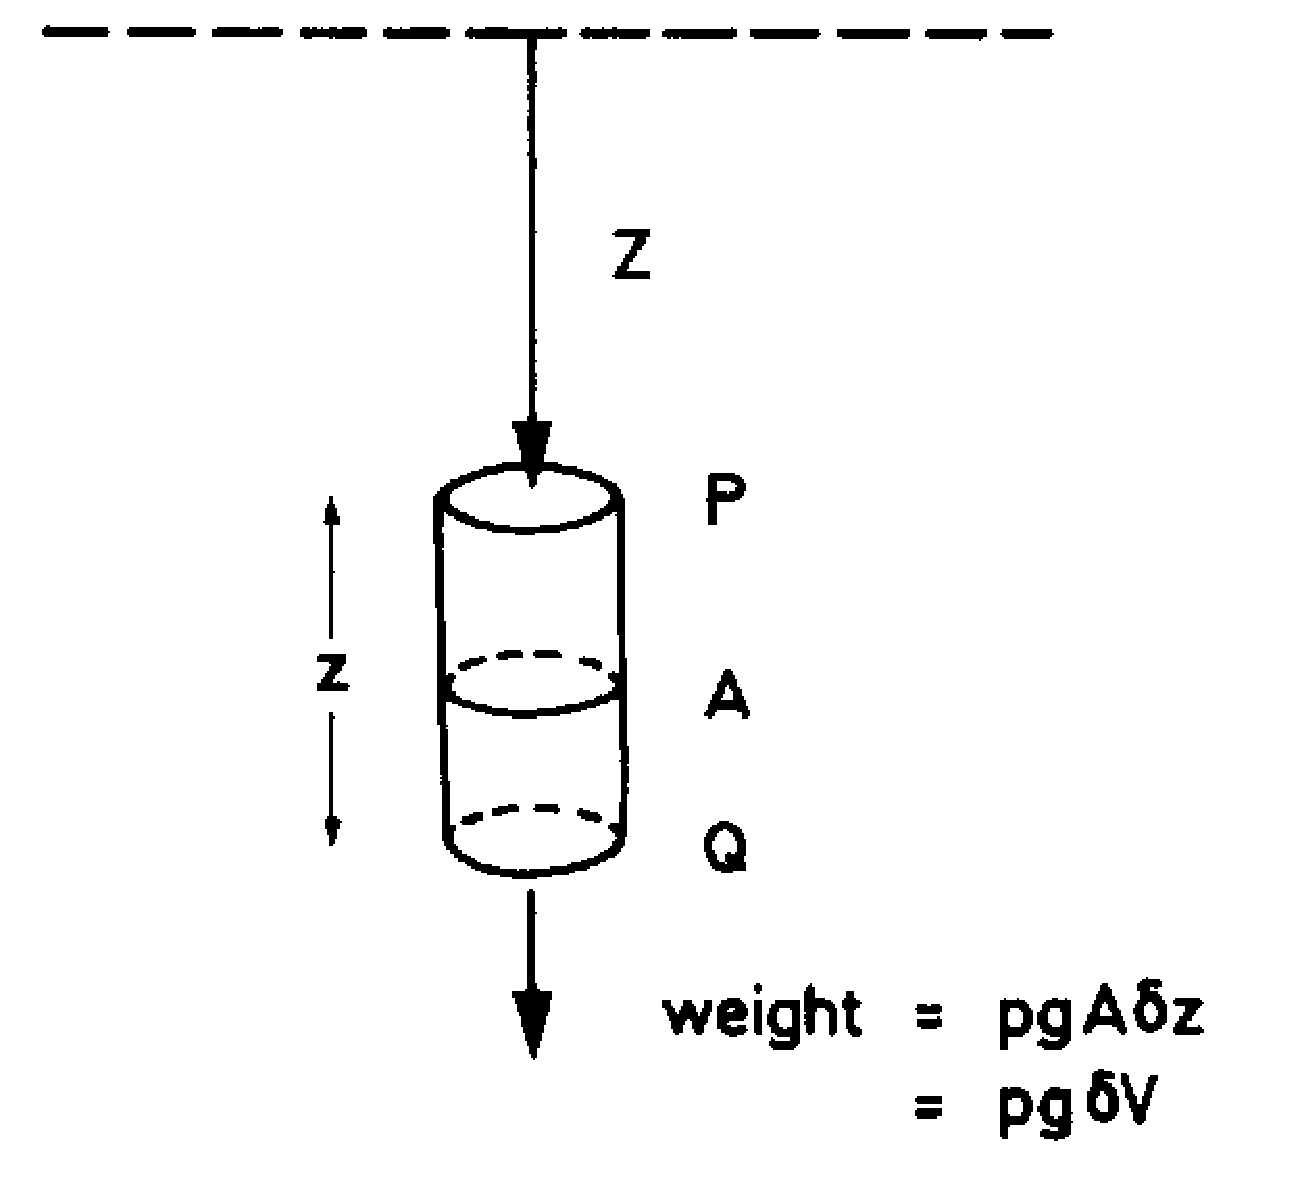
\includegraphics[width=2.5in]{Section27.pdf}}
\label{fig7}
\end{wrapfigure}

For a vertical cylindrical element at rest in equilibrium under the action 
of pressure thrusts and the weight of fluid
\[-{{\bf k}}. \nabla p\delta V+\rho g\delta 
V=0,\]
 where ${{\bf k}}=(0,0,1)$.

Thus ${dp}/{dz}=\rho g$, per unit volume, since $p = 
p(z)$ only [otherwise we would write $\partial p/\partial z$].
Hence $\rho ={\left( {{dp}/ {dz}} \right)} / g$ is a function of $z$ at most, i.e., $\rho  = 
\rho (z)$. Here $z$ measures downwards so that $\hbox{sgn} (\delta z) = \hbox{sgn} 
(\delta p)$. Normally we take $z$ upwards whereupon
\[
\frac{dp}{dz}=-\rho g.
\]
(Show this.) The equation above is generally called the \textbf{hydrostatic 
equation}.

\subsection{Liquids and gases}
Liquids undergo little change in volume with pressure over a very large 
range in pressure and it is frequently a good assumption to assume that 
$\rho $ = constant (which is the definition of a homogeneous fluid). In that 
case, the foregoing equation (with $z$ pointing downwards) integrates to give
\[
p=p_0 +\rho gz ,
\]
where $p = p_{0}$ at the level $z = 0$.

Ideal gases are such that pressure, density and temperature are related 
through the ideal gas equation, $p = \rho RT$, where $T$ is the absolute 
temperature and $R$ is the specific gas constant. If a certain volume of gas 
is isothermal (i.e., has constant temperature), then pressure and density 
vary exponentially with depth with a so-called \textbf{e-folding} scale 
$H_{s} = RT/g$ (see exercises).

\begin{wrapfigure}{r}{2.5in}
\centerline{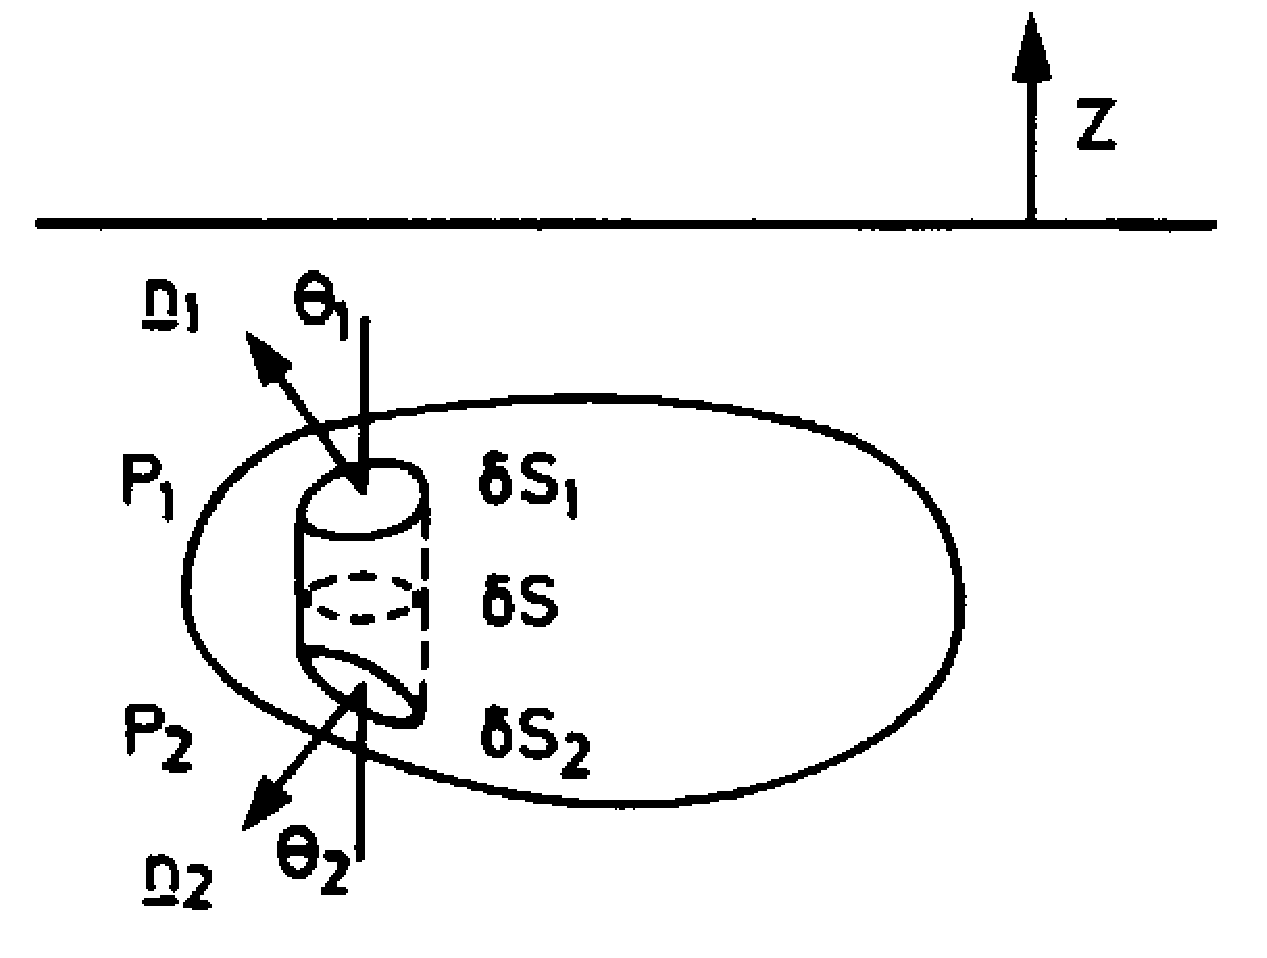
\includegraphics[width=2.5in]{Section28.pdf}}
\label{fig8}
\end{wrapfigure}

\subsection{Archimedes Principle}
In a fluid at rest the net pressure gradient force per unit volume acts 
vertically upwards and is equal to $-dp/dz$ (when $z$ points upwards) and the 
gravitational force per unit volume is $\rho g$. Hence, for equilibrium, 
$dp/dz = -\rho g$. 

Consider the vertically-oriented cylindrical element $P_{1} P_{2}$ of an 
immersed body in equilibrium, which intersects the surface of the body to 
form surface elements $\delta S_{1}$ and $\delta S_{2}$ which have 
normals $\textbf{n}_{1}$, $\textbf{n}_{2}$ inclined at angles $\theta _1$,
$\theta _2 $ to the vertical. The net upward thrust on these small 
surfaces is:
\[
\hbox{Thrust} =p_2 \cos \theta _2 \delta S_2 -p_1 \cos \theta _1 
\delta S_1 =(p_2 -p_1 )\delta S\quad ,
\]
where $\delta S_{1} \cos \theta _{1 }=\delta S_{2} \cos \theta 
_{2}=\delta S$ is the horizontal cross-sectional area of the cylinder. 

Since, $p_2 -p_1 =-\int_{z_1 }^{z_2 } {\rho gdz} $,
the net upward thrust is:
\[\hbox{Thrust}=\left( {\int_{z_2 }^{z_1 } {\rho gdz} } 
\right)\delta S = \hbox{weight of liquid displaced}. \]

If this integration is now continued over the whole body we obtain one 
version of \textbf{Archimedes Principle} which states that the resultant 
thrust on an immersed body in equilibrium has magnitude equal to the weight 
of fluid displaced and acts upward through the centre of mass of the 
displaced fluid (provided that the gravitational field is uniform).

\section{Equation of Motion for an inviscid fluid}
If we apply Newton's second law to a unit volume of fluid:
\begin{description}
\item[(i)] the mass of the element is $\rho $ kg m$^{-3}$ ;
\item[(ii)] the acceleration must be that \textbf{following the fluid element} to 
take account both of the change in velocity with time at a fixed point and 
of the change with position of the velocity field at a fixed time,
\[
\frac{D{{\bf u}}}{Dt}=\frac{\partial {{\bf u}}}{\partial 
t}+({{\bf u}}. \nabla ){{\bf 
u}}=\frac{\partial {{\bf u}}}{\partial 
t}+u\frac{\partial {{\bf u}}}{\partial 
x}+v\frac{\partial {{\bf u}}}{\partial 
y}+w\frac{\partial {{\bf u}}}{\partial z};
\]
\item[(iii)] the total force acting on the element (neglecting viscosity or fluid 
friction) comprises the contact force acting across the surface of the 
element -$\nabla p$ per unit volume, which is a \textbf{pressure gradient 
force} arising from the difference in pressure across the element, and any 
body forces \textbf{F}, acting throughout the fluid including especially the 
gravitational weight per unit volume, $-g\rho \textbf{k}$.
\end{description}

The resulting \textbf{equation of motion} or \textbf{momentum equation} for 
inviscid fluid flow, known as \textbf{Euler's equation}, is
\begin{alignat*}{4}
& \frac{\partial u}{\partial t} & +
& \left( {{{\bf u}}. \nabla } \right){{\bf u}}  & =
& -\frac{1}{\rho }\nabla p & + &\  \textbf{F} , \\
&\hbox{(A)}&
&\ \ \ \hbox{(B) }&
&\ \ \ \ \hbox{(C)}&
&\hbox{(D)}\end{alignat*}
where (A) --- local acceleration, (B) --- advective acceleration, (C) ---
pressure gradient force and (D) --- body force.

In rectangular cartesian coordinates $(x,y,z)$ with velocity components 
$(u,v,w)$ the component equations are 
\begin{align*}
&\frac{\partial u}{\partial t}+u\frac{\partial u}{\partial 
x}+v\frac{\partial u}{\partial y}+w\frac{\partial 
u}{\partial z}=-\frac{1}{\rho }\frac{\partial p}{\partial 
x}+X, \\
& \frac{\partial v}{\partial t}+u\frac{\partial v}{\partial 
x}+v\frac{\partial v}{\partial y}+w\frac{\partial 
v}{\partial z}=-\frac{1}{\rho }\frac{\partial p}{\partial 
y}+Y, \\
& \frac{\partial w}{\partial t}+u\frac{\partial w}{\partial 
x}+v\frac{\partial w}{\partial y}+w\frac{\partial 
w}{\partial z}=-\frac{1}{\rho }\frac{\partial p}{\partial 
z}+Z
\end{align*}
where $ \textbf{F} = (X,Y,Z)$ is the external force per unit mass (or body 
force). These are \textbf{three} partial differential equations in the 
\textbf{four} dependent variables $u$, $v$, $w$, $p$ and four independent variables 
$x$, $y$, $z$, $t$. For a complete system we require \textbf{four} equations in the 
four variables, and the extra equation is the conservation of mass or 
\textbf{continuity equation,} which for an incompressible fluid has the form
\[
\nabla . {\bf u}=0\quad\hbox{or} \quad \frac{\partial 
u}{\partial x}+\frac{\partial v}{\partial y}+\frac{\partial 
w}{\partial z}=0\quad .
\]
There is no equivalent to the continuity equation in either particle or 
rigid body mechanics, because in general mass is permanently associated with 
bodies. In fluids, however, we must ensure that holes do not appear or that 
fluid does not double up, and we do this by requiring that $\nabla . 
{\bf u}=0$ which implies that in the absence of sources or sinks there can be no 
net flow either into or out of any closed surface. We may regard this as a 
geometric condition on the flow of an incompressible fluid. It is not, of 
course, satisfied by a compressible fluid (c.f. a bicycle pump). We say that 
any incompressible flow satisfying the continuity equation $\nabla . 
{{\bf u}}=0$ is a \textbf{kinematically possible motion}. 

The Euler equation plus continuity equation are extremely important but 
extremely difficult to solve. With possible further force terms on the 
right, they represent the behaviour of gaseous stars, the flow of oceans and 
atmosphere, the motion of the earth's mantle, blood flow, air flow in the 
lungs, many processes of chemistry and chemical engineering, the flow of 
water in rivers and in the permeable earth, aerodynamics of aeroplanes, and 
so forth.

The difficulty of solution, and there are probably no more than a dozen or 
so solutions known for very simple geometries, arises from the 
\textbf{non-linear} term $({\bf u}. \nabla ){\bf u}$ as a result of which if 
\textbf{u}$_{1}$ and \textbf{u}$_{ 2}$ are two solutions of the equation 
$c_{1 }\textbf{u}_{ 1} + c_{2 }\textbf{u}_{ 2}$ (where $c_{1 }$ and 
$c_{2}$ are constants) is in general \textit{not} a solution, so that we lose one of our 
main methods of solution.

\begin{exmp}
Suppose that the velocity field is ${{\bf u}}=(-\Omega 
y,\Omega x,0)$ for $\Omega $ constant. Show that it is a 
kinematically possible flow for an incompressible liquid in a uniform 
gravitational field $F\equiv g=(0,0,-g)$. Determine the corresponding 
pressure field.
\end{exmp}

%\textbf{Solution}

%(i) This is a \textbf{kinematically possible} steady incompressible flow, as 
%\textbf{u} satisfies the continuity equation
%\[
%\nabla . {{\bf u}}=\frac{\partial u}{\partial 
%x}+\frac{\partial v}{\partial y}+\frac{\partial w}{\partial 
%z}=0+0+0=0.
%\]
%(ii) We find the corresponding pressure field from Euler's equation
%\[
%{{\bf u}}. \nabla {{\bf u}}=-\frac{1}{\rho }\nabla 
%p-g{{\bf k}}.
%\]
%If the given velocity field is substituted in the Euler's equation and it is 
%rearranged in component form,
%\[
%\frac{\partial p}{\partial x}=\rho \Omega ^2x,\frac{\partial 
%p}{\partial y}=\rho \Omega ^2y,\frac{\partial p}{\partial 
%z}=-\rho g.
%\]
%We may now solve these three equations as follows.

%$\frac{\partial p}{\partial x}\equiv \left( {\frac{\partial 
%p}{\partial x}} \right)_{y,z\mbox{constant}} =\rho \Omega 
%^2x\Rightarrow p=\textstyle{1 \over 2}\rho \Omega 
%^2x^2+$constant

%where "constant" can include arbitrary functions of both y and z (Check: 
%$\partial p/\partial x=\rho \Omega ^2x+0)$. We continue in 
%like manner with the other component equations:
%\[
%\frac{\partial p}{\partial y}=\rho \Omega 
%^2y\Rightarrow 
%p=\textstyle{1 \over 2}\rho \Omega 
%^2y^2+g(z,x)
%\]
%\[
%\frac{\partial p}{\partial z}=-\rho g 
%\Rightarrow p=-\rho gz+h(x,y),
%\]
%where f$(y,z)$, g$(z,x)$ and h$(x,y)$ are \textbf{arbitrary functions}. By 
%comparison of the three solutions we see that f$(y,z)$ must incorporate 
%$\textstyle{1 \over 2}\rho \Omega ^2y^2$ and -$\rho $gz and so forth. 
%Hence the full solution is

%$p=\textstyle{1 \over 2}\rho \Omega 
%^2(x^2+y^2)-\rho gz+$ constant ,

%and we find that this solution does in fact satisfy each of the component 
%Euler equations. On a free surface containing the origin O (x = 0, y = 0, z 
%= 0), p = p$_{o} \quad \Rightarrow $ the constant = p$_{o}$, where p$_{o}$ is 
%atmospheric pressure, and r$^{2}$ = x$^{2}$ + y$^{2}$,
%\[
%p=p_0 +\textstyle{1 \over 2}\rho \Omega ^2r^2-\rho 
%gz\quad .
%\]
%(iii) The equation for the free surface is now given by p = p$_{0}$ over the 
%whole liquid surface, which therefore has equation
%\[
%z=\frac{\rho \Omega ^2}{2\rho g}r^2=\frac{\Omega 
%^2}{2g}r^2\quad .
%\]
%(iv) Streamlines in flow are given by

%$\frac{dx}{u}=\frac{dy}{v}=\frac{dz}{w}$ or 
%$\frac{dx}{-\Omega y}=\frac{dy}{\Omega x}=\frac{dz}{0}$

%yielding two relations

%$\int {\Omega xdx+\int {\Omega 
%ydy=0\Rightarrow } } $ x$^{2}$ + y$^{2}$ = 
%constant
%\[
%\int 
%{dz=0 
%\Rightarrow 
%z=\mbox{const}} 
%ant,
%\]
%and streamlines are circles about the z-axis in planes z = constant. The 
%velocity field represents rigid body rotation of fluid with angular velocity 
%$\Omega $ about the axis 0z (imagine a tin of water on turntable).

\section{Equations of motion in cylindrical polars}

\begin{wrapfigure}{r}{2.5in}
\centerline{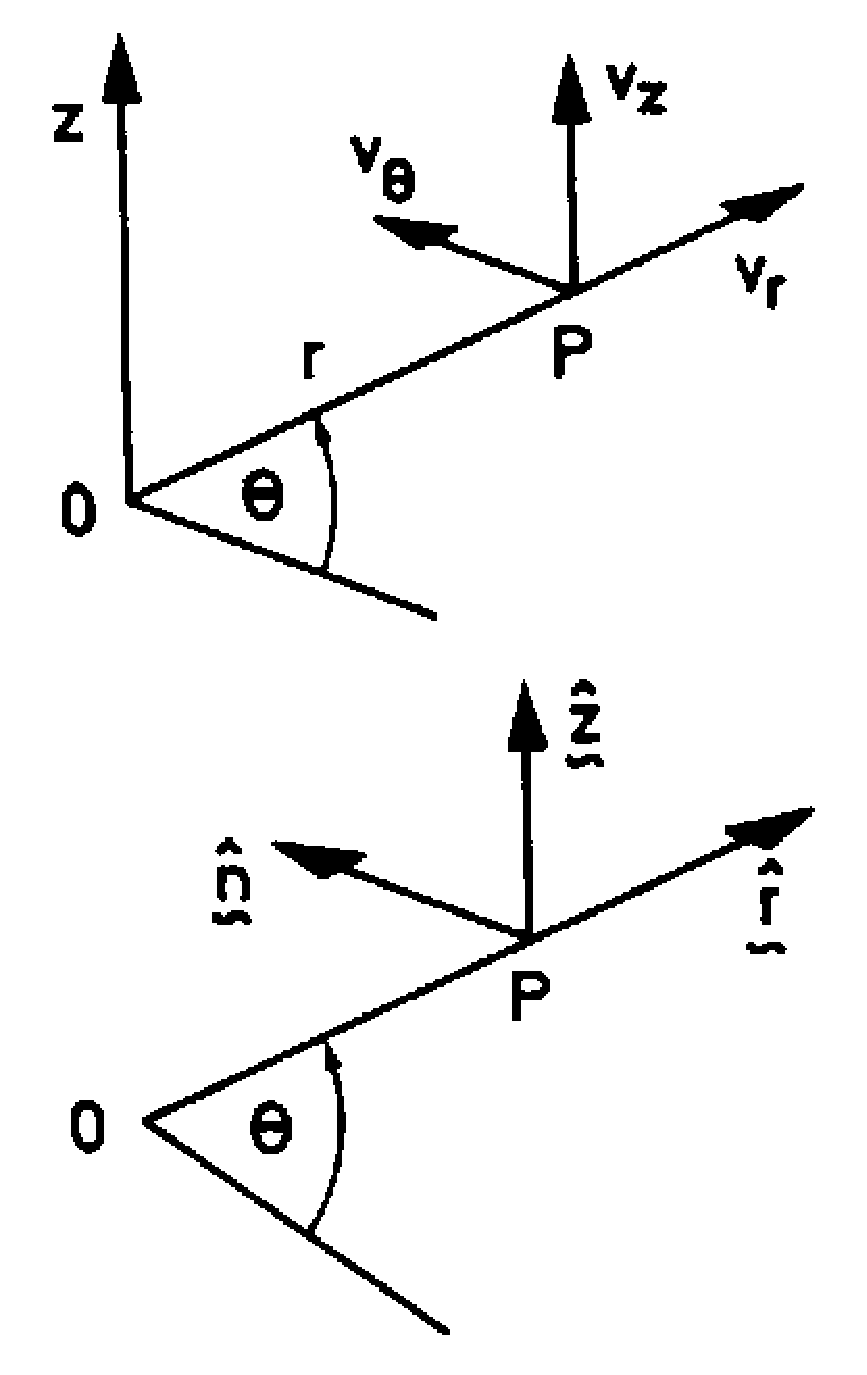
\includegraphics[width=2.5in]{Section29.pdf}}
\label{fig9}
\end{wrapfigure}

Take the cylindrical polars $(r,\theta,z)$ and velocity 
$(v_r ,v_\theta ,v_z )$. This is more complicated than rectangular 
cartesians as $v_{r}$, and $v_{\theta }$ change in direction with $P$ (in fact 
$0P$ rotates about $0z$ with angular velocity $v_{\theta }/r$). Suppose that 
${\bf \hat {r}}, {\bf \hat {n}}, {\bf \hat {k}}$ are 
the unit vectors at $P$ in the radial, azimuthal and axial directions, as 
sketched. Then ${\bf \hat {k}}$ is fixed in direction (and, of course, 
magnitude) but ${\bf \hat {r}}$ and ${\bf \hat {n}}$ rotate in 
the plane $z = 0$ as $P$ moves, and it follows that $d{\bf \hat {k}}/dt = 
\textbf{0}$, but that
\[
\frac{d}{dt}{{\bf \hat {r}}}={{\bf \dot {\hat 
{r}}}}={{\bf \hat {n}}}\dot {\theta }, {{\bf \dot 
{\hat {n}}}}=(-{{\bf \hat {r}}})\dot {\theta 
}=-{{\bf \hat {r}}}\dot {\theta }
\]
Hence, as $\dot {\theta }=v_\theta /r$,
\begin{align*}
& {{\bf v}}=(v_r {{\bf \hat {r}}}+v_\theta {{\bf 
\hat {n}}}+v_z {{\bf \hat {k}}}), \\
& {{\bf \dot {v}}}=\dot {v}_r {{\bf \hat {r}}}+v_r 
{{\bf \dot {\hat {r}}}}+\dot {v}_\theta {{\bf \hat 
{n}}}+v_\theta {{\bf \dot {\hat {n}}}}+\dot {v}_z {\rm 
{\bf \hat {k}}} \\
& \phantom{{{\bf \dot {v}}}} =(\dot {v}_r -v_\theta ^2 /r){{\bf \hat 
{r}}}+(\dot {v}_\theta +v_r v_\theta /r){{\bf \hat 
{n}}}+\dot {v}_z {{\bf \hat {k}}}.
\end{align*}
Recalling also that $d/dt$ must be interpreted here as $D/Dt$, the acceleration 
is
\[
\left[ {\frac{Dv_r }{Dt}-\frac{v_\theta ^2 }{r},\frac{Dv_\theta 
}{Dt}+\frac{v_r v_\theta }{r},\frac{Dv_z }{Dt}} \right]\quad .
\]
If we now write $(u,v,w)$ in place of $(v_{r} ,v_{\theta } ,v_{z} )$, 
Euler's equations in cylindrical polar coordinates take the form
\begin{align*}
&
\frac{\partial u}{\partial t}+u\frac{\partial u}{\partial 
r}+\frac{v}{r}\frac{\partial u}{\partial \theta 
}+w\frac{\partial u}{\partial 
z}-\frac{v^2}{r}=-\frac{1}{\rho }\frac{\partial 
p}{\partial r}+F_r ,
\\
&
\frac{\partial v}{\partial t}+u\frac{\partial v}{\partial 
r}+\frac{v}{r}\frac{\partial v}{\partial \theta 
}+w\frac{\partial v}{\partial z 
}+\frac{uv}{r}=-\frac{1}{\rho r}\frac{\partial 
p}{\partial \theta }+F_\theta ,
\\
&
\frac{\partial w}{\partial t}+u\frac{\partial w}{\partial 
r}+\frac{v}{r}\frac{\partial w}{\partial \theta 
}+w\frac{\partial w}{\partial z}=-\frac{1}{\rho 
r}\frac{\partial p}{\partial z}+F_z , \\
& \frac{1}{r}\frac{\partial \left( {ru} \right)}{\partial 
r}+\frac{1}{r}\frac{\partial v}{\partial \theta 
}+\frac{\partial w}{\partial z}=0
\\
\end{align*}

\section{Dynamic or perturbation pressure}

If in the Euler equation for an incompressible fluid,
\begin{equation}
\label{eq22}
\frac{D{{\bf u}}}{Dt}=-\frac{1}{\rho }\nabla p+{\rm 
{\bf g}}\quad ,
\end{equation}
we put ${\bf u}=0$ to represent the equilibrium or rest state,
\begin{equation}
\label{eq23}
{{\bf 0}}=-\frac{1}{\rho }\nabla p_0 +{{\bf g}}
\end{equation}
This is merely the hydrostatic equation 
\[
\nabla p_0 =\rho {{\bf g}}\quad \mbox{or}\quad \frac{\partial 
p_0 }{\partial x}=0,\frac{\partial p_0 }{\partial 
y}=0,\frac{\partial p_0 }{\partial z}=\rho g
\]
where $p_0$ is the hydrostatic pressure. Subtracting (\ref{eq22}) - (\ref{eq23}) we 
obtain
\[
\frac{D{{\bf u}}}{Dt}=-\frac{1}{\rho }\nabla (p-p_0 
)=-\frac{1}{\rho }\nabla p_d 
\]
where $p_{d} = p - p_{0}$ = (total pressure) - (hydrostatic pressure) is 
known as the \textbf{dynamic pressure} (or sometimes, especially in 
dynamical meteorology, the perturbation pressure). The dynamic pressure is 
the excess of total pressure over hydrostatic pressure, and is the only part 
of the pressure field associated with motion.

We shall usually omit the suffix $d$ since it is fairly clear that if 
\textbf{g} is included we are using \textbf{total} pressure, and if no 
\textbf{g} appears we are using the dynamic pressure,
\[
\frac{D{{\bf u}}}{Dt}=\frac{\partial {{\bf u}}}{\partial 
t}+({{\bf u}}. \nabla ){{\bf 
u}}=-\frac{1}{\rho }\nabla p\quad .
\]

\section{Incompressible viscous fluids}

It can be shown that the viscous (frictional) forces in a fluid may be 
expressed as $\mu \nabla ^2{\bf u}=\rho \nu \nabla ^2{\bf u}$ where \textit{$\mu $} the 
\textbf{coefficient of viscosity} and $\nu =\mu /\rho $ the 
\textbf{kinematic viscosity} provide a measure of the magnitude of the 
frictional forces in particular fluid, i.e., $\mu $ and $\nu $ are 
properties of the fluid and are relatively small in air or water and large 
in glycerine or heavy oil.

In a viscous fluid the equation of motion for unit mass,
\begin{alignat*}{5}
& \frac{\partial {\bf u}}{\partial t} & +
& \left( {{{\bf u}}. \nabla } \right){{\bf u}}  & =
& -\frac{1}{\rho }\nabla p & + &\  \textbf{F} & + &\nu \nabla ^2{\bf u}, \\
&\hbox{(A)}&
&\ \ \ \hbox{(B) }&
&\ \ \ \ \hbox{(C)}&
&\hbox{(D)}&
&\ \ \hbox{(E)} 
\end{alignat*}
is known as the \textbf{Navier-Stokes' equation}. The various terms are: (A)
--- local acceleration, (B) --- advective acceleration, (C) --- pressure
gradient force, (D) --- body force, and (E) --- viscous force.

The viscous term is small relative to other terms except close to 
boundaries, yet it contains the highest order derivatives $(\partial_x ^2{\rm 
{\bf u}},\partial_y ^2{{\bf u}},\partial_z ^2{{\bf u}})$, and hence determines the 
number of spatial boundary conditions that must be imposed to determine a 
solution.

We require also the continuity equation,
\[
\nabla . {\bf u}=0,
\]
to close the system of four differential equations in four dependent 
variables.

The Navier-Stokes equation is too difficult for us to handle at present and 
we shall concentrate on Euler's equation from which we can learn much about 
fluid flow. Euler's equation is still non-linear, but there are clever 
methods to bypass this difficulty. 

\section{Boundary conditions for fluid flow}
\begin{description}
\item[(i)] \textbf{Solid boundaries}: there can be no normal component of velocity 
(through the boundary). If friction is neglected there may be free slip 
along the boundary, but friction has the effect of slowing down fluid near 
the boundary and it is observed experimentally that there is no relative 
motion at the boundary, either normal or tangential to the boundary. In 
fluids with low viscosity this tangential slowing down occurs in a thin 
\textbf{boundary layer}, and in a number of important applications this 
boundary layer is so thin that it can be neglected and we can say 
approximately that the fluid slips at the surface; in many other cases the 
entire boundary layer separates from the boundary and the inviscid model is 
a very poor approximation.

Thus, in an inviscid flow (also called an ideal fluid) the fluid velocity 
must be tangential at a rigid body, and: 
\begin{itemize}
\item for a surface at rest ${{\bf n}}. {{\bf u}}={\rm 
{\bf 0}}$;
\item for a surface with velocity $\textbf{ u}_{s }$ then ${{\bf n}}. 
\left( {{{\bf u}}-{{\bf u}}_s } \right)={{\bf 0}}$ .
\end{itemize}
\item[(ii)] \textbf{Free boundaries}: at an interface between two fluids (of which 
one might be water and one air) the pressure must be continuous, or else 
there would be a finite force on an infinitesimally small element of fluid 
causing unbounded acceleration; and the component of velocity 
\textbf{normal} to the interface must be continuous. If viscosity is 
neglected the two fluids may slip over each other. If there is liquid under 
air, we may take $ p = p_{0}  = $atmospheric pressure at the interface, where 
$p_{0}$ is taken as constant. If surface tension is important there may be a 
pressure difference across the curved interface. 
\end{description}

\subsection{An alternative boundary condition}
As the velocity at a boundary of an \textbf{inviscid fluid} must be wholly 
tangential, it follows that a fluid particle once at the surface must always 
remain at the surface. Hence for a surface or boundary with equation
\[
F(x,y,z,t)=0\quad ,
\]
if the coordinates of a fluid particle satisfy this equation at one instant, 
they must satisfy it always. Hence, moving with the fluid at the boundary,
\[
\frac{DF}{Dt}=0
\]
or 
\[ \frac{\partial F}{\partial t}+{{\bf u}}. \nabla 
F=0, \]
as F must remain zero for all time for each particle at the surface.

\subsection*{Exercises}
\begin{enumerate}
\item Under what condition is the advective rate-of-change equal to the total 
rate-of-change?

\item Express ${\bf u}. \nabla$ and $\nabla . {\bf u}$ in cartesian form and show 
they are quite different, one being a scalar function and one a scalar 
differential operator.

\item The vector differential operator del (or nabla) is defined as
\[
\nabla =\left( {\frac{\partial }{\partial x},\frac{\partial }{\partial 
y},\frac{\partial }{\partial z}} \right)
\]
in rectangular cartesian coordinates. Express in full cartesian form the 
quantities: $\nabla . {\bf u}$, $\nabla \times {\bf u}$, ${\bf u}. \nabla $
,$\nabla . \nabla $, and identify each.

\item Show that 
\[\frac{\partial }{\partial x}\left( {\frac{Df}{Dt}} 
\right)=\frac{Df}{Dt}+\frac{\partial {{\bf u}}}{\partial x}. \nabla 
f. \]

\item Show that when in hydrostatic equilibrium, the pressure and density in an 
isothermal (i.e., constant temperature) atmosphere vary with height 
according to the formulae 
\[ p(z)=p(0)\exp (-z/H_s ) \quad \hbox{and}\quad \rho (z)=\rho 
(0)\exp (-z/H_s ). \]
 where $H_s ={RT/ g}$ and $z$ points vertically upwards. Show 
that for realistic values of $T$ in the troposphere and $R=287 \hbox{ J
K}^{-1}\hbox{kg}^{-1}$, the e-folding height
scale $H_{s}$ is on the order of 8 km.

\item You are on a small raft floating in a pool, and you throw a heavy anchor 
overboard. Does the water level of the pool rise, fall or remain the same? 
Carefully justify your answer.

\item Is the velocity field ${{\bf u}}=\left( {\cos x,xz^2,z\sin x} 
\right)$ kinematically possible? Why?

\item Find the pressure field in the inviscid, incompressible flow with 
velocity field ${{\bf u}}=\left( {kx,-ky,0} \right)$, where $k$ is a 
constant.

\item Show that ${{\bf \dot {\hat {r}}}}={{\bf \hat 
{n}}}\dot {\theta }$ and ${{\bf \dot {\hat {n}}}}=-{{\bf 
\hat {r}}}\dot {\theta }$.

\item Show that the continuity equation in cylindrical polar coordinates is
\[
\frac{1}{r}\frac{\partial \left( {ru} \right)}{\partial 
r}+\frac{1}{r}\frac{\partial v}{\partial \theta 
}+\frac{\partial w}{\partial z}=0.
\]
\end{enumerate}

\cleardoublepage


\chapter{Steady Inviscid Flows}

\section{Bernoulli's equation}
For steady inviscid flow under external forces which have a potential 
$\Omega $ such that ${{\bf F}}$=-$\nabla \Omega $ the Euler equation 
reduces to
\[
\left( {{{\bf u}}. \nabla } \right){{\bf 
u}}=-\frac{1}{\rho }\nabla p-\nabla \Omega \quad ,
\]
and for incompressible fluids
\[
\left( {{{\bf u}}. \nabla } \right){{\bf 
u}}+\frac{1}{\rho }\nabla (p+\rho \Omega )={{\bf 
0}}\quad .
\]
We may regard $p + \rho \Omega $ as a more general \textbf{dynamic 
pressure}; but for the particular case of gravitation potential, $\Omega  = 
gz$, and ${{\bf F}}=-\nabla \Omega 
=-(0,0,g)=-g{{\bf k}}$.

We note that
\begin{align*}
{{\bf u}}. ({{\bf u}}. \nabla ){{\bf 
u}} & =u({{\bf u}}. \nabla )u+v({{\bf 
u}}. \nabla )v+w({{\bf u}}. \nabla )w
\\\
&
={{\bf u}}. \nabla \textstyle{1 \over 
2}(u^2+v^2+w^2)
\\
&
=({{\bf u}}. \nabla )\textstyle{1 \over 2}{{\bf u}}^2
\end{align*}
using the fact that $\textbf{u}.  \nabla $ is a scalar differential 
operator. Hence,
\[
{{\bf u}}. \left[ {\left( {{{\bf u}}. \nabla } 
\right){{\bf u}}+\frac{1}{\rho }\nabla \left( {p+\rho 
\Omega } \right)} \right]={{\bf u}}. \nabla \left( 
{{1 \over 2}{{\bf u}}^2+\frac{p}{\rho }+\Omega 
} \right)=0\quad ,
\]
and it follows that $(\textstyle{1 \over 2}{{\bf u}}^2+p / 
\rho +\Omega )$ is constant along each streamline (as \textbf{u}$. 
\nabla $ is the derivative in the direction \textbf{u}, and hence 
proportional to the rate of change in the direction \textbf{u} of 
streamlines).

Thus for steady, incompressible, inviscid flow, Bernoulli's equation states
\[ {1 \over 2}{{\bf u}}^2+\frac{p}{\rho 
}+\Omega \quad = \hbox{constant on a streamline}, \]
although the constant will generally be different on each different 
streamline.

\section{Applications of Bernoulli's equation}

\begin{wrapfigure}{r}{2.5in}
\centerline{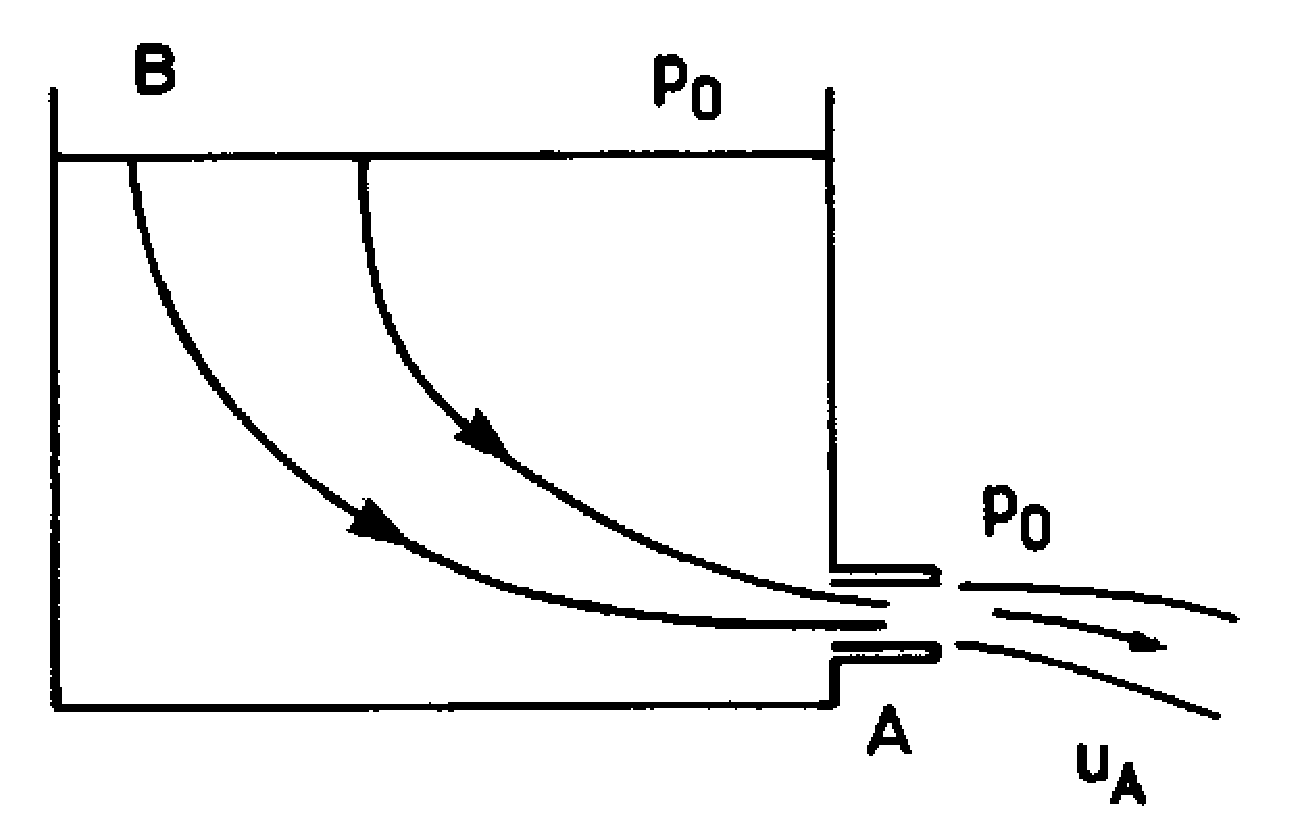
\includegraphics[width=2.5in]{Section31.pdf}}
\label{fig1}
\end{wrapfigure}

\subsection{Draining a reservoir through a small hole}
If the draining opening is of much smaller cross-section than the reservoir, 
the water surface in the tank will fall very slowly and the flow may be 
regarded as approximately steady. We may take the outflow speed $u_{A}$ as 
approximately uniform across the jet and the pressure $p_{A}$ uniform across 
the jet and equal to the atmospheric pressure $p_{0}$ outside the jet (for, 
if this were not so, there would be a difference in pressure across the 
surface of the jet, and this would accelerate the jet surface radially, 
which is not observed, although the jet is accelerated downwards by its 
weight). Hence, on the streamline $AB$,
\[
{1 \over 2}u_A^2 +\frac{p_0 }{\rho }=\textstyle{1 
\over 2}u_B ^2+\frac{p_0 }{\rho }+gh\quad ,
\]
and as $u_{B} \ll u_{A }$ then $u_A =\sqrt {2gh} $ .

This is known as Toricelli's theorem. Note that the outflow speed is that of 
free fall from $B$ under gravity; this clearly neglects any viscous 
dissipation of energy.

\subsection{Bluff body in a stream; Pitot tube}
\begin{wrapfigure}{r}{3in}
\centerline{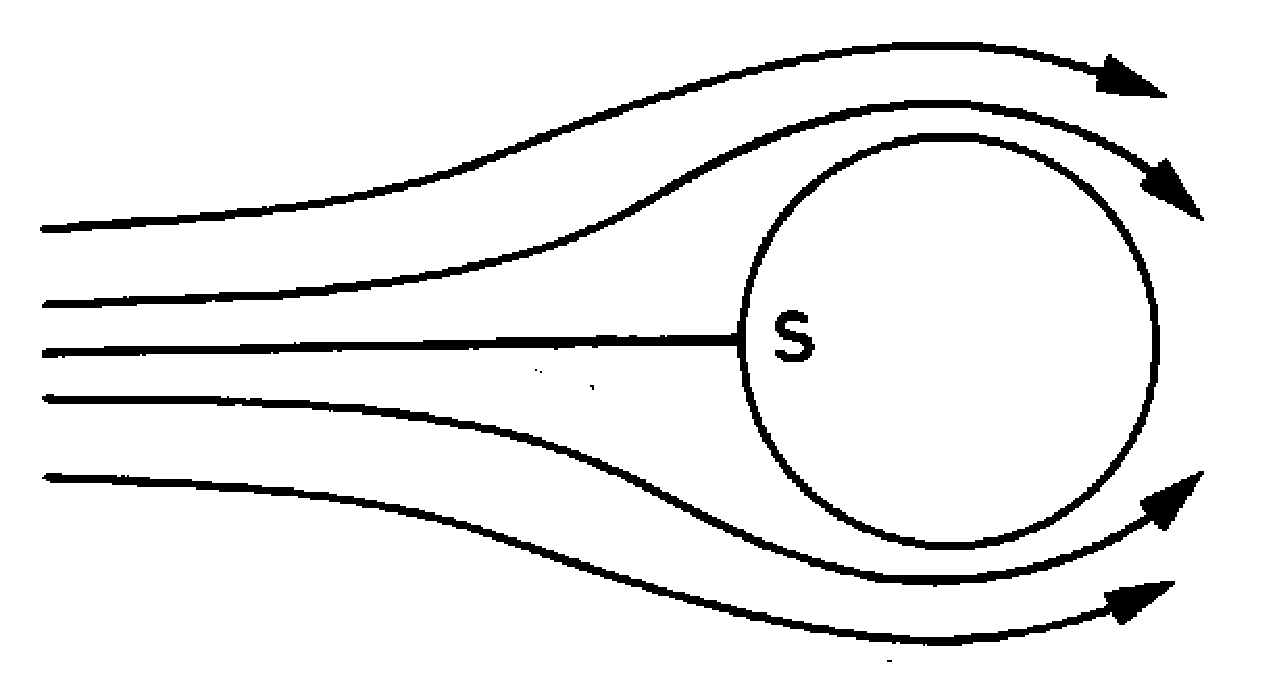
\includegraphics[width=3in]{Section32.pdf}}
\label{fig2}
\end{wrapfigure}

Suppose that a stream has uniform speed $U_{0}$ and pressure $p_{0}$ far 
from any obstacle, and that it then flows round a bluff body. The flow must 
be slowed down in front of the body and there must be one \textbf{dividing 
streamline} separating fluid which follows past one side of the body or the 
other. This dividing streamline must end on the body at a \textbf{stagnation 
point} at which the velocity is zero and the pressure
\[
p=p_0 +{1 \over 2}\rho U_0^2 .
\]

\begin{wrapfigure}{r}{3in}
\centerline{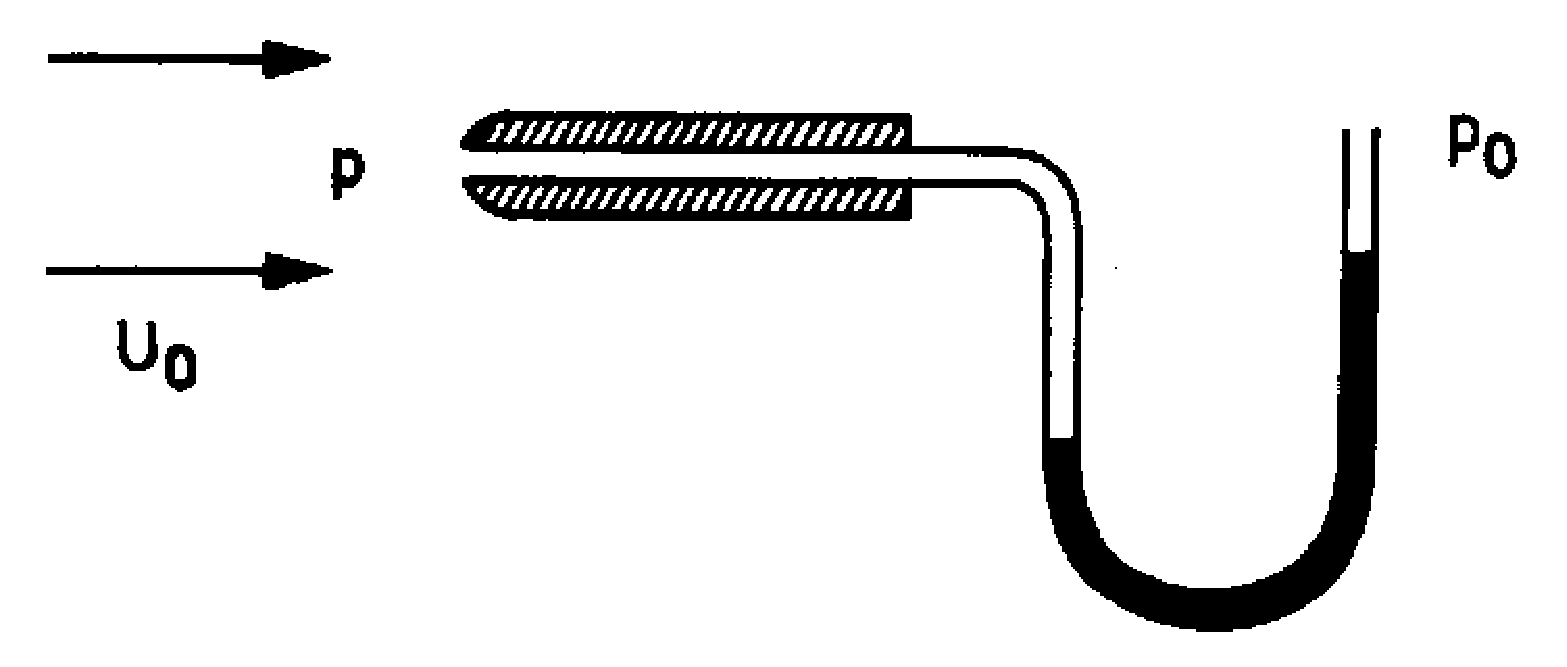
\includegraphics[width=3in]{Section33.pdf}}
\label{fig3}
\end{wrapfigure}

This provides the basis for the Pitot tube in which a pressure measurement 
is used to obtain the free stream velocity $U_{0}$. The pressure 
$p=p_0 +\textstyle{1 \over 2}\rho U_0^2 $ is the 
\textbf{total} or \textbf{Pitot pressure} (also known as the \textbf{total 
head}) of the free stream, and differs from the static pressure $p_{0}$ by 
the dynamic pressure $\textstyle{1 \over 2}\rho U_0^2 $. The Pitot tube 
consists of a tube directed into the stream with a small central hole 
connected to a \textbf{manometer} for measuring pressure difference $p - 
p_{0}$ . At equilibrium there is no flow through the tube, and hence the 
left hand pressure on the manometer is the total pressure $p_0 
+\textstyle{1 \over 2}\rho U_0^2 $. The static pressure $p_{0}$ can 
be obtained from a \textbf{static tube} which is normal to the flow.

\subsection*{Exercises}

\begin{enumerate}

\item Prove the vector identity
\[
\nabla \left( {{{\bf a}}. {{\bf b}}} \right)=\left( {{{\bf 
b}}. \nabla } \right){{\bf a}}+\left( {{{\bf a}}. \nabla } 
\right){{\bf b}}+{{\bf b}}\times \left( {\nabla \times {{\bf 
a}}} \right)+{{\bf a}}\times \left( {\nabla \times {{\bf b}}} 
\right).
\]
Hence show that 
\[
\left( {{{\bf u}}. \nabla } \right){{\bf u}}=\nabla \left( 
{\textstyle{1 \over 2}{{\bf u}}^2} \right)-{{\bf u}}\times \left( 
{\nabla \times {{\bf u}}} \right)=\nabla \left( {\textstyle{1 \over 
2}{{\bf u}}^2} \right)-{{\bf u}}\times {\bm\omega},
\]
where $ {\bm\omega}=\nabla \times {{\bf u}}$ is known as the \textbf{vorticity}.

\item Hold two sheets of paper at $A$ and $B$ with a finger between the two at top 
and bottom, and blow between the sheets as illustrated below. The trailing edges 
of the sheets will not move apart as you might have anticipated, but 
together. Explain this in terms of Bernoulli's equation, assuming the flow 
to be steady.

\item Explain why there is an increase in pressure on the side of a building 
facing the wind.

\item A uniform straight open rectangular channel carries a water flow of mean 
speed $U$ and depth $h$. The channel has a constriction, which reduces its width 
by half and it is observed that the depth of water in the constriction is 
only $\textstyle{1 \over 2}h$. By applying Bernoulli's theorem to a surface 
streamline find $U$ in terms of $g$ and $h$.

\item Using Bernoulli's equation (often referred to as Bernoulli's theorem):
\begin{enumerate}
\item show that air from a balloon at excess pressure $p_{1}$ above 
atmospheric will emerge with approximate speed $\sqrt {2p_1 /\rho } $;

\item find the depth of water in the steady state in which a vessel, with a 
waste pipe of length 0.01 m and cross-sectional area $2\times 
10^{-5}\hbox{m}^2$ protruding vertically below its base, is filled at the 
constant rate $3\times 10^{-5}\hbox{m}^3\hbox{s}^{-1}$.
\end{enumerate}

\item A vertical round post stands in a river, and it is observed that the 
water level at the upstream face of the post is slightly higher than the 
level at some distance to either side. Explain why this is so, and find the 
increase in the height in terms of the surface stream speed $U$ and 
acceleration of gravity $g$. Estimate the increase in height for a stream with 
undisturbed surface speed 1 ms$^{-1}$

\end{enumerate}

\begin{figure}
\centerline{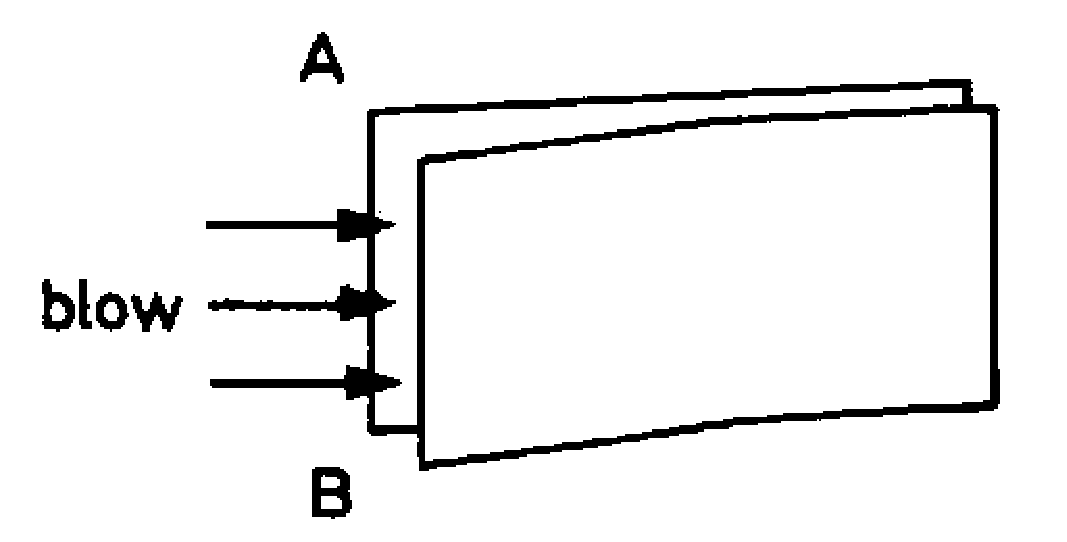
\includegraphics[width=3in]{Section34.pdf}}
\label{fig4}
\end{figure}



\chapter{Vortex Motion}
\section{The vorticity field}

The vector ${\bm{\omega}} =\nabla \times {{\bf u}}$ is twice the local angular 
velocity in the flow, and ${\bm \omega}$ is termed the 
\textbf{vorticity} of the flow (from Latin for a whirlpool).
\begin{description}
\item[(i)] Vortex lines are everywhere in the direction of the vorticity field (c.f. 
streamlines); bundles of vortex lines make up \textbf{vortex tubes}; and 
thin vortex tubes, such that their constituent vortex lines are 
approximately parallel to the tube axis are \textbf{vortex filaments} (see 
below).
\item[(ii)] The vorticity field is \textbf{solenoidal},  i.e. 
\[ \nabla . {\bm{\omega}} = 0,\]
since 
\begin{align*}
\nabla . {\bm{\omega}}
& =\nabla . \left( {\nabla \times {{\bf u}}} 
\right) \\
& =\frac{\partial }{\partial x}\left( {\frac{\partial w}{\partial 
y}-\frac{\partial v}{\partial z}} \right)+\frac{\partial }{\partial y}\left( 
{\frac{\partial u}{\partial z}-\frac{\partial w}{\partial x}} 
\right)+\frac{\partial }{\partial z}\left( {\frac{\partial v}{\partial 
x}-\frac{\partial u}{\partial y}} \right) \\
& = 0.
\end{align*}

From the divergence theorem, for any volume $V$ with boundary surface $S$,
\[
\int_S {{\bm{\omega}}. {{\bf n}}dS} =\int_V {\nabla . {\bm{\omega}} dV} 
=0,
\]
and there is zero net flux of vorticity (or vortex tubes) out of any volume: 
hence there can be no sources of vorticity in the interior of a fluid.

\begin{figure}[htbp]
\centerline{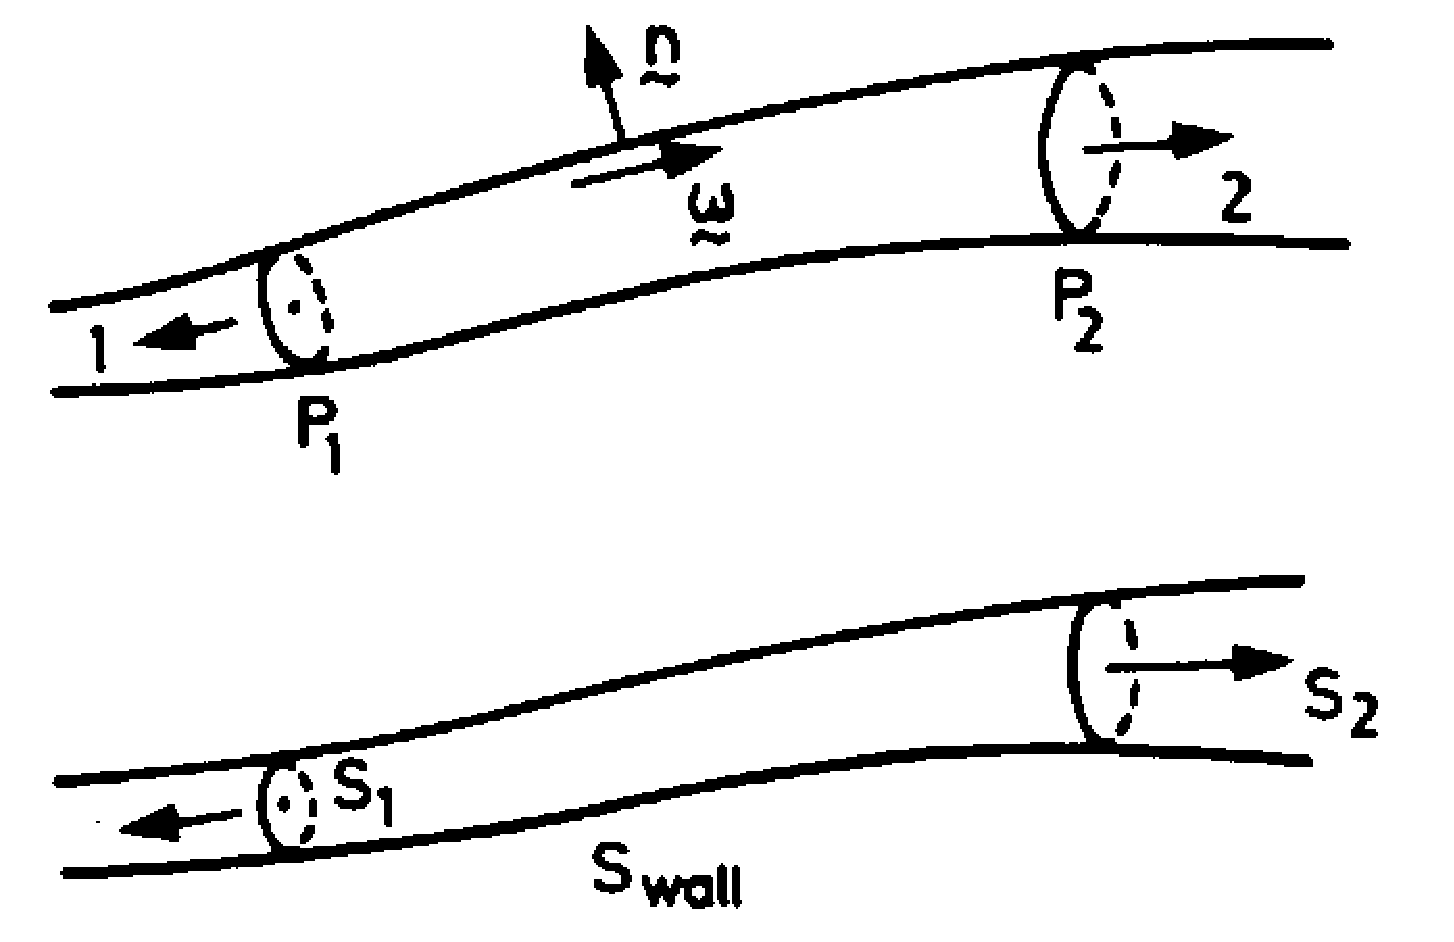
\includegraphics[width=4in]{Section42.pdf}}
\label{fig2}
\end{figure}

\item[(iii)] Consider a length $P_{1}P_{2}$ of vortex tube. From the divergence 
theorem
\[
\int_S {{\bm{\omega}}. {{\bf n}}dS} =\int_V {\nabla . {\bm{\omega}} dV} 
=0.
\]
We can divide the surface of the length $P_{1} P_{2}$ into cross-sections 
and the tube wall,
$S = S_{1} + S_{2} + S_{{wall}}$ , then
\[
\int_S {{\bm{\omega}}. {{\bf n}}dS} =\int_{S_1 } {{\bm{\omega}}. {\rm 
{\bf n}}dS} +\int_{S_2 } {{\bm{\omega}}. {{\bf n}}dS} 
+\int_{S_{wall} } {{\bm{\omega}}. {{\bf n}}dS} =0
\]
However, the contribution from the wall (where ${\bm{\omega}}\bot 
\textbf{n}$) is zero, and hence
\[
\int_{S_1 } {{\bm{\omega}}. {{\bf n}}dS} =\int_{S_2 } {{\bm{\omega}}. 
\left( {-{{\bf n}}} \right)dS} 
\]
where the positive sense for normals is that of increasing distance along 
the tube from the origin. Hence $\int_{S} {{\bm\omega}. {{\bf 
n}}dS} $ measured over a cross-section of the vortex tube with \textbf{n} 
taken in the same sense is constant, and defined as the \textbf{strength of 
the vortex tube}.

In a \textbf{thin} vortex tube, we have approximately:
\[
\int_S {{\bm{\omega}}. {{\bf n}}dS} \approx \left( {{\bm{\omega}}. {{\bf 
n}}} \right)\int_S {dS} =\omega S,
\]
and $\omega \times \hbox{area}$ = constant along the tube (a property of all 
solenoidal fields), where $\omega = | {\bm{\omega}}|$. 
\end{description}


\begin{exmp}
Show that $(\textstyle{1 \over 2}{{\bf u}}^2+p/ \rho +\Omega 
)$ is constant along a vortex line for steady, incompressible, inviscid flow 
under conservative external forces.
\end{exmp}

%\textbf{Solution}

%As before ${{\bf u}}. \nabla {{\bf u}}+\frac{1}{\rho 
%}\nabla (p+\rho \Omega )={{\bf 0}}$,

%where $\left( {{{\bf u}}. \nabla } \right){{\bf u}}=\nabla 
%\left( {\textstyle{1 \over 2}{{\bf u}}^2} \right)-{{\bf u}}\times 
%\left( {\nabla \times {{\bf u}}} \right)=\nabla \left( {\textstyle{1 
%\over 2}{{\bf u}}^2} \right)-{{\bf u}}\times w$ . (See Exercise 
%3.1.)

%Hence ${{\bf u}}\times w=\nabla \left( {\textstyle{1 \over 2}{\rm 
%{\bf u}}^2+\frac{p}{\rho }+\Omega } \right)$

%Taking \textbf{u }$.  \quad {{\bf u}}. \left( {{{\bf u}}\times 
%w} \right)=0={{\bf u}}. \nabla \left( {\textstyle{1 \over 2}{\rm 
%{\bf u}}^2+\frac{p}{\rho }+\Omega } \right)$ (4.1)

%Taking \textbf{$\omega $ }$.  \quad w. \left( {{{\bf u}}\times w} 
%\right)={{\bf 0}}=w. \nabla \left( {\textstyle{1 \over 2}{\rm 
%{\bf u}}^2+\frac{p}{\rho }+\Omega } \right)$. (4.2)

%From (4.1) $(\textstyle{1 \over 2}{{\bf u}}^2+p \mathord{\left/ 
%{\vphantom {p \rho }} \right. } \rho +\Omega 
%)$ = constant along a streamline, and from (4.2) $(\textstyle{1 \over 
%2}{{\bf u}}^2+p \mathord{\left/ {\vphantom {p \rho }} \right. 
%} \rho +\Omega )$ = constant along a vortex 
%line. Thus we have a Bernoulli equation for vortex lines as well as for 
%streamlines.

%If \textbf{$\omega $ }= \textbf{0} everywhere, then $\nabla (\textstyle{1 
%\over 2}{{\bf u}}^2+p \mathord{\left/ {\vphantom {p \rho }} \right. 
%} \rho +\Omega )={{\bf 0}}$ at every 
%point in the fluid. Consequently, $(\textstyle{1 \over 2}{{\bf 
%u}}^2+p \mathord{\left/ {\vphantom {p \rho }} \right. 
%} \rho +\Omega )$ is a constant throughout 
%the entire fluid.

\section{Circulation}
\label{subsec:circulation}

From Stokes' theorem
\[
\int_S {\left( {\nabla \times {{\bf u}}} \right)} . {{\bf 
n}}dS=\oint\limits_C {{{\bf u}}. {{\bf dx}}} ,
\]
where \textbf{n} is the unit normal to $S$, with the orientation of $C$ and the 
direction of \textbf{n} being given by the right hand rule. Hence the line 
integral of the velocity field in any circuit $C$ that passes once round a 
vortex tube is equal to the total vorticity cutting any cap $S$ on $C$, and is 
therefore equal to the strength of the vortex tube. We measure the strength 
of a vortex tube by calculating $\oint\limits_C {{{\bf u}}. {\rm 
{\bf dx}}} $ around \textbf{any circuit } $C$ enclosing the tube once only. The 
quantity 
\[ \Gamma =\oint\limits_C {{{\bf u}}. {{\bf dx}}} \]
 is termed the \textbf{circulation}. Vorticity may be regarded as 
\textbf{circulation per unit area}, and the component in any direction of 
${\bm \omega}$ is
\[
\mathop {\lim }\limits_{S\to 0} \frac{1}{S}\oint\limits_C {{{\bf 
u}}. {{\bf dx}}} 
\]
where $C$ is a loop of area $S$ perpendicular to the direction specified.

\section{The Helmholtz equation for vorticity}
\label{subsec:mylabel1}
From Euler's equation for an incompressible fluid in a conservative force 
field
\[
\frac{\partial {{\bf u}}}{\partial t}+{{\bf u}}. \nabla {\rm 
{\bf u}}=-\frac{1}{\rho }\nabla p-\nabla \Omega 
\]
or 
\[ \frac{\partial {{\bf u}}}{\partial t}+\nabla \left( {{1 
\over 2}{{\bf u}}^2} \right)-{{\bf u}}\times 
{\bm\omega} =-\frac{1}{\rho }\nabla p-\nabla \Omega ; \]
taking the curl, 
\[ \nabla \times \left( {\frac{\partial {{\bf 
u}}}{\partial t}} \right)+\nabla \times \nabla \left( {{1 \over 
2}{{\bf u}}^2} \right)-\nabla \times \left( {{{\bf u}}\times {\bm\omega}} 
\right)=-\nabla \times \nabla \left( {\frac{p}{\rho }+\Omega } 
\right). \]
But $\nabla \times \nabla \chi =0$ for all $\chi $, 
and 
\[\nabla \times \left( {{{\bf u}}\times {\bm \omega}} \right)={{\bf 
u}}\left( {\nabla . {\bm \omega}} \right)-{\bm \omega}\left( {\nabla . {{\bf u}}} 
\right)+\left( {{\bm \omega}. \nabla } \right){{\bf u}}-\left( {{{\bf 
u}}. \nabla } \right){\bm \omega}=\left( {{\bm \omega}. \nabla } \right){{\bf 
u}}-\left( {{{\bf u}}. \nabla } \right){\bm \omega} \]
as ${\bm \omega}$ is always solenoidal and \textbf{u} is solenoidal in 
an incompressible fluid. Hence we obtain
\[
\frac{D{\bm \omega}}{Dt}=\frac{\partial {\bm \omega}}{\partial t}+\left( {{{\bf u}}. 
\nabla } \right){\bm \omega}=\left( {{\bm \omega}. \nabla } \right){{\bf u}},
\]
which is the \textbf{Helmholtz vorticity equation}.

\begin{wrapfigure}{r}{3in}
\centerline{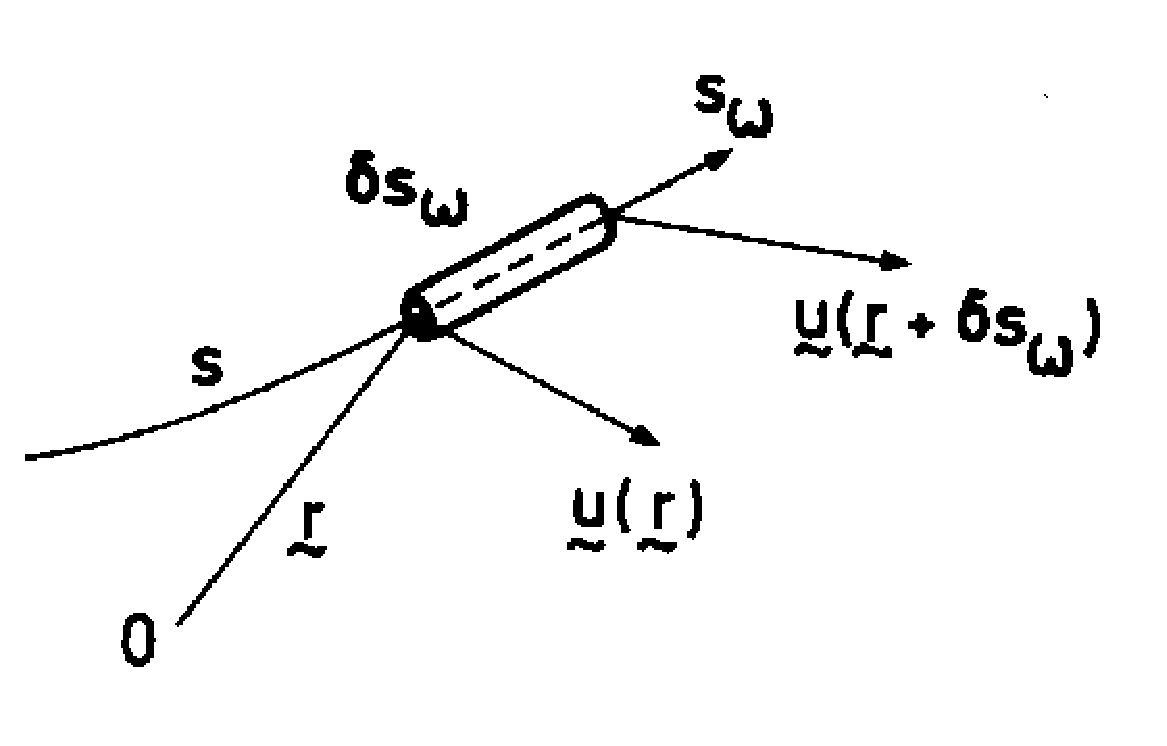
\includegraphics[width=3in]{Section43.pdf}}
\label{fig3}
\end{wrapfigure}

\subsection{Physical significance of $\left( {{\bm\omega}. \nabla } \right){\rm 
{\bf u}}$}

We can understand the significance of the term $\left( {{\bm\omega}. \nabla } 
\right){{\bf u}}$ in the Helmholtz equation by recalling that $\nabla $ 
is a directional derivative and $({\bm\omega}.  \nabla )$ is 
proportional to the derivative in the direction of ${\bm\omega}$ along 
the vortex line:
\[
\frac{D{\bm\omega}}{Dt}=\left( {{\bm\omega}. \nabla } \right){{\bf u}}=\omega \hat 
{{\bm\omega}}. \nabla {{\bf u}}=\omega \frac{\partial {{\bf u}}}{\partial 
s},
\]
where $\delta {\bf s}$ is the length of an element of vortex tube. We now resolve 
$\textbf{u}$ into components \textbf{u}$_{\omega }$ parallel to ${\bm\omega}$
 and \textbf{u}$_{\bot }$ at right angles to 
${\bm\omega}$ and hence to $\delta \textbf{s}$. Then 
\begin{align*}
 \frac{\delta s}{\omega }\frac{Dw}{Dt} &=\frac{\partial }{\partial 
s}\left( {{{\bf u}}_\omega +{{\bf u}}_\bot } \right)\delta s  \\
 & =\frac{\partial {{\bf u}}_\omega }{\partial 
s}\delta s+\frac{\partial {{\bf u}}_\bot }{\partial s}\delta s \\ 
& =\left[ {{{\bf u}}_\omega \left( {{{\bf 
x}}+d{{\bf s}}} \right)-{{\bf u}}_\omega \left( {{\bf x}} 
\right)} \right]+\left[ {{{\bf u}}_\bot \left( {{{\bf x}}+d{{\bf 
s}}} \right)-{{\bf u}}_\bot \left( {{\bf x}} \right)} \right] \\ 
\noalign{\medskip}
& \qquad \qquad \quad{\bf (A)} \qquad \qquad \qquad \qquad \qquad {\bf (B)}
 \end{align*}
\begin{description}
\item[(A)] Rate of stretching of an element: \textbf{stretching} along the
length of the filament causes relative amplification of the vorticity field;
\item[(B)] Rate of turning of an element: \textbf{turning} away from the line
of the filament causes a reduction of the vorticity in that direction, but an
increase in the new direction.
\end{description}

\section{Kelvin's Theorem}
The ideas of vorticity and circulation are important because of the 
permanence of circulation under deformation of the flow due to pressure 
forces. We next look at the rate of change of circulation round a circuit 
moving with an incompressible, inviscid fluid:
\begin{align*}
 \frac{D}{Dt}\oint {{{\bf u}}. {{\bf dx}}} & =\oint 
{\frac{D}{Dt}\left( {{{\bf u}}. {{\bf dx}}} \right)} \\ 
&  =\oint {\frac{D{{\bf u}}}{Dt}. 
{{\bf dx}}} +\oint {{{\bf u}}. \frac{D{{\bf 
dx}}}{Dt}} \\ 
 \end{align*}
 But $\oint {\frac{D{{\bf u}}}{Dt}. {{\bf dx}}} =\oint {-\nabla 
\left( {p/  {\rho +\Omega }} \right)} . {{\bf dx}}$ 
and $\oint {{{\bf u}}. \frac{D{{\bf dx}}}{Dt}} =\oint 
{{{\bf u}}. {{\bf du}}} $ (see Example below).

Hence
\begin{align*}
 \frac{D\Gamma }{Dt} & =-\oint {\nabla \left( {p/ {\rho +\Omega }} 
\right)} . {{\bf dx}}+\oint {{{\bf u}}. {{\bf du}}} \\ 
&  =\oint {d\left( {{-p}  {\rho -\Omega +\textstyle{1 \over 2}{{\bf 
u}}^{{\bf 2}}}} \right)} \\ 
 & =0 \\ 
 \end{align*}
as ${-p}/{\rho 
-\Omega +\textstyle{1 \over 2}{{\bf u}}^{{\bf 2}}}$ returns to its 
initial value after one circuit since it is a single valued function.

% \textbf{Example}

\begin{exmp}
Show using the diagram below that $\oint {{\rm 
{\bf u}}. \frac{D{{\bf dx}}}{Dt}} =\oint {{{\bf u}}. 
{{\bf du}}} $.
\end{exmp}

\begin{figure}
\centerline{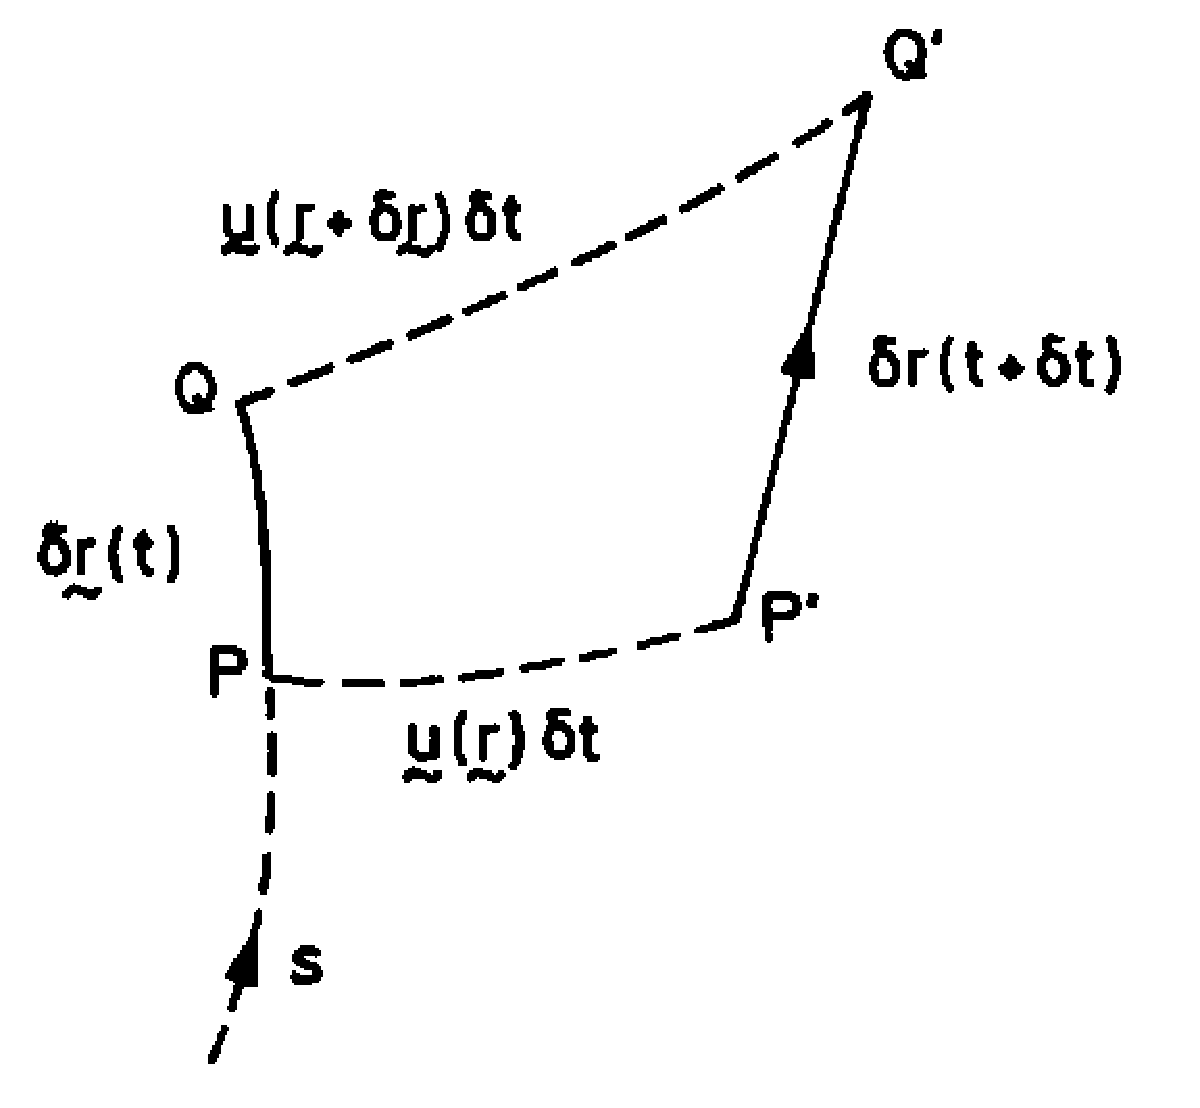
\includegraphics[width=2.5in]{Section44.pdf}}
\label{fig4}
\end{figure}



%\textbf{Solution}

%Suppose that the elementary vector $\overline {PQ} =\delta {{\bf x}}$ at 
%t is advected with the flow to$\overline {{P}'{Q}'} =\delta {{\bf 
%x}}\left( {t+\delta t} \right)$. Then

%\textbf{$\delta $}$\delta {{\bf x}}\left( {t+\delta t} \right)\approx 
%-{{\bf u}}\left( {{\bf x}} \right)\delta t+\delta {{\bf 
%x}}\left( t \right)+{{\bf u}}\left( {{{\bf x}}+\delta {{\bf x}}} 
%\right)\delta t$

%or $\delta {{\bf x}}\left( {t+\delta t} \right)-\delta {{\bf 
%x}}\left( t \right)\approx \left[ {{{\bf u}}\left( {{{\bf x}}+\delta 
%{{\bf x}}} \right)-{{\bf u}}\left( {{\bf x}} \right)} 
%\right]\delta t$.

%Hence $\mathop {\lim }\limits_{\delta t\to 0} \frac{\delta {{\bf 
%x}}\left( {t+\delta t} \right)-\delta {{\bf x}}\left( t \right)}{\delta 
%t}=\mathop {\lim }\limits_{\delta s\to 0} \frac{{{\bf u}}\left( {{\rm 
%{\bf x}}+\delta {{\bf x}}} \right)-{{\bf u}}\left( {{\bf x}} 
%\right)}{\delta s}\delta s$,

%from which it follows that $\frac{D}{Dt}\delta {{\bf x}}\approx 
%\frac{\partial {{\bf u}}}{\partial s}\delta s\approx \delta {{\bf 
%u}}$ in a fixed reference frame 0xyz, where $\left| {\delta {{\bf x}}} 
%\right|=\delta s$ and s is arc length along the path PQ. In the limit as 
%$\delta {{\bf x}}\to d{{\bf x}}$, $\delta {{\bf u}}\to d{\rm 
%{\bf u}}$, and $\frac{D}{Dt}d{{\bf x}}=d{{\bf u}}$ .

\subsection{Helmholtz theorem: vortex lines move with the fluid}

\begin{wrapfigure}{r}{2.in}
\centerline{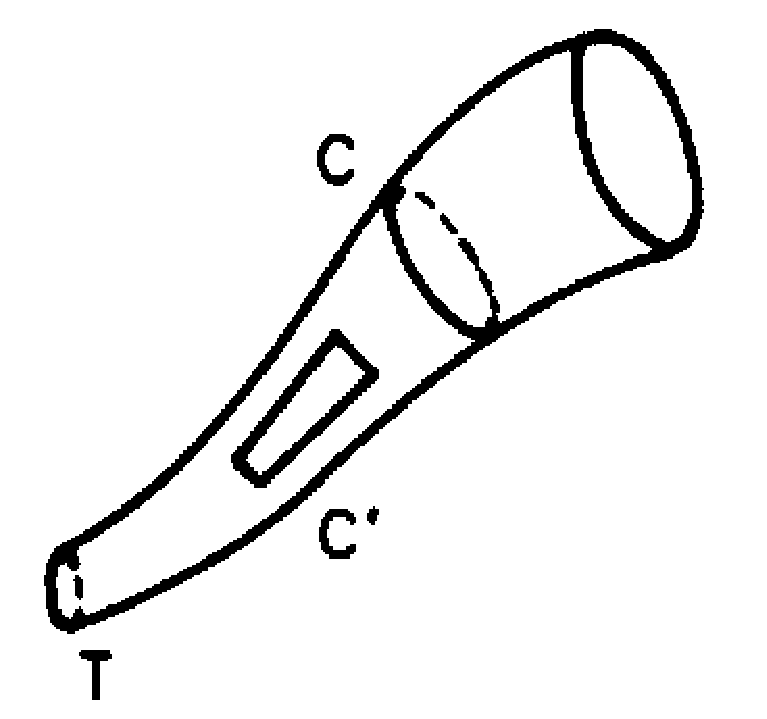
\includegraphics[width=2.in]{Section45.pdf}}
\label{fig5}
\end{wrapfigure}

Consider a tube of particles $T$, which at the instant $t$ forms a vortex tube 
of strength $\kappa $. At that time the circulation round any circuit $C'$ 
lying in the tube wall, but \textit{not} linking (i.e. embracing) the tube is zero, 
while that in an circuit $C$ linking the tube \textit{once} is $\kappa $. These 
circulations suffer no change moving with the fluid: hence the circulation 
in $C'$ remains zero and that in $C$ remains $\kappa $, i.e. the fluid 
comprising the vortex tube at $T$ continues to comprise a vortex tube (as the 
vorticity component normal to the tube wall --- measured in $C'$ --- is always 
zero), \textit{and} the strength of the vortex remains constant. A vortex line is the 
limiting case of a small vortex tube: hence vortex lines move with (are 
frozen into) inviscid fluids.

\subsection{A flow which is initially irrotational remains irrotational}

Circulation is advected with the fluid in inviscid flows, and vorticity is 
``circulation per unit area". If initially $\Gamma = 0$ for all closed 
circuits in some region of flow, it must remain so for all subsequent times. 
Motion started from rest is initially irrotational (free from vorticity) and 
will therefore remain irrotational provided that it is inviscid.

\begin{center}
\textbf{The direction of the vorticity turns as the vortex line turns, and 
its magnitude increases as the vortex line is stretched.}
\end{center}

The circulation round a thin vortex tube remains the same; as it stretches 
the area of section decreases and
\begin{center}
\textbf{Circulation / Area = Vorticity}
\end{center}
increases in proportion to the stretch.

\section{Rotational and irrotational flow}

\begin{wrapfigure}{r}{2.5in}
\centerline{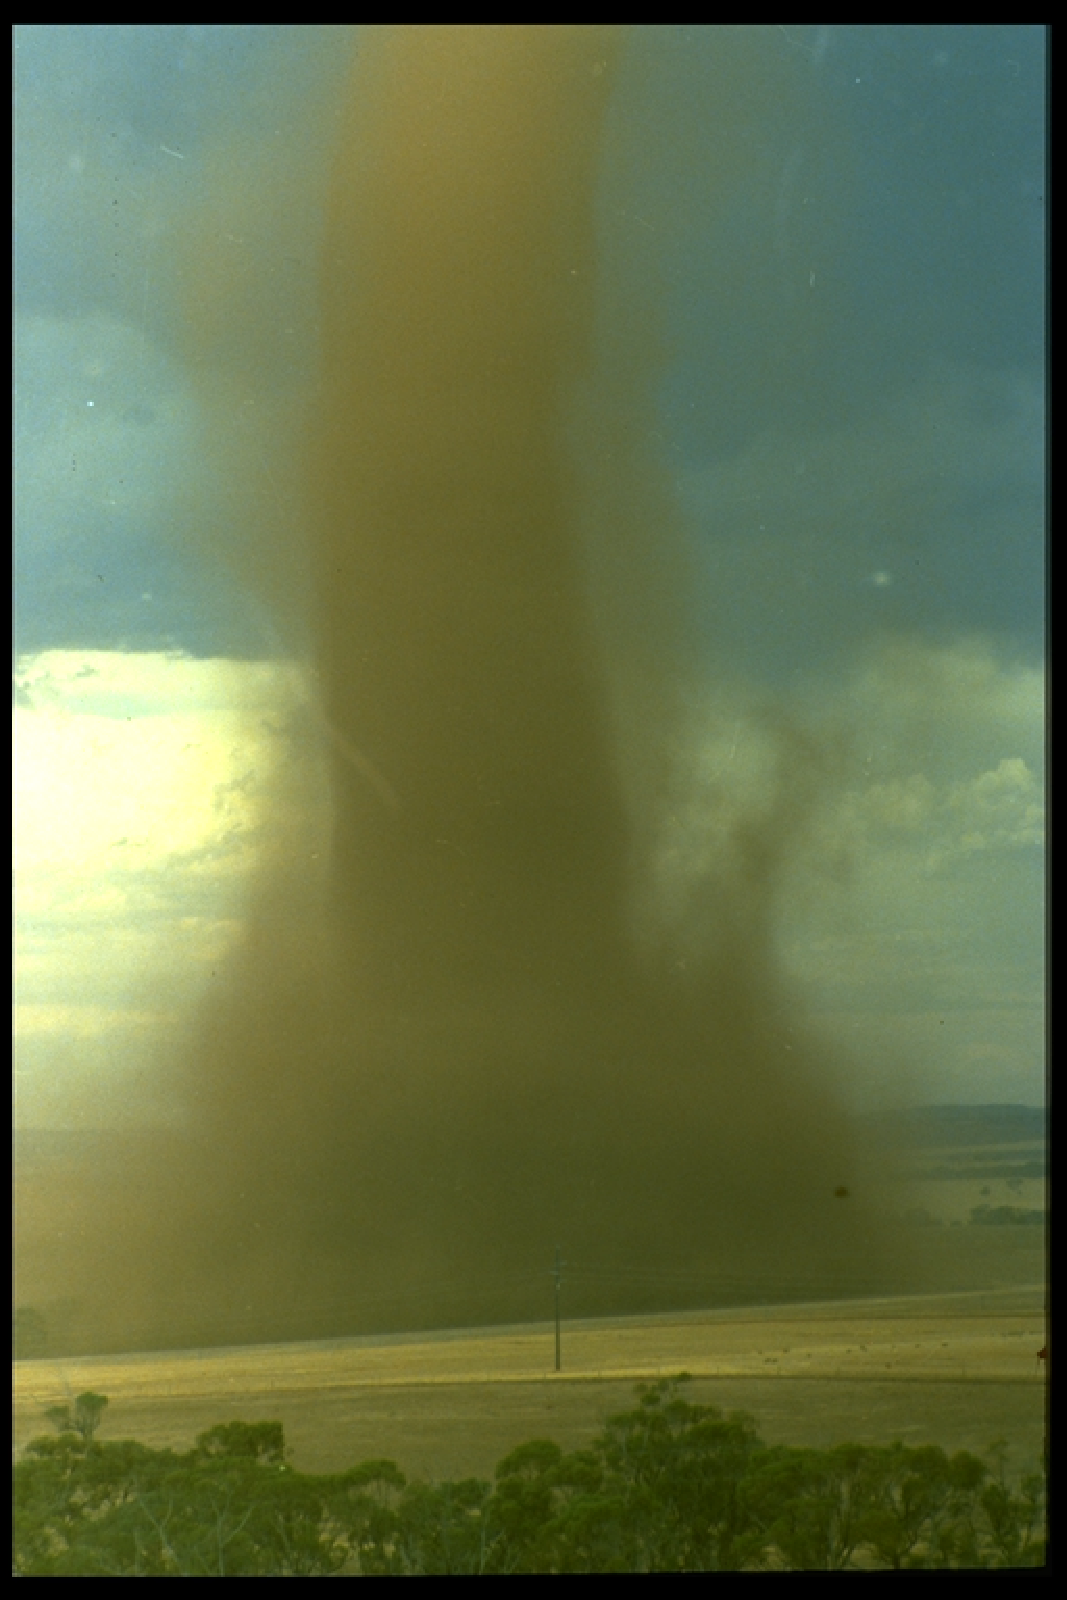
\includegraphics[width=2.5in]{Section46.pdf}}
\label{fig6}
\end{wrapfigure}

Flow in which the vorticity is everywhere zero ${\bm\omega} =\nabla \times {{\bf 
u}}$ is called \textbf{irrotational}. Other terms in use are \textbf{vortex 
free, ideal, and perfect}. Much of fluid dynamics used to be concerned with 
analysing irrotational flows and deciding where these give a good 
representation of real flows, and where they are quite wrong.

\begin{exmp}
Consider a small circular element of fluid in solid body rotation with angular velocity $\Omega$. Using 
cylindrical polar coordinates, show that the circulation around the circular element 
is
\[ \Gamma = 2\Omega \pi r^2, \]
and that the vorticity is
\[ \bm\omega = 2\Omega{\bf k}. \]
\end{exmp}

%Consider a small circular element of fluid in solid body rotation. Using 
%cylindrical polar coordinates, the circulation around the circular element 
%is
%\[ \Gamma =\oint {{{\bf u}}. d{{\bf x}}} =\int_0^{2\pi } 
%{v\left( {rd\theta } \right)=} \Omega r^2\int_0^{2\pi } {d\theta 
%=} 2\Omega \pi r^2
%\Gamma =\oint_ {u. dr=} \int_0^{2\pi } {vrd\theta } =\Omega r^2\int_0^{2\pi } 
%{d\theta =2\Omega } \pi r^2$ Since the area of the element is $\pi $r$^{2}$, the vorticity is 2$\Omega $, which is twice the angular velocity.

% \textbf{Example}
\begin{exmp}
Consider the shear flow \textbf{u} = ($\Lambda $z,0,0). Show that although the 
streamlines are straight and parallel to the $x$-axis, the flow is not 
irrotational.
\end{exmp}

%Consider the shear flow \textbf{u} = ($\Lambda $z,0,0). Although the 
%streamlines are straight and parallel to the x-axis, the flow is not 
%irrotational since $\nabla \times {{\bf u}}=\left( {0,\Lambda ,0} 
%\right)$.

We have neglected \textbf{compressibility} and \textbf{viscosity}. It can be 
shown that the neglect of compressibility is not very serious even at 
moderately high speeds, but the effect of neglecting viscosity can be 
disastrous. Viscosity \textbf{diffuses} the vorticity (much as conductivity 
diffuses heat) and progressively blurs the results derived above, the errors 
increasing with time.

There is no term in the Helmholtz equation ${D{\bm\omega}}/{Dt}=\left( {{\bm\omega}. \nabla 
} \right){{\bf u}}$ corresponding to the generation of vorticity (the 
term ${\bm\omega}. \nabla {{\bf u}}$ represents processing by stretching and 
turning of vorticity already present). It follows, therefore, that in 
homogeneous fluids all \textbf{vorticity must be generated at boundaries 
}(more on this later). In real (viscous) fluids, this vorticity is carried 
away from the boundary by diffusion and is then advected into the body of 
the flow. But in inviscid flow vorticity cannot leave the surface by 
diffusion, nor can it leave by advection with the fluid as no fluid 
particles can leave the surface. It is this inability of inviscid flows to 
model the diffusion/advection of vorticity generated at boundaries out into 
the body of the flow that causes most of the failures of the model.

In inviscid flows we are left with a free slip velocity at the boundaries, 
which we may interpret as a thin vortex sheet wrapped around the boundary.

\section{Vortex sheets}
Consider a thin layer of thickness $\delta $ in which the vorticity is large 
and is directed along the layer (parallel to $0y$), as sketched. The vorticity 
is
\[
\eta =\frac{\partial u}{\partial z}-\frac{\partial w}{\partial x}\quad ,
\]
where $\partial u/\partial z$ is large (but not $\partial w/\partial x$, 
which would lead to very large $w$).

\begin{wrapfigure}{r}{2.5in}
\centerline{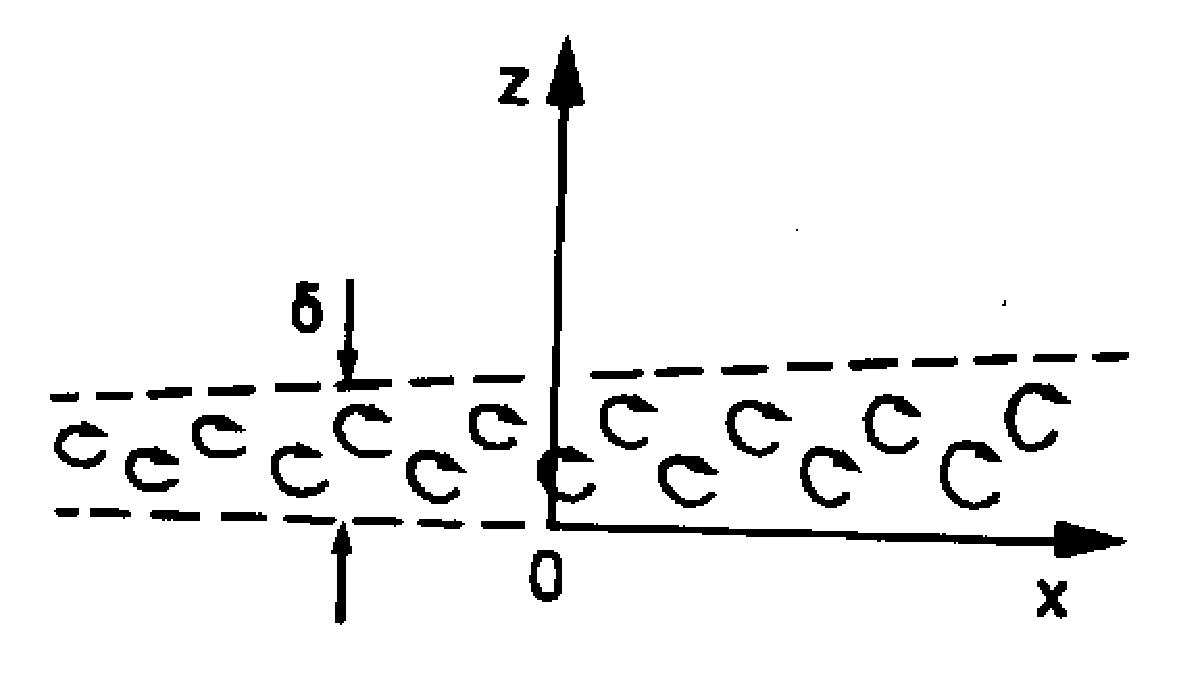
\includegraphics[width=2.5in]{Section47.pdf}}
\label{fig7}
\end{wrapfigure}

We can suppose that within the vortex layer $u = u_{0}+\omega z$ changing 
from $u_{0}$ to $u_{0}+\omega \delta $ between $ z = 0$ and $\delta $, 
with mean vorticity
\[
\frac{\left( {u_0 +\omega \delta } \right)-u_0 }{\delta }=\omega 
\]
This vortex layer provides a sort of roller action, though it is not of 
course rigid, and it also suffers high rate-of-strain.

If we idealize this vortex layer by taking the limit $\delta \to  0$, 
$\omega  \to \infty $, with $\omega \delta $ remaining finite, we 
obtain a \textbf{vortex sheet}, which is manifest only through the free slip 
velocity. Such vortex sheets follow the contours of the boundary and clearly 
may be curved. They are infinitely thin sheets of vorticity with infinite 
magnitude across which there is finite difference in tangential velocity, 
$\omega \delta $.

\section{Line vortices}
We can represent approximately also strong thin vortex tubes (e.g. 
tornadoes, waterspouts, draining vortices) by \textbf{vortex lines} without 
thickness. The circulation in a circuit round the tube tends to a definite 
non-zero limit as the circuit area $S \to 0$. If the flow outside the 
vortex is irrotational then all circuits round the vortex have the same 
circulation (by Stokes' theorem), the strength $\kappa $ of the vortex being
\[\oint {{{\bf u}}. {{\bf dx}}} \to \kappa \quad\hbox{as}\quad C \to  0 . \]
As the flow outside the vortex is irrotational, the circulation is zero 
around any circuit that does not enclose the vortex.

\begin{exmp}
Consider an isolated line vortex aligned with the $z$-axis. Show that a
radially symmetric solution is
\[ u=0, \quad v = \frac{\kappa }{2\pi r}, \]
where $\kappa$ is the circulation around a circuit enclosing the $z$-axis. 
\end{exmp}

%\textbf{Example }

%Consider an isolated line vortex aligned with the z-axis. In cylindrical 
%polar coordinates the vorticity is
%\[
%w=\nabla \times {{\bf u}}=\left( {0,0,\frac{1}{r}\left( {\frac{\partial 
%\left( {rv} \right)}{\partial r}-\frac{\partial u}{\partial \theta }} 
%\right)} \right)={{\bf 0}}
%\]
%if the flow is irrotational (except on r = 0). If follows that, ${\partial 
%\left( {rv} \right)} \mathord{\left/ {\vphantom {{\partial \left( {rv} 
%\right)} {\partial r}}} \right. } {\partial 
%r}={\partial u} \mathord{\left/ {\vphantom {{\partial u} {\partial \theta 
%}}} \right. } {\partial \theta }$, and hence,
%\[
%\frac{d\Gamma }{dr}=\frac{d}{dr}\int_0^{2\pi } {v\left( {rd\theta 
%} \right)} =\int_0^{2\pi } {\frac{\partial \left( {rv} 
%\right)}{\partial r}d\theta =} \int_0^{2\pi } {\frac{\partial 
%u}{\partial \theta }d\theta =} 0.
%\]
%As expected, the circulation in circular circuits around the z-axis is 
%constant and independent of the radius of the circuit. Take this circulation 
%to be $\kappa $. Then,
%\[
%\int_0^{2\pi } {rvd\theta } =\kappa .
%\]
%or $\int_0^{2\pi } {vd\theta } =\frac{\kappa }{r}$.

%Seeking a solution with radial symmetry, v is independent of $\theta $ and 
%\[
%v\int_0^{2\pi } {d\theta } =2\pi v=\frac{\kappa }{r},
%\]
%or $v=\frac{\kappa }{2\pi r}$.

%As the line vortex is approached, the tangential velocity $\to  \quad \infty $ 
%like (distance)$^{-1}$. Note particularly that the line vortex flow field is 
%one in which every element of fluid is ``rotating'' in a circular path about 
%the vortex but that the vorticity distribution is zero at all points of the 
%flow for which r $\ne $ 0. There is just one velocity distribution that 
%makes this possible -- that for which the velocity is entirely tangential 
%and decays as (distance)$^{-1}$.

The effect of viscosity is to thicken vortex sheets and line vortices by 
diffusion; however, the effect of diffusion is often slow relative to that 
of advection by the flow, and as a result large regions of flow will often 
remain free from vorticity. Vortex sheets at surfaces diffuse to form 
\textbf{boundary layers} in contact with the surfaces; or if free they often 
break up into line vortices. Boundary layers on bluff bodies often 
\textit{separate} or break away from the body, forming a \textbf{wake} of rotational, 
retarded flow behind the body, and it is these wakes that are associated 
with the \textbf{drag} on the body. (More on separation later.)

\section{Motion started from rest impulsively}
Viscosity (which is really just distributed internal fluid friction) is 
responsible for retarding or damping forces which cannot begin to act until 
the motion has started; i.e. \textbf{take time to act}. Hence any flow will 
be \textbf{initially} irrotational everywhere except at actual boundaries. 
Within increasing time, vorticity will be diffused from boundaries and 
advected and diffused out into the flow.

Motion started from rest by an \textbf{instantaneous impulse} must be 
irrotational. If we integrate the Euler equation over the time interval $(0, 
\delta t)$:
\[
\int_0^{\delta t} {\frac{D{{\bf u}}}{Dt}} 
dt=\int_0^{\delta t} {{\bf F}} dt-\int_0^{\delta t} 
{\frac{\nabla p}{\rho }} dt
\]
or 
\[\left[ {{\bf u}} \right]_0^\delta =\int_0^{\delta t} {\rm 
{\bf F}} dt-\frac{1}{\rho }\nabla \int_0^{\delta t} p dt. \]

In the limit $\delta t \to  0$ for start-up by an instantaneous impulse, 
the impulse of the body force $\to  0$ (as the body force is unaffected by 
the impulsive nature of the start) and
\[
{{\bf u}}-{{\bf u}}_{{0}} =-\frac{1}{\rho }\nabla P,
\]
where the fluid responds instantaneously with the impulsive pressure field 
$P=\int_0^{\delta t} {pdt} $, and the impulse on a fluid element is 
$-\nabla P$ per unit volume, producing a velocity from rest of 
\[
{{\bf u}}=-\frac{1}{\rho }\nabla P.
\]
This is irrotational as $\nabla \times {{\bf u}}=-\frac{1}{\rho }\nabla 
\times \nabla P={{0}}$.

\section{Generation of circulation at boundaries}

Consider now how circulation (or vorticity) is generated. An infinite plate 
moves to the right with speed $U$. Consider the circulation around a small 
circuit $ABCD$ centred about the point $O$ on the surface of the plate, where 
${\overline {BC} } / {\overline {AB} }\ll 1$. The 
circulation is
\begin{align*}
 \int_{ABCDA} {{{\bf u}}. {{\bf dx}}} 
 & =\int_{{A}'A} {w\ dz+} \int_{AB} {\left( {u-U} \right)dx+} 
\int_{B{B}'} {wdz} \\ 
 & =\int_{{-\delta x} / 2}^{{\delta x}/ 2} {\left( {u-U} 
\right)dx} \\ 
 & =\left( {u-U} \right)\delta x \\ 
 \end{align*}

\begin{wrapfigure}{r}{3in}
\centerline{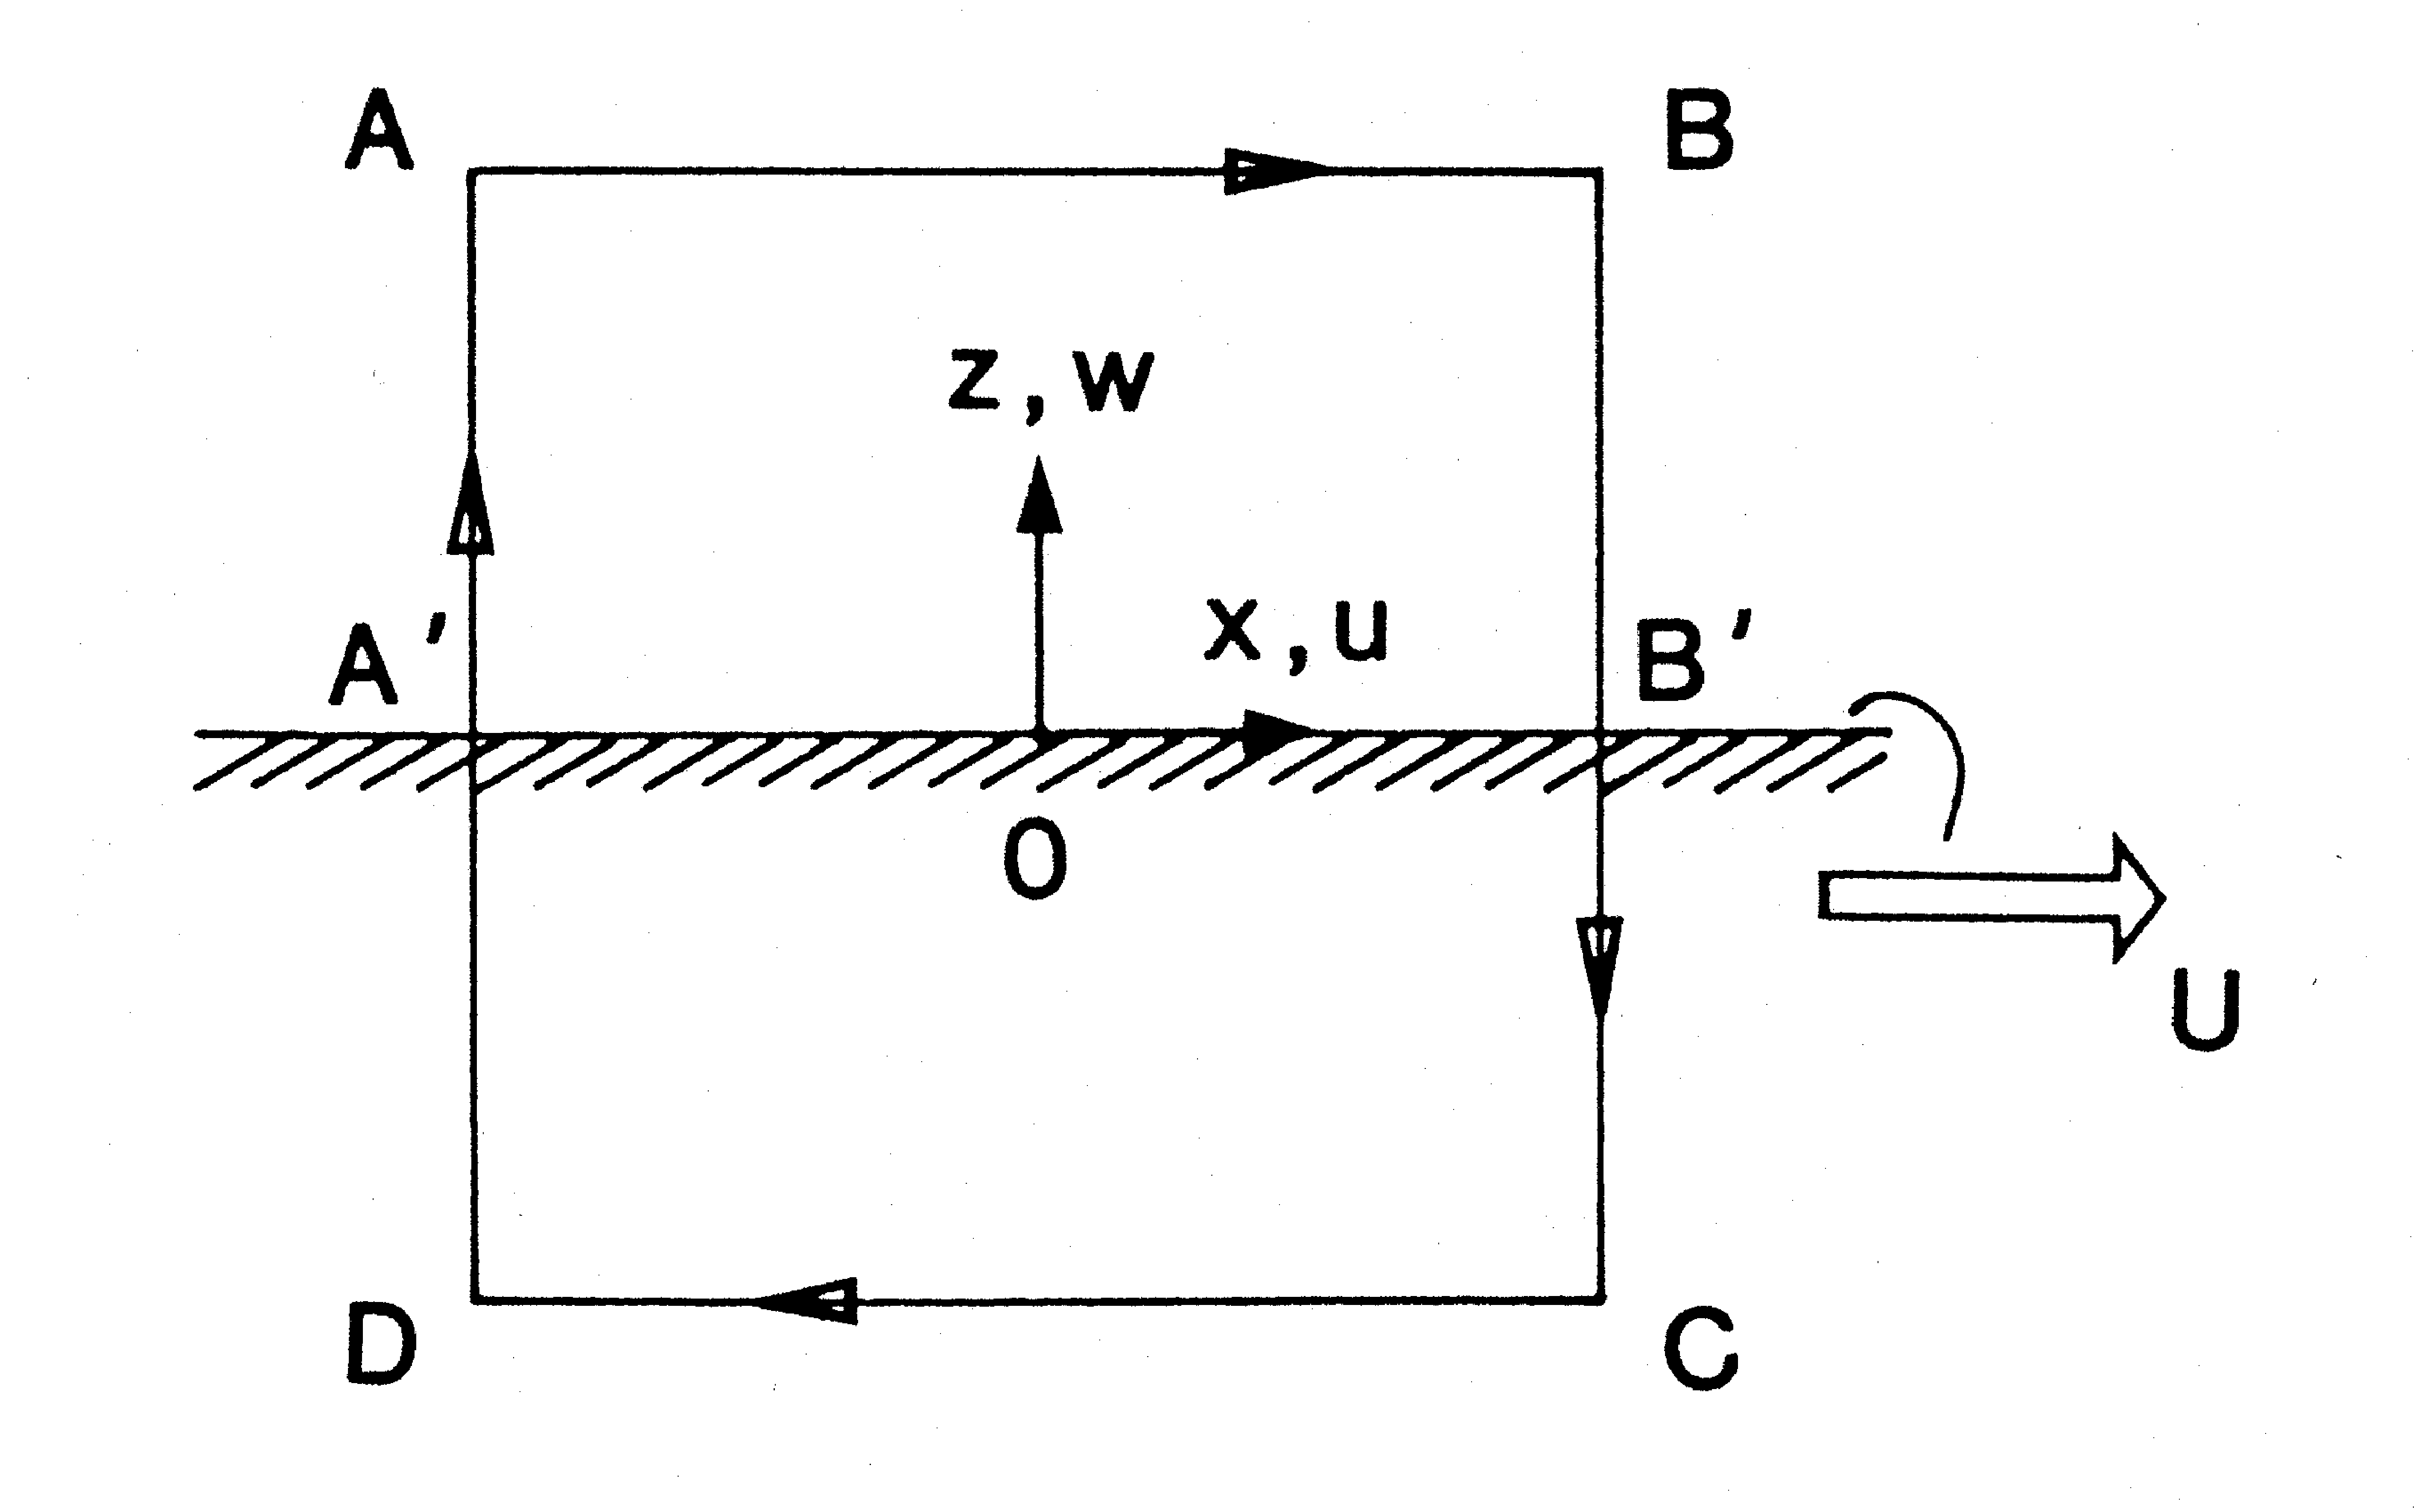
\includegraphics[width=3in]{Section48.pdf}}
\label{fig8}
\end{wrapfigure}

Hence, the circulation \textbf{per unit length} (in the $x$ direction) is $L = 
\left( {u-U} \right)$. Had the boundary been positioned on top of the fluid 
instead of below, we would have found the circulation per unit length to be 
$-\left( {u-U} \right)$. 

Taking the material derivative of this expression and using the $x$-component 
of the Navier-Stokes equation gives, 
\[
\frac{DL}{Dt}=-\frac{1}{\rho }\frac{\partial p}{\partial x}+\nu \nabla 
^2u-\frac{dU}{dt},
\]
at the lower boundary. We see that the generation of circulation per unit 
length (and hence vorticity) at a boundary is due solely to the tangential 
pressure gradient and the acceleration of the boundary. The viscous 
diffusion simply redistributes the vorticity.

\subsection*{Exercises}
\begin{enumerate}
\item Consider the shear flow $\textbf{u} = (\Lambda z, 0, 0)$. Choose any 
rectangular contour and calculate the circulation. Show that the circulation 
per unit area is $\Lambda $.

\item Assume that a tornado can be approximated as a line vortex in which the 
velocity decays as (distance)$^{-1}$. Suppose that the tangential wind is 20 
ms$^{-1}$ at a radius of 2 km. What is the circulation? What is the wind 
speed at a radius of 500 m?

\item Does fluid with velocity
\[
{{\bf u}}=\left[ {z-\frac{2x}{r},2y-3z-\frac{2y}{r},x-3y-\frac{2z}{r}} 
\right]
\]
possess vorticity, where $\textbf{u} = (u,v,w)$ is the velocity in the 
Cartesian frame, $\textbf{r} = (x,y,z)$ and $r^{2} = x^{2} +y^{2} + 
z^{2}$? What is the circulation in the circle $x^{2} + y^{2} = 9, z = 0$? 
Is this flow incompressible?

\item Given the velocity field is $\textbf{u} = (xy, 0, 0)$,  calculate the vorticity,
calculate the circulation around the rectangular circuit $(1,1,0)$, $(-1,1,0)$, 
$(-1,-1,0)$, $(1,-1,0)$. Is the flow irrotational? Why?
\end{enumerate}

\cleardoublepage

\chapter{One Dimensional Viscous Flows}
A viscous flow is one in which the fluid immediately above some level exerts 
a stress on the fluid below it and visa versa. An inviscid fluid 
is one in which this stress has no tangential component.

Newtonian fluids are those for which the shear stress $\tau $ is 
proportional to the velocity gradient, i.e.,
\[
\tau =\mu \frac{du}{dz},
\]
where $\mu $ is the coefficient of viscosity. The kinematic viscosity is 
$\nu =\mu /\rho $.

Roughly speaking, viscosity is more important close to the boundary than in 
the overlying fluid because it is close to the boundary that the velocity 
gradients are largest. In general the velocity gradients are largest near 
the boundary because the fluid must satisfy a no slip boundary condition. 

We examine now a class of viscous flow for which exact solutions can be 
found.

\section{One-dimensional flows}
The central difficulty of solving the Navier-Stokes equations lies in the 
non-linear term ${{\bf u}}. \nabla {{\bf u}}$. However, in 
one-dimensional flows only a single component of velocity is non-zero, say 
${{\bf u}}=\left( {0,0,w} \right)$. Then from the continuity equation, 
\[
\frac{\partial u}{\partial x}+\frac{\partial v}{\partial 
y}+\frac{\partial w}{\partial z}=0,
\]
whence $w$ is independent of $z$. It follows that
\begin{align*}
 {{\bf u}}. \nabla {{\bf u}}& =\left( 
{u\frac{\partial }{\partial x}+v\frac{\partial }{\partial 
y}+w\frac{\partial }{\partial z}} \right)(u,v,w) \\ 
&  =\left( {0,0,w\frac{\partial w}{\partial 
z}} \right) \\ 
& ={{\bf 0}} \\ 
 \end{align*}
and in this case many of the problems of solution disappear.

\section{Steady plane Couette flow}
Consider a steady $(\partial /\partial t = 0)$ viscous flow confined 
between two rigid plates, one at $z = 0$ and the other at $z = h$. Let the lower 
boundary $z = 0$ be fixed; while driving the upper boundary $z = h$ in its own 
plane with velocity $(U,0,0)$. Suppose that the flow independent of the $y$ 
coordinate ($\partial /\partial y = 0$ and $v = 0$). Assume that all 
$x$-positions are identical so that there can be no change in the $x$-direction 
($\partial /\partial x = 0$). The solution to this problem is called 
\textit{Couette} flow and is one of the classical problems in fluid dynamics.

From continuity 
\[\frac{\partial u}{\partial x}+\frac{\partial 
v}{\partial y}+\frac{\partial w}{\partial z}=0, \]
giving 
\[\frac{\partial w}{\partial z}=0.\]
Hence $w$ is independent of $z$ as well as $x$, $y$ and $t$. Since $w = 0$ on the bottom 
boundary, it must vanish everywhere. Consequently ${{\bf u}}=\left[ 
{u\left( z \right),0,0} \right]$.

The Navier-Stokes equations reduce to
\[
0=-\frac{1}{\rho }\frac{\partial p}{\partial x}+\nu 
\frac{d^2u}{dz^2},\quad 0=-\frac{1}{\rho }\frac{\partial 
p}{\partial y},\quad 0=-\frac{1}{\rho }\frac{\partial 
p}{\partial z},
\]
where $p$, the dynamic pressure, is independent of $x$, $y$ and $z$ (although there 
is, of course, a hydrostatic pressure satisfying ${\partial p} /{\partial z}=-\rho g$. It follows that 
\[
\frac{d^2u}{dz^2}=0,
\]
from which $u=Az+B$.

But at $z=0,u=0\Rightarrow 
B=0$ and at $z=h,u=U\Rightarrow 
A=U/h$.
Hence 
\[ u=U\frac{z}{h}. \]

The velocity profile is linear and the vorticity is therefore constant 
throughout the fluid. The vorticity is generated as the upper boundary is 
set in motion and subsequently diffuses across the channel. 

The shearing stress is $\tau =\mu \left( {{du} /{dz}} 
\right)=\mu U / h$. This result implies that in steady motion 
the tangential stress exerted \textit{by} the upper plate is transmitted across the 
channel without change in value to the lower plate (c.f. fluid transmission).

\section{Steady plane Poseuille flow}
Steady plane Poiseuille flow is driven between parallel fixed walls by an 
applied pressure gradient, and was studied initially in connection with 
blood flow. At the boundaries $\textbf{u} = \textbf{0}$ at $z = 0$ and $z = h$. As 
in Couette flow the velocity field is assumed to be independent of $x$ and $y$, 
which from continuity and the lower boundary condition implies that $w = 0$. 
Consequently, ${{\bf u}}=\left[ {u\left( z \right),0,0} \right]$. 
However, if the flow is driven left to right there must be a corresponding 
drop in (dynamic) pressure (i.e. $\partial p/\partial x <0$).

The Navier-Stokes equations reduce exactly as for Couette flow to
\[
0=-\frac{1}{\rho }\frac{\partial p}{\partial x}+\nu 
\frac{d^2u}{dz^2},\quad 0=-\frac{1}{\rho }\frac{\partial 
p}{\partial y},\quad 0=-\frac{1}{\rho }\frac{\partial 
p}{\partial z}
\]
Thus, $p$ is independent of $t$, $y$ and $z$ so that $p = p(x)$, whence
\[
\frac{d^2u}{dz^2}=\frac{1}{\rho \nu }\frac{dp}{dx}.
\]
But ${d^2u} / {dz^2}$ is a function of $z$ only, and ${dp} / {dx}$ a function
of $x$ only. Consequently, the only possibility is that both
are equal to a constant, $-\gamma $ (say). Thus 
\[
\frac{d^2u}{dz^2}=-\frac{\gamma }{\mu },
\]
from which 
\[ u=-\frac{\gamma }{2\mu }z^2+Az+B, \]
where 
\[ 0=-\frac{\gamma }{2\mu }. 0+A. 
0+B \quad \Rightarrow \quad B=0, \]
and 
\[ 0=-\frac{\gamma }{2\mu 
}h^2+Ah \quad \Rightarrow \quad A=\frac{\gamma h}{2\mu }. \]
Therefore, 
\[ u=\frac{\gamma }{2\mu }z(h-z), \]
which defines a quadratic profile.

The shearing stress $\tau ={\gamma (h-2z)} / 2$ 
is zero at the centre plane of the channel and takes its maximum values at 
the wall. In this case shearing stress is transmitted out to both walls, 
acting forwards along each (in this sign convention), and 
serving to transmit the pressure gradient force out to the walls, 
allowing steady flow (without acceleration).

The vorticity is $\eta ={\gamma (h-2z)}  / {\left( {2\mu } \right)}$. Physically, positive 
(negative) vorticity is continuously generated at the lower (upper) boundary 
and diffuses upward (downward). These positive and negative vorticities 
mutually annihilate at $z = 0$. 

\subsection*{Exercises}
\begin{enumerate}
\item Mixed Couette--Poiseuille flow is driven in a layer of uniform 
incompressible fluid between two parallel plates at $z = 0$ and $z = h$ by 
moving the upper plate steadily in its own plane in the $x$-direction with 
velocity $U$ and applying an \textit{opposing} pressure gradient ${dp} /  {dx}=\gamma >0$. 
Find the velocity profile in the flow and the volume flux. Find also the 
pressure gradient required to produce zero net volume flux per unit $y$-width.

\item Consider the time dependent Couette problem. A viscous fluid at rest is 
confined between two rigid plates, one at $z = 0$ and the other at $z = h$. The 
lower boundary is fixed, but at $t = 0$ the upper boundary is impulsively set 
in motion in its own plane with velocity $(U,0,0)$. Calculate the velocity and 
vorticity profiles as a function of time. 

\item Find the velocity field for a steady viscous flow through an
axisymmetric pipe of radius $a$ under a constant applied pressure gradient
(i.e. Poiseuille flow in cyclindrical polar coordinates).

\item Show that in the (slab symmetric) version of the Poiseuille flow problem, 
negative vorticity is being continuously generated at the upper boundary 

\item An incompressible fluid occupies the space $0<z<\infty $ above a plane 
rigid boundary $z = 0$, which oscillates in the $x$-direction with 
velocity $U\cos \left( {\alpha t} \right)$. (Unlike a Poiseuille flow, there 
is no applied pressure gradient.) Show the velocity field has the form ${\rm 
{\bf u}}=\left[ {u\left( {z,t} \right),0,0} \right]$ and satisfies 
\[ \frac{\partial u}{\partial t}=\nu \frac{\partial ^2u}{\partial z^2}. \]
 Seek 
a solution of the form $u=Re\left\{ {f\left( z \right)e^{i\alpha t}} 
\right\}$, where $Re\left\{ \bullet \right\}$ means ``the real part of''. 
Show that 
\[ u(z,t)=Ue^{-kz}\cos \left( {kz-\alpha t} \right), \]
 where $k=\sqrt 
{\alpha / {2\nu }} $.

\end{enumerate}

\cleardoublepage


\chapter{Boundary Layers in Nonrotating Fluids}
The Navier-Stokes' equation is the statement of Newton's second law of 
motion for a viscous fluid. It reads
\begin{equation}
\label{eq1}
\frac{D{{\bf u}}}{Dt}=-\frac{1}{\rho }\nabla p+\nu \nabla ^2{{\bf 
u}}.
\end{equation}
The quantity $\nu $ is called the \textbf{kinematic viscosity}. For air, 
$\nu $ = 1.5 $\times $ 10$^{-5}$ m$^{2}$s$^{-1}$; for water $\nu $ = 1.0 
$\times $ 10$^{-6}$ m$^{2}$s$^{-1}$.

The relative importance of viscous effects is characterized by the Reynolds 
number $Re$, a nondimensional number defined by
\[
Re=\frac{UL}{\nu },
\]
where $U$ and $L$ are typical velocity and length scales respectively. The 
Reynold's number is a measure of the ratio of the acceleration term to the 
viscous term in (\ref{eq1}). For example, the diameter of a cricket ball 
is about 75 mm. If the balled is bowled at 100 km hr$^{-1}$ (= 28 
ms$^{-1})$, the Reynolds number is 1.4 $\times $ 10$^{5}$. 

For many flows of interest, $Re \gg 1$ and viscous effects are relatively 
unimportant. However, these effects are \textbf{always} important near 
boundaries, even if only in a thin ``boundary-layer" adjacent to the 
boundary.

\section{Flow over a flat plate}
\begin{figure}[htbp]
\centerline{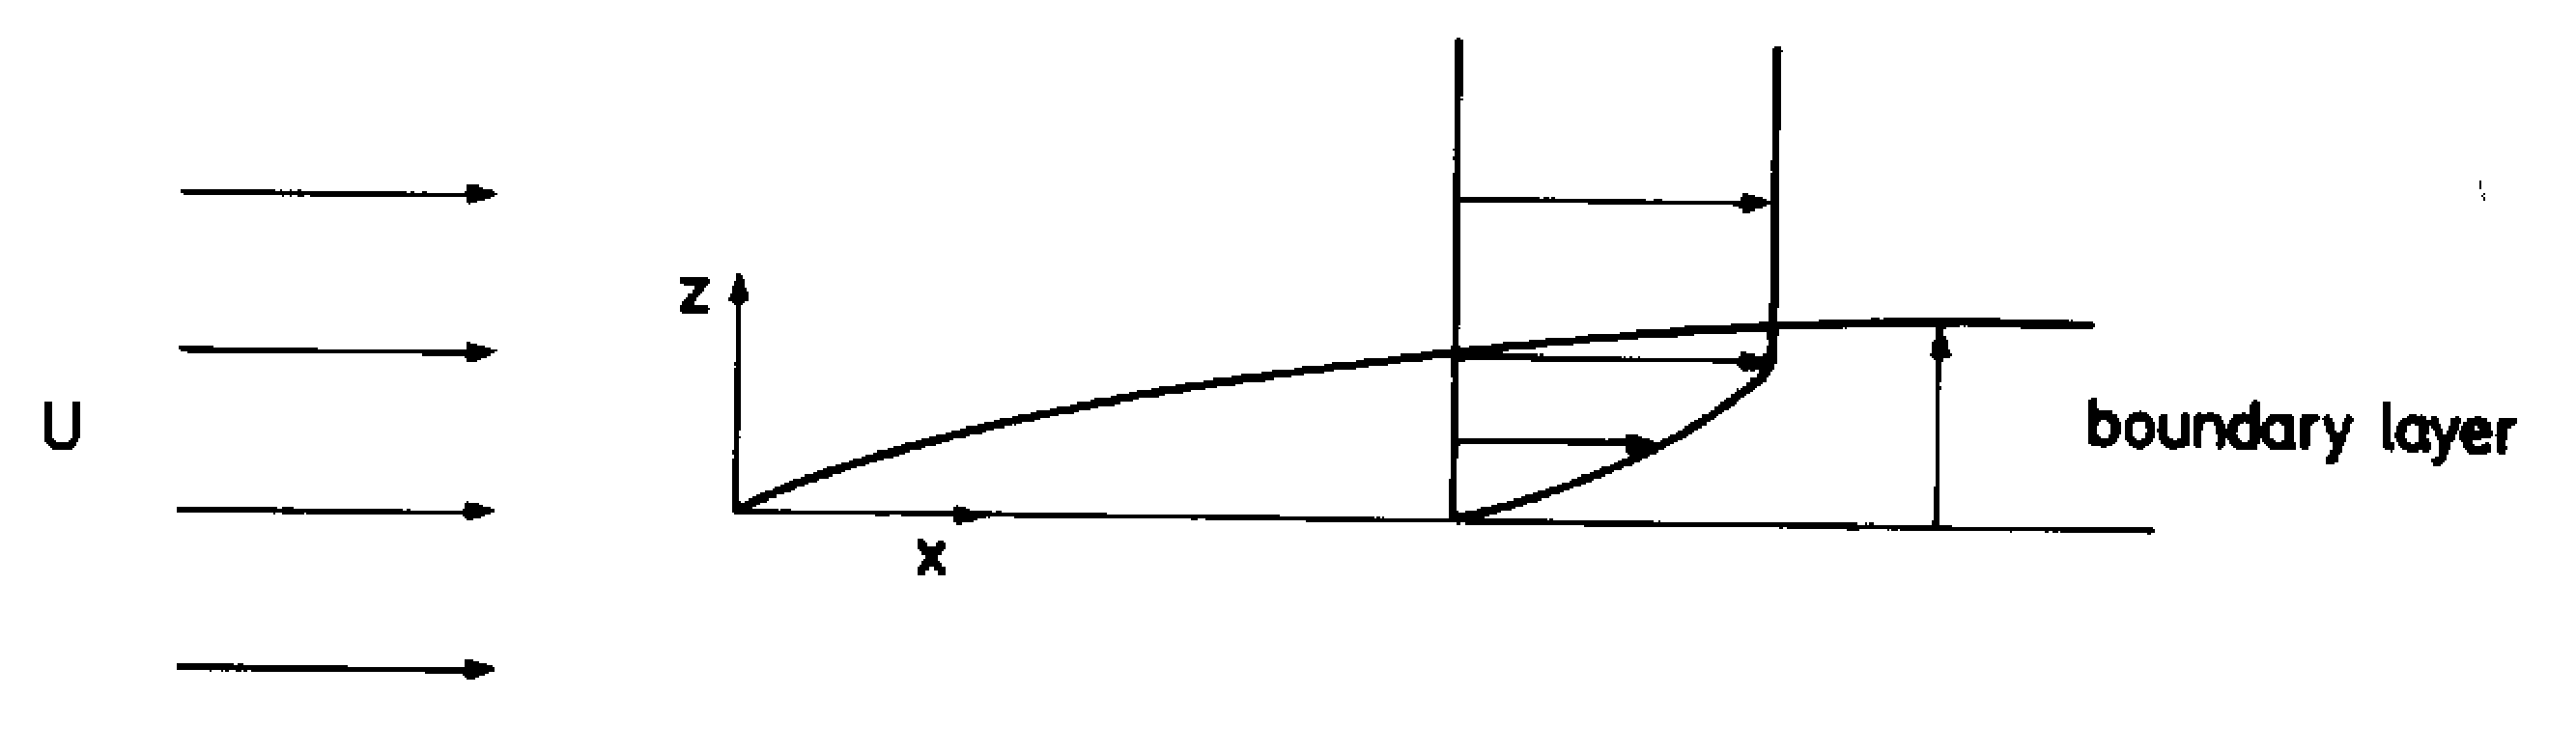
\includegraphics[width=4in]{Section61.pdf}}
\label{fig1}
\end{figure}

We consider the boundary layer on a flat plate at normal incidence to a 
uniform stream $U$ as shown.

The Navier Stokes' equations for steady two-dimensional flow with typical 
scales written below each component are:
\begin{align}
& u\frac{\partial u}{\partial x}+w\frac{\partial u}{\partial 
z}=-\frac{1}{\rho }\frac{\partial p}{\partial x}+\nu 
\left( {\frac{\partial ^2u}{\partial x^2}+\frac{\partial 
^2u}{\partial z^2}} \right), \label{eq62} \\
& \ \  \frac{U^2}{L}
\quad 
\frac{UW}{H}
\ \ \qquad
\frac{\Delta p}{\rho L}
\quad \qquad
\nu \frac{U}{L^2}
\quad
\nu \frac{U}{H^2} \notag
\end{align}
\begin{align}
& u\frac{\partial w}{\partial x}+w\frac{\partial w}{\partial 
z}=-\frac{1}{\rho }\frac{\partial p}{\partial z}+\nu 
\left( {\frac{\partial ^2w}{\partial x^2}+\frac{\partial 
^2w}{\partial z^2}} \right)\quad , \label{eq64} \\
&\  \frac{UW}{L}
\ \ \quad
\frac{W^2}{H}
\qquad
\frac{\Delta p}{\rho H}
\qquad \quad
\nu \frac{W}{L^2}
\quad
\nu \frac{W}{H^2} \notag
\end{align}
and the continuity equation is
\begin{align}
& \frac{\partial u}{\partial x}+\frac{\partial w}{\partial 
z}=0. \label{eq66} \\
& \ \frac{U}{L}
\ \quad
\frac{W}{H} \notag
\end{align}
From the continuity equation we conclude that since $\left| {{\partial u} 
/ {\partial x}} \right|=\left| {{\partial w} 
/ {\partial z}} \right|$, $W \sim UH/L$ and hence 
the two advection terms on the left hand sides of (\ref{eq62}) and (\ref{eq64}) are the 
same order of magnitude: $U^{2}/L$ in (\ref{eq62}) and $(U^{2}/L) (H/L)$ in 
(\ref{eq64}). Now, for a thin boundary layer, $H/L \ll 1$ so that the derivatives 
$\partial ^{2}/\partial x^{2 }$ in (\ref{eq62}) and (\ref{eq64}) can be neglected 
compared with $\partial ^{2}/\partial x^{2 }$. Then in (\ref{eq62}), assuming 
that the pressure gradient term is not larger than both inertial or friction 
terms\footnote{ Note that if this were not true, steady flow would not be 
possible as the large pressure gradient would accelerate the flow further.}, 
we have
\[
\frac{U^2}{L}\sim \nu \frac{U}{H^2}\ge \frac{\Delta p}{\rho L}.
\]
The first two terms imply that $H \sim L\ Re^{-1/2}$. Alternatively, this 
expression implies that the boundary thickness increases downstream like 
$x^{1/2}$ [i.e., $H \sim L^{1/2} (\nu /U)^{1/2}$]. Now from (\ref{eq64}) we 
find that
\begin{gather*}
{\frac{\Delta p}{\rho H}} / {\frac{UW}{L}}\sim 
{\frac{\rho U^2}{\rho H}} / 
{\frac{U^2H}{L^2}}\sim \frac{L^2}{H^2}>>1 \\
{\frac{\Delta p}{\rho H}} / {\frac{\nu 
W}{H^2}}\sim {\frac{\rho U^2}{\rho H}} /{\frac{\nu U}{HL}}\sim \frac{UL}{\nu }=Re>>1.
\end{gather*}
But if both the inertia terms and friction terms in (\ref{eq64}) are much less than 
the pressure gradient term, the equation must be accurately approximated by
\[
\frac{\partial p}{\partial z}=0.
\]
This implies that the perturbation pressure is constant across the boundary 
layer. It follows that the horizontal pressure gradient in the boundary 
layer is equal to that in free stream.

Collecting these results together we find that an approximate form of the 
Navier-Stokes' equations for the boundary layer to be
\begin{equation}
\label{eq67a}
u\frac{\partial u}{\partial x}+w\frac{\partial u}{\partial 
z}=U\frac{dU}{dx}+\nu \frac{\partial ^2u}{\partial z^2}\quad ,
\end{equation}
with 
\begin{equation}
 \frac{\partial u}{\partial x}+\frac{\partial w}{\partial z}=0, \label{eq67b}  
\end{equation}
and $U = U(x)$ being the (possible variable) free stream velocity above the 
boundary layer. Equations (\ref{eq67a}) and (\ref{eq67b}) are called the \textbf{boundary 
layer equations}.

\section{Blasius' solution ($U$ = constant)}
Equation (\ref{eq67a}) reduces to
\begin{equation}
\label{eq68}
u\frac{\partial u}{\partial x}+w\frac{\partial u}{\partial z}=\nu 
\frac{\partial ^2u}{\partial z^2}\quad ,
\end{equation}
and we look for a solution satisfying the boundary conditions $u = 0$, $w = 0$ 
at $z = 0$, $u \to  U$ as $z \to \infty $ and $u = U$ at $x = 0$. Equation (\ref{eq67b}) 
suggests that we introduce a streamfunction $\psi $ such that
\[ u=\frac{\partial \psi }{\partial z}, \quad w=-\frac{\partial \psi }{\partial 
x}, \]
whereupon $\psi $ must satisfy the conditions $\psi $ = constant, $\partial 
\psi /\partial z = 0$ at $z = 0$, $\psi  \sim  Uz$ as $z \to \infty $ 
and $\psi  = Uz$ at $x = 0$. It is easy to verify that a solution satisfying 
these conditions is
\begin{equation}
\label{eq69}
\psi =\left( {2\nu Ux} \right)^{\textstyle{1 \over 2}}f\left( \chi \right),
\end{equation}
where
\begin{equation}
\label{eq610}
\chi =\left( {U/ {2\nu x}} \right)^{\textstyle{1 \over 2}}z,
\end{equation}
and $f(\chi )$ satisfies the ordinary differential equation
\begin{equation}
\label{eq611}
{f}'''+f{f}''=0,
\end{equation}
subject to the boundary conditions
\begin{equation}
f(0) = f'(0) = 0; \quad f'(\infty ) = 1 . \label{eq613} \end{equation}

\begin{wrapfigure}{r}{3in}
\centerline{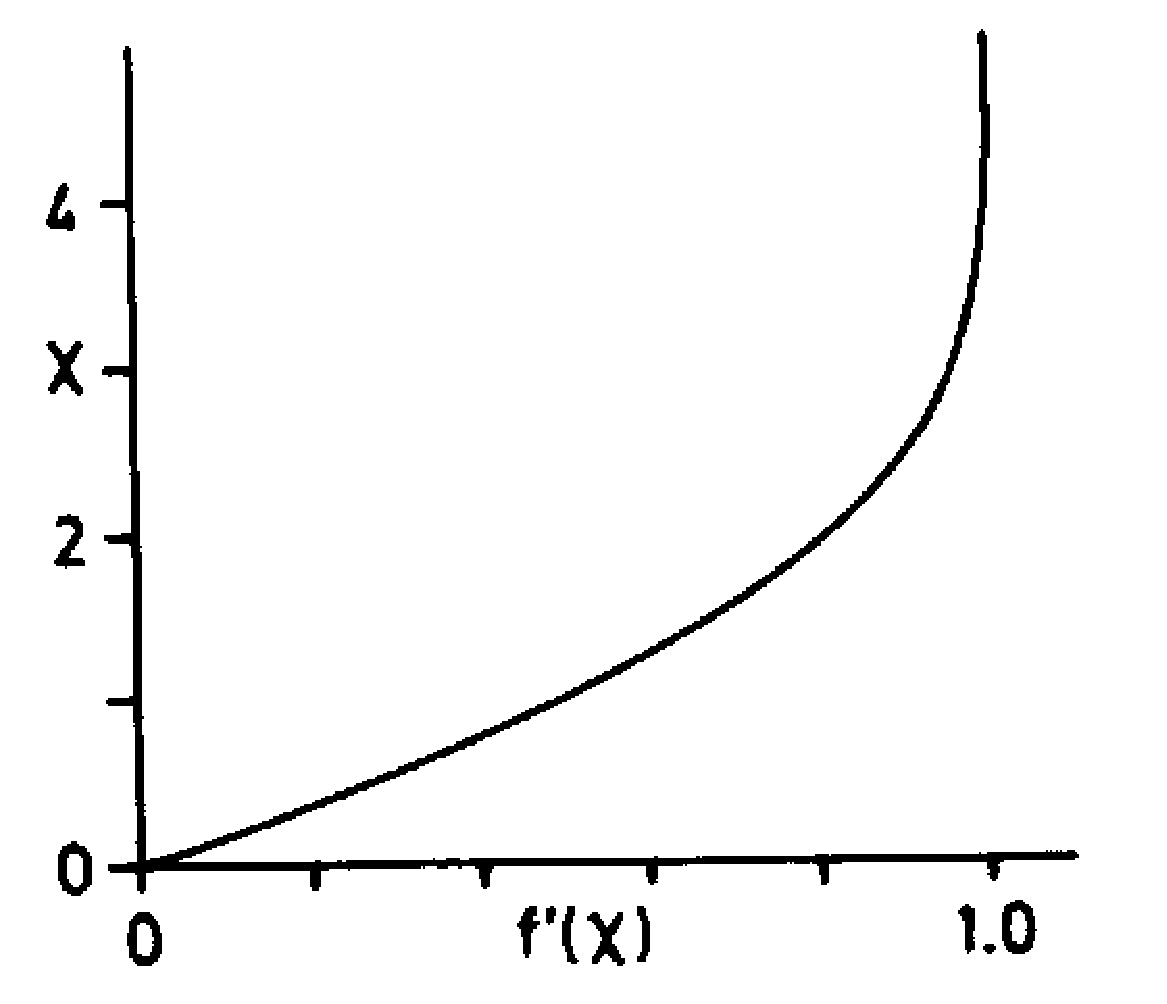
\includegraphics[width=3in]{Section62.pdf}}
\label{fig2}
\end{wrapfigure}

Here, a prime denotes differentiation with respect to $\chi $. It is easy to 
solve Eq. (\ref{eq611}) subject to (\ref{eq613}) numerically (see e.g. Rosenhead, 1966, 
\textit{Laminar Boundary Layers}, p. 222-224). The profile of $f'$ which characterizes the variation of $u$ 
across the boundary layer thickness is proportional to $\chi $ and we might 
take $\chi  = 4$ as corresponding with the edge of the boundary layer. Then 
(\ref{eq610}) shows that the dimensional boundary thickness $\delta \left( x 
\right)=4(2\nu x/ U)^{\textstyle{1 \over 2}}$, i.e., 
increases like the square root of the distance from the leading edge of the 
plate. We can understand the thickening of the boundary layers as due to the 
progressive retardation of more and more fluid as the fictional force acts 
over a progressively longer distance downstream.

Note that the boundary layer is \textbf{rotational} since ${\bm\omega}
= (0, \eta , 0)$, where $\eta ={\partial u} / {\partial 
z-}{\partial w}/{\partial x}$, or approximately just 
${\partial u}/ {\partial z}$. 

Often the boundary layer is relatively thin. Consider for example the 
boundary layer in an aeroplane wing. Assuming the wing to have a span of 3 m 
and that the aeroplane flies at 200 ms$^{-1}$, the boundary layer at the 
trailing edge of the wing (assuming the wing to be a flat plate) would have 
thickness of 4(2 $\times $ 1.5 $\times $ 10$^{-5 }\times $ 3/200)$^{1/2}$ 
= 2.7 $\times $ 10$^{-3}$ m using the value $\nu $ = 1.5 $\times $ 10$^{-5}$ 
m$^{2}$s$^{-1}$ for the viscosity of air. The calculation assumes that the 
boundary layer remains laminar; if it becomes turbulent, the random eddies 
in the turbulence have a much larger effect on the lateral momentum transfer 
than do random molecular motions, thereby increasing the effective value of 
$\nu $, possibly by an order of magnitude or more, and hence the boundary 
layer thickness.

\subsection*{Exercises}
\begin{enumerate}
\item Define the Reynolds number and explain its physical significance. 
Estimate the Reynolds number for a ball of radius 10 cm thrown at a speed of 
15 ms$^{-1}$. The kinematic viscosity for air is 1.5$\times $10$^{-5}$ 
m$^{2}$s$^{-1}$.
\end{enumerate}

\chapter{Two Dimensional Flow Past a Cylinder}
In two dimensions $(x, z)$, the Euler equations of motion are
\begin{align}
& \frac{\partial u}{\partial t}+u\frac{\partial u}{\partial 
x}+w\frac{\partial u}{\partial z}=-\frac{1}{\rho }\frac{\partial 
p}{\partial x}\quad , \label{eq71} \\
& \frac{\partial w}{\partial t}+u\frac{\partial w}{\partial 
x}+w\frac{\partial w}{\partial z}=-\frac{1}{\rho }\frac{\partial 
p}{\partial z}\quad , \label{eq72}
\end{align}
and the continuity equation is
\begin{equation}
\label{eq73}
\frac{\partial u}{\partial x}+\frac{\partial w}{\partial z}=0 .
\end{equation}
The vorticity ${\bm\omega}$ has only one non-zero component, the 
$y$-component, i.e., ${\bm\omega}= (0, \eta , 0)$, where
\begin{equation}
\label{eq74}
\eta =\frac{\partial u}{\partial z}-\frac{\partial w}{\partial x}.
\end{equation}
Taking ($\partial /\partial z$)(\ref{eq71}) - ($\partial /\partial x$)(\ref{eq72}) and 
using the continuity equation we can show that 
\begin{equation}
\label{eq75}
\frac{D\eta }{Dt}=0.
\end{equation}
This equation states that fluid particles conserve their vorticity as they 
move around. This is a powerful and useful constraint. In some problems, 
$\eta  = 0$ for all particles. Such flows are called \textbf{irrotational}.

\section{Flow past a cylinder without circulation}
Consider, for example, the steady flow around a cylinder.  All fluid particles originate from far upstream ($x 
\to -\infty )$ where $u = 0$, $w = 0$,
and therefore $\eta  = 0$. It follows that fluid particles have zero 
vorticity for all time.

\begin{figure}[htbp]
\centerline{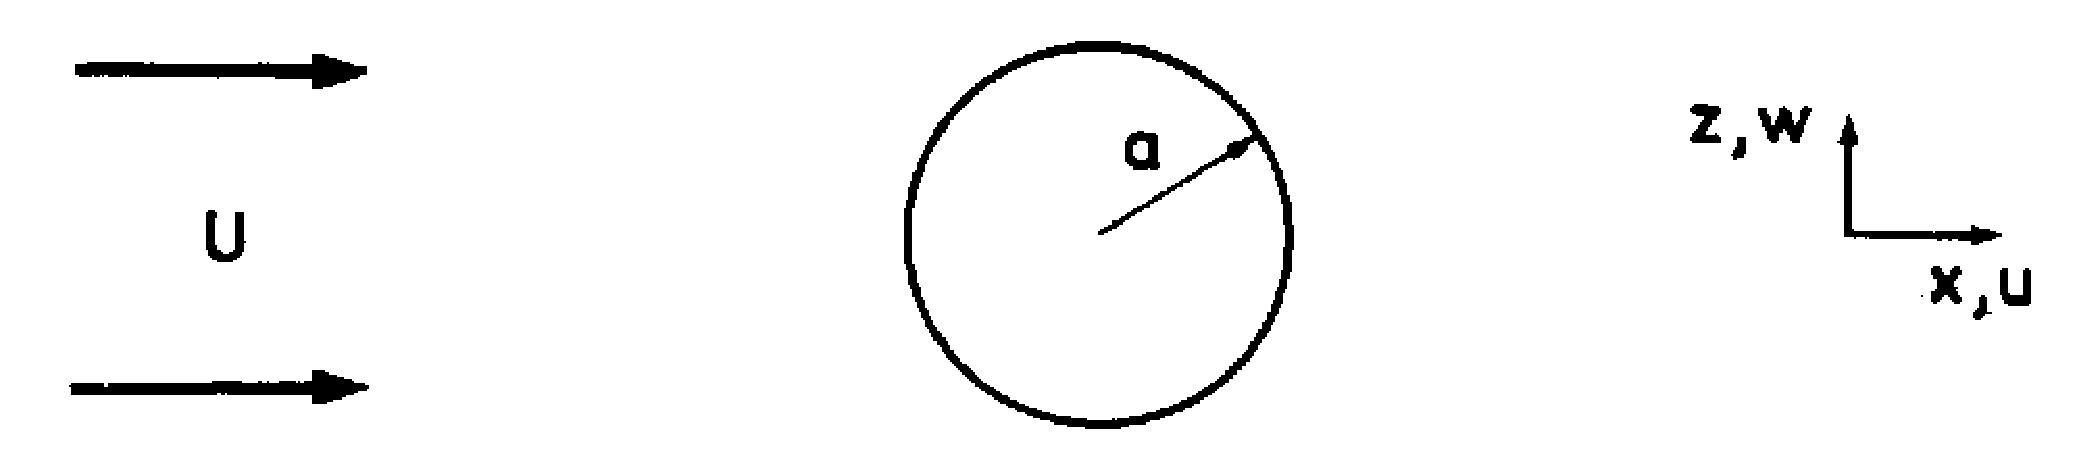
\includegraphics[width=4in]{Section71.pdf}}
\label{fig1}
\end{figure}

The inviscid flow problem can be solved as follows. Note that the continuity 
equation (\ref{eq73}) suggests that we introduce a \textbf{streamfunction} $\psi $, 
defined by the equations 
\[ u=\frac{\partial \psi }{\partial z}, \quad w=-\frac{\partial \psi }{\partial 
x}. \label{eq76} \]

Then (\ref{eq75}) is automatically satisfied and it follows from (\ref{eq74}) that
\begin{equation}
\eta =\frac{\partial ^2\psi }{\partial x^2}+\frac{\partial ^2\psi 
}{\partial z^2}\quad .
\end{equation}
In the case of \textbf{irrotational flow}, $\eta $ = 0 and $\psi $ satisfies 
Laplace's equation
\begin{equation}
\label{eq77}
\frac{\partial ^2\psi }{\partial x^2}+\frac{\partial ^2\psi }{\partial 
z^2}=0\quad .
\end{equation}

Appropriate boundary conditions are found using (7.6). For example, on a 
solid boundary, the normal velocity must be zero, i.e., $ \textbf{u} . 
\textbf{n} = 0$ on the boundary. If $ \textbf{n} = (n_{1}, 0, n_{3})$, it 
follows using (\ref{eq76}) that $n_1 {\partial \psi } /
{\partial z-n_3 } / {\partial x}=0$, or 
$\textbf{n} \times  \nabla \psi $ = \textbf{0} on the boundary. We 
deduce that $\nabla \psi $ is in the direction of  $\textbf{n}$, whereupon 
$\psi $ is a constant on the boundary itself.

\begin{figure}[htbp]
\centerline{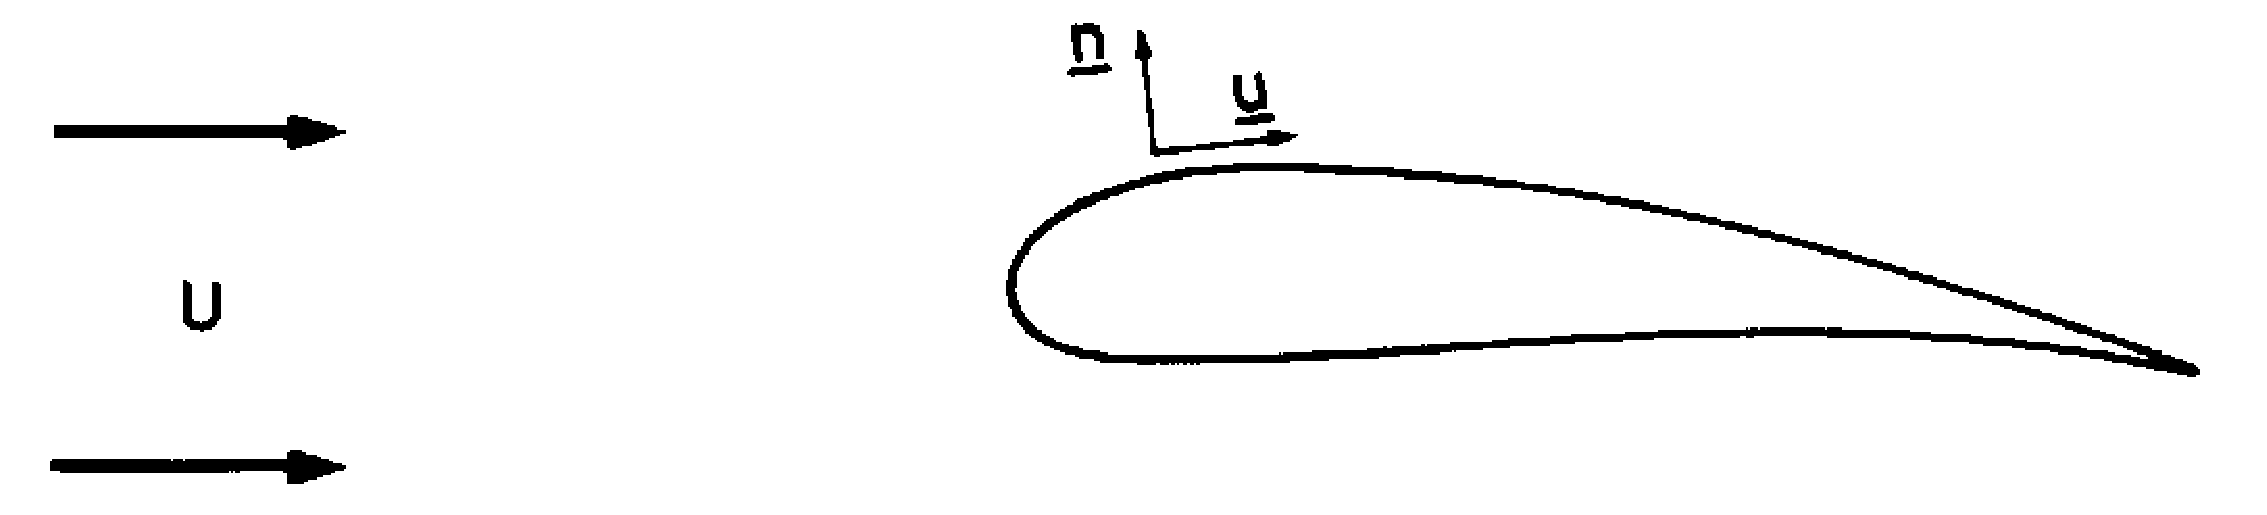
\includegraphics[width=4in]{Section72.pdf}}
\label{fig2}
\end{figure}

Let us return to the example of uniform flow past a cylinder of radius $a$: 

\begin{figure}[htbp]
\centerline{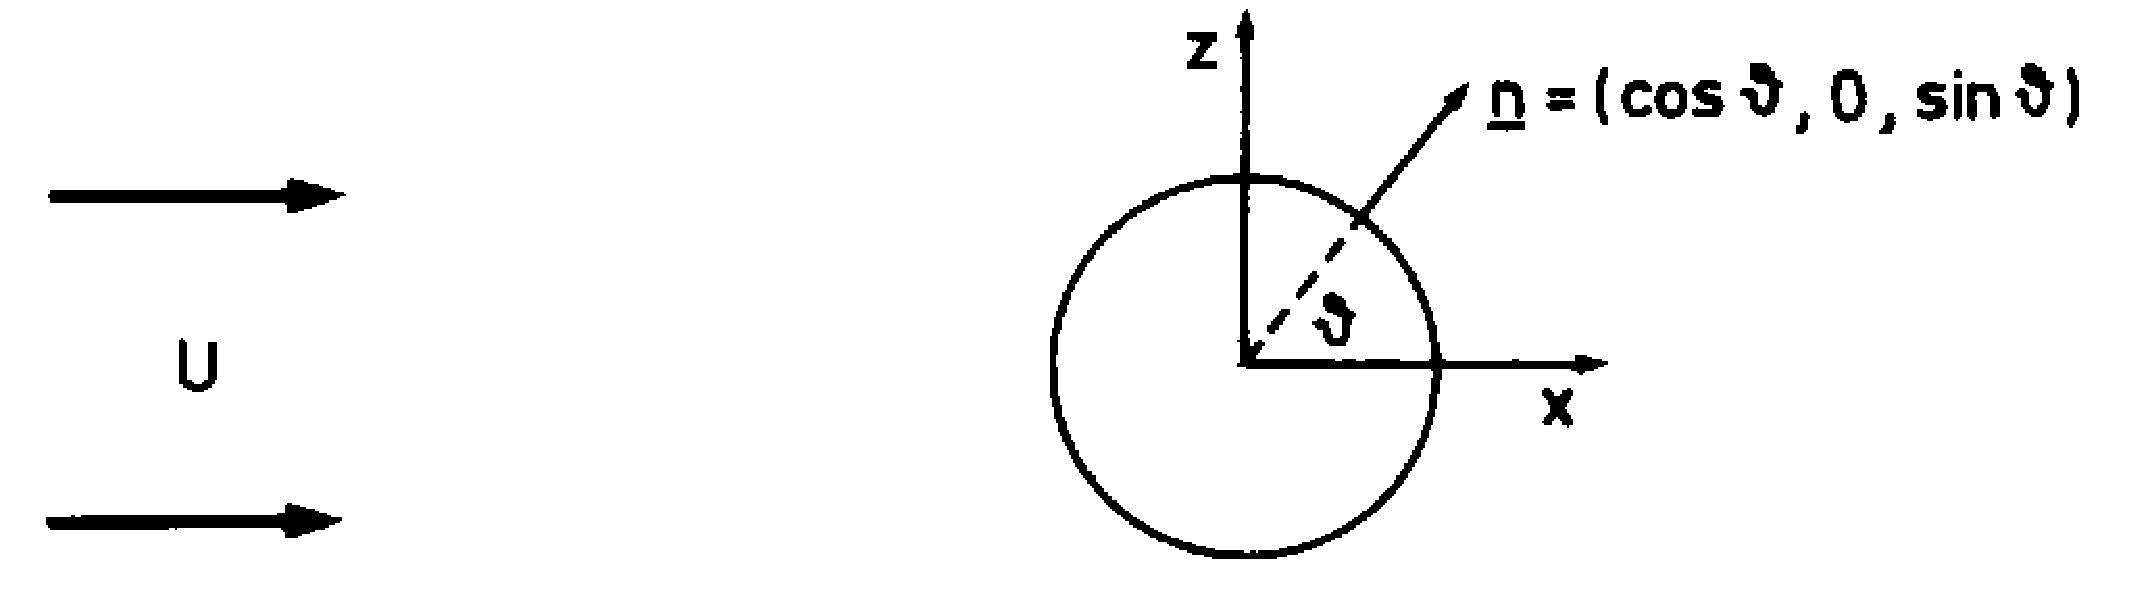
\includegraphics[width=4in]{Section73.pdf}}
\label{fig3}
\end{figure}

The problem is to solve (\ref{eq77}) in the region outside the cylinder (i.e. $ r 
> a$) subject to the boundary condition that
\begin{equation}
\label{eq78}
{{\bf u}}=\left( {\frac{\partial \psi }{\partial z},0,-\frac{\partial 
\psi }{\partial x}} \right)\to \left( {U,0,0} \right)\quad\hbox{as}\quad r\to \infty 
\quad ,
\end{equation}
and 
\begin{equation} {{\bf u}}. {{\bf n}}=0\quad \hbox{on}\quad r=a, \label{eq710} \end{equation}
where $r=\sqrt {x^2+z^2} $. For this problem it turns out to be easier to 
work in cylindrical polar coordinates centred on the cylinder. Since $x = r$ 
$\cos \theta $ and $z = r \sin \theta $, we can show that $\partial 
r/\partial x = \cos\theta $, $\partial r/\partial z = \sin\theta $, 
$\partial \theta /\partial x = -(\sin \theta )/r$ and $\partial 
\theta /\partial z = (\cos \theta )/r$.
Then 
\begin{align} \frac{\partial \psi }{\partial z}= & \frac{\partial \psi }{\partial 
r}\frac{\partial r}{\partial z}+\frac{\partial \psi }{\partial \theta 
}\frac{\partial \theta }{\partial z}, \notag \\
= & \sin \theta \frac{\partial \psi 
}{\partial r}+\frac{\cos \theta }{r}\frac{\partial \psi }{\partial \theta }. \label{eq711} \end{align}
Similarly, 
\begin{align} \frac{\partial \psi }{\partial x} & =\frac{\partial \psi }{\partial 
r}\frac{\partial r}{\partial x}+\frac{\partial \psi }{\partial \theta 
}\frac{\partial \theta }{\partial x}, \notag \\
& =\cos \theta 
\frac{\partial \psi }{\partial r}-\frac{\sin \theta }{r}\frac{\partial \psi 
}{\partial \theta }. \label{eq712} \end{align}

One can use (\ref{eq711}) and (\ref{eq712}) to transform (\ref{eq77}) to cylindrical polar 
coordinates giving,
\begin{equation}
\label{eq79}
\frac{1}{r}\left[ {\frac{\partial }{\partial r}\left( {r\frac{\partial 
\psi }{\partial r}} \right)+\frac{1}{r}\frac{\partial ^2\psi 
}{\partial \theta ^2}} \right]=0\quad .
\end{equation}
The boundary condition on the cylinder expressed by (\ref{eq710}) requires that
\[
\cos \theta \frac{\partial \psi }{\partial z}-\sin \theta \frac{\partial 
\psi }{\partial x}=0
\]
at $r = a$ and for all $\theta $. Using (\ref{eq711}) and (\ref{eq712}), this reduces to
\[ \frac{\partial \psi }{\partial \theta }=0 \quad \hbox{at}\quad  r = a. \label{eq714} \]
This equation implies that $\psi $ is a constant on the cylinder; i.e. the 
surface of the cylinder must be a streamline. Note also that for large $r$, 
$u = \partial \psi /\partial z \sim  U$ and hence 
\begin{equation}
\psi  \sim Uz = 
Ur \sin \theta . \label{eq715} \end{equation}

The far field solution (\ref{eq715}) suggests seeking separable solutions to (\ref{eq79}) 
of the form $\psi =f\left( r \right)\sin \theta $. Upon substituting this 
expression into (\ref{eq79}), we get
\begin{equation}
\label{eq716}
r^2\frac{d^2f}{dr^2}+r\frac{df}{dr}-f=0.
\end{equation}
Equation (\ref{eq716}) is an Euler--Cauchy equation and can be solved by seeking 
solutions of the form $f=r^k$, whereupon we find that $ k = \pm  1$. Hence,
\[
f(r)=c_1 r+\frac{c_2 }{r}.
\]
Apply the boundary conditions (\ref{eq78}) and (\ref{eq710}) shows that $c_{1} = U$ and 
$c_{2} = -Ua^{2}$, and consequently
\begin{equation}
\label{eq717}
\psi =U\left( {r-\frac{a^2}{r}} \right)\sin \theta .
\end{equation}
Note that $\psi  = 0$ on the cylinder. However, the solution for 
$\psi $ is unique only to within a constant value; if we add any constant to 
it, it will satisfy equation (\ref{eq77}) or (\ref{eq79}), but the velocity field would 
be unchanged.

In cylindrical polar coordinates the radial and tangential components of
velocity, $v_{r}$ and $v_{\theta }$, are related to the streamfunction by 
\[
v_r =\frac{1}{r}\frac{\partial \psi }{\partial \theta }\quad 
\hbox{and} \quad v_\theta =-\frac{\partial \psi }{\partial r}, 
\] 
Hence, from (\ref{eq11}), 
\[
v_r =Ur\left( {1-\frac{a^2}{r^2}} \right)\cos \theta \quad \hbox{and} \quad
v_\theta =-U\left( {1+\frac{a^2}{r^2}} \right)\sin \theta . 
\]
On the boundary
of the cylinder ($r = a$) $v_{r} = 0$ and $v_{\theta } = -2U\sin \theta $.

Recall that $v_{\theta }$ is positive when the flow is anticlockwise. For
example, on the top of the cylinder ($\theta =\pi /2$) the tangential velocity
is $v_{\theta } = -2U$, which is directed from left to right.

It is important to note that we have obtained a solution without reference to
the pressure field, but the pressure distribution determines the force field
that drives the flow! We seem, therefore, to have by-passed Newton's second
law, and have obviously avoided dealing with the nonlinear nature of the
momentum equations (\ref{eq71}) and (\ref{eq72}). Looking back we will see
that the trick was to use the vorticity equation, a derivative of the momentum
equations. For a homogeneous fluid, the vorticity equation does not involve
the pressure since $\nabla \times \nabla p \equiv $ 0. We infer from the
vorticity constraint, (\ref{eq75}), that the flow must be irrotational
everywhere and use this, together with the continuity constraint (which is
automatically satisfied when we introduce the streamfunction) to infer the
flow field. If desired, the pressure field can be determined, for example, by
integrating (\ref{eq71}) and (\ref{eq72}), or by using Bernoulli's equation
along streamlines.

\newpage
\begin{wrapfigure}{r}{3in}
\centerline{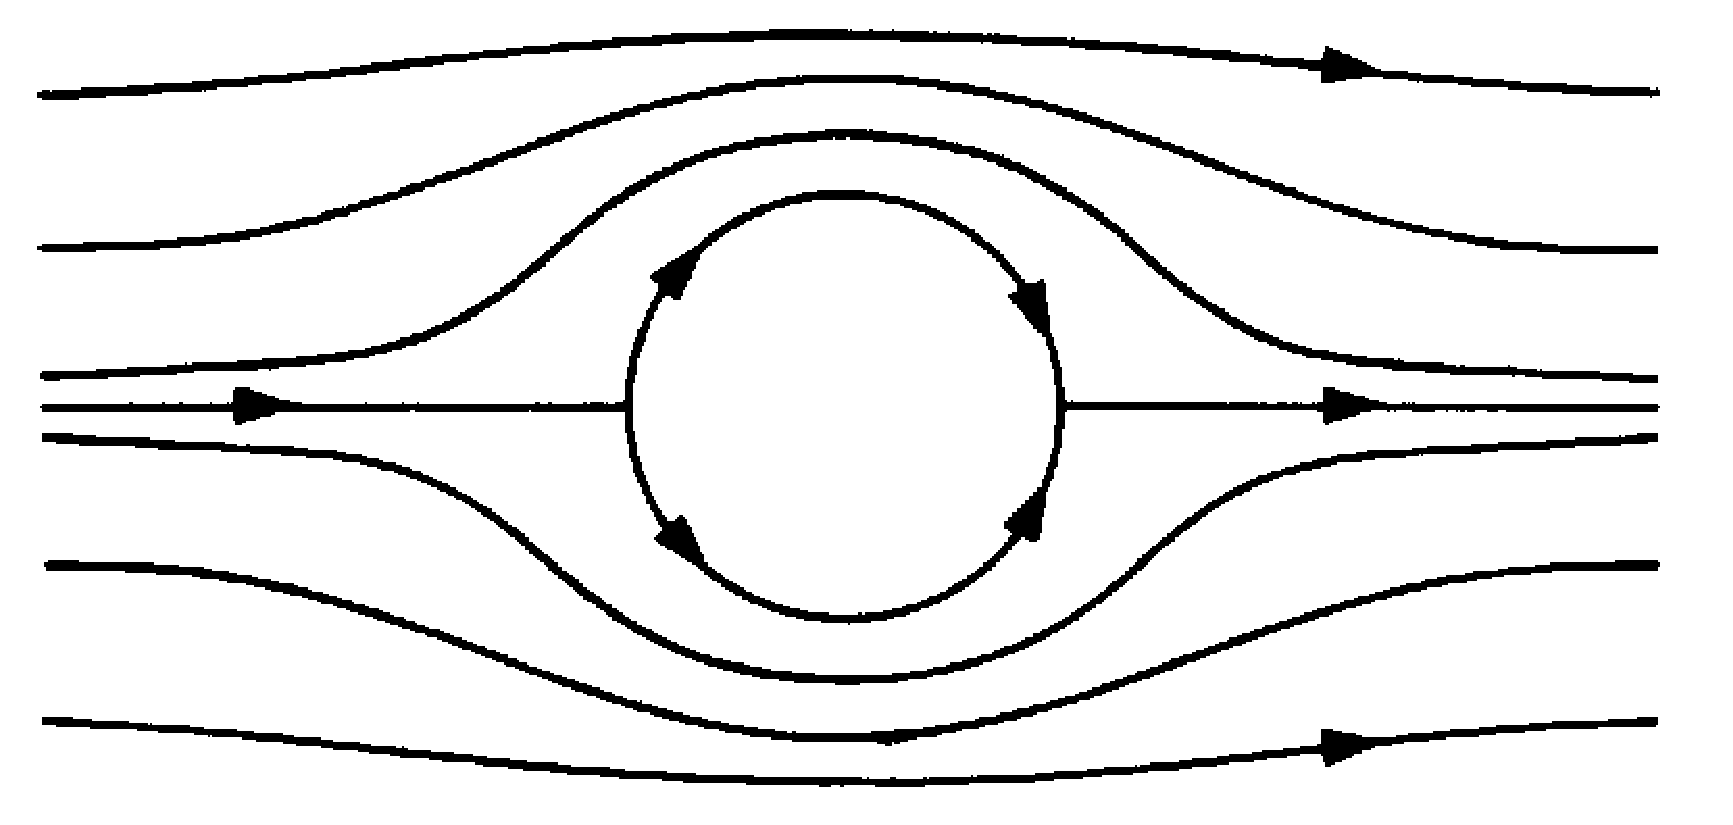
\includegraphics[width=3in]{Section74.pdf}}
\label{fig4}
\end{wrapfigure}

Now the solution itself. The streamline corresponding with (\ref{eq717}) are 
sketched. Note that they are symmetrical around the cylinder. Applying 
Bernoulli's equation to the streamline around the cylinder we find that the 
pressure distribution is symmetrical also so that the total pressure force 
on the upstream side of the cylinder is exactly equal to the pressure on the 
downwind side. In other words, the net pressure force on the cylinder is 
zero! This result, which in fact is a general one for irrotational inviscid 
flow past a body of any shape, is known as \textbf{d'Alembert's Paradox}. It 
is not in accord with our experience as you know full well when you try to 
cycle against a strong wind. What then is wrong with the theory? Indeed, 
what does the flow round a cylinder look like in reality? The reasons for 
the breakdown of the theory help us to understand the limitations of 
inviscid flow theory in general and help us to see the circumstances under 
which it may be applied with confidence. First, let us return to the viscous 
theory.

\begin{figure}[htbp]
\centerline{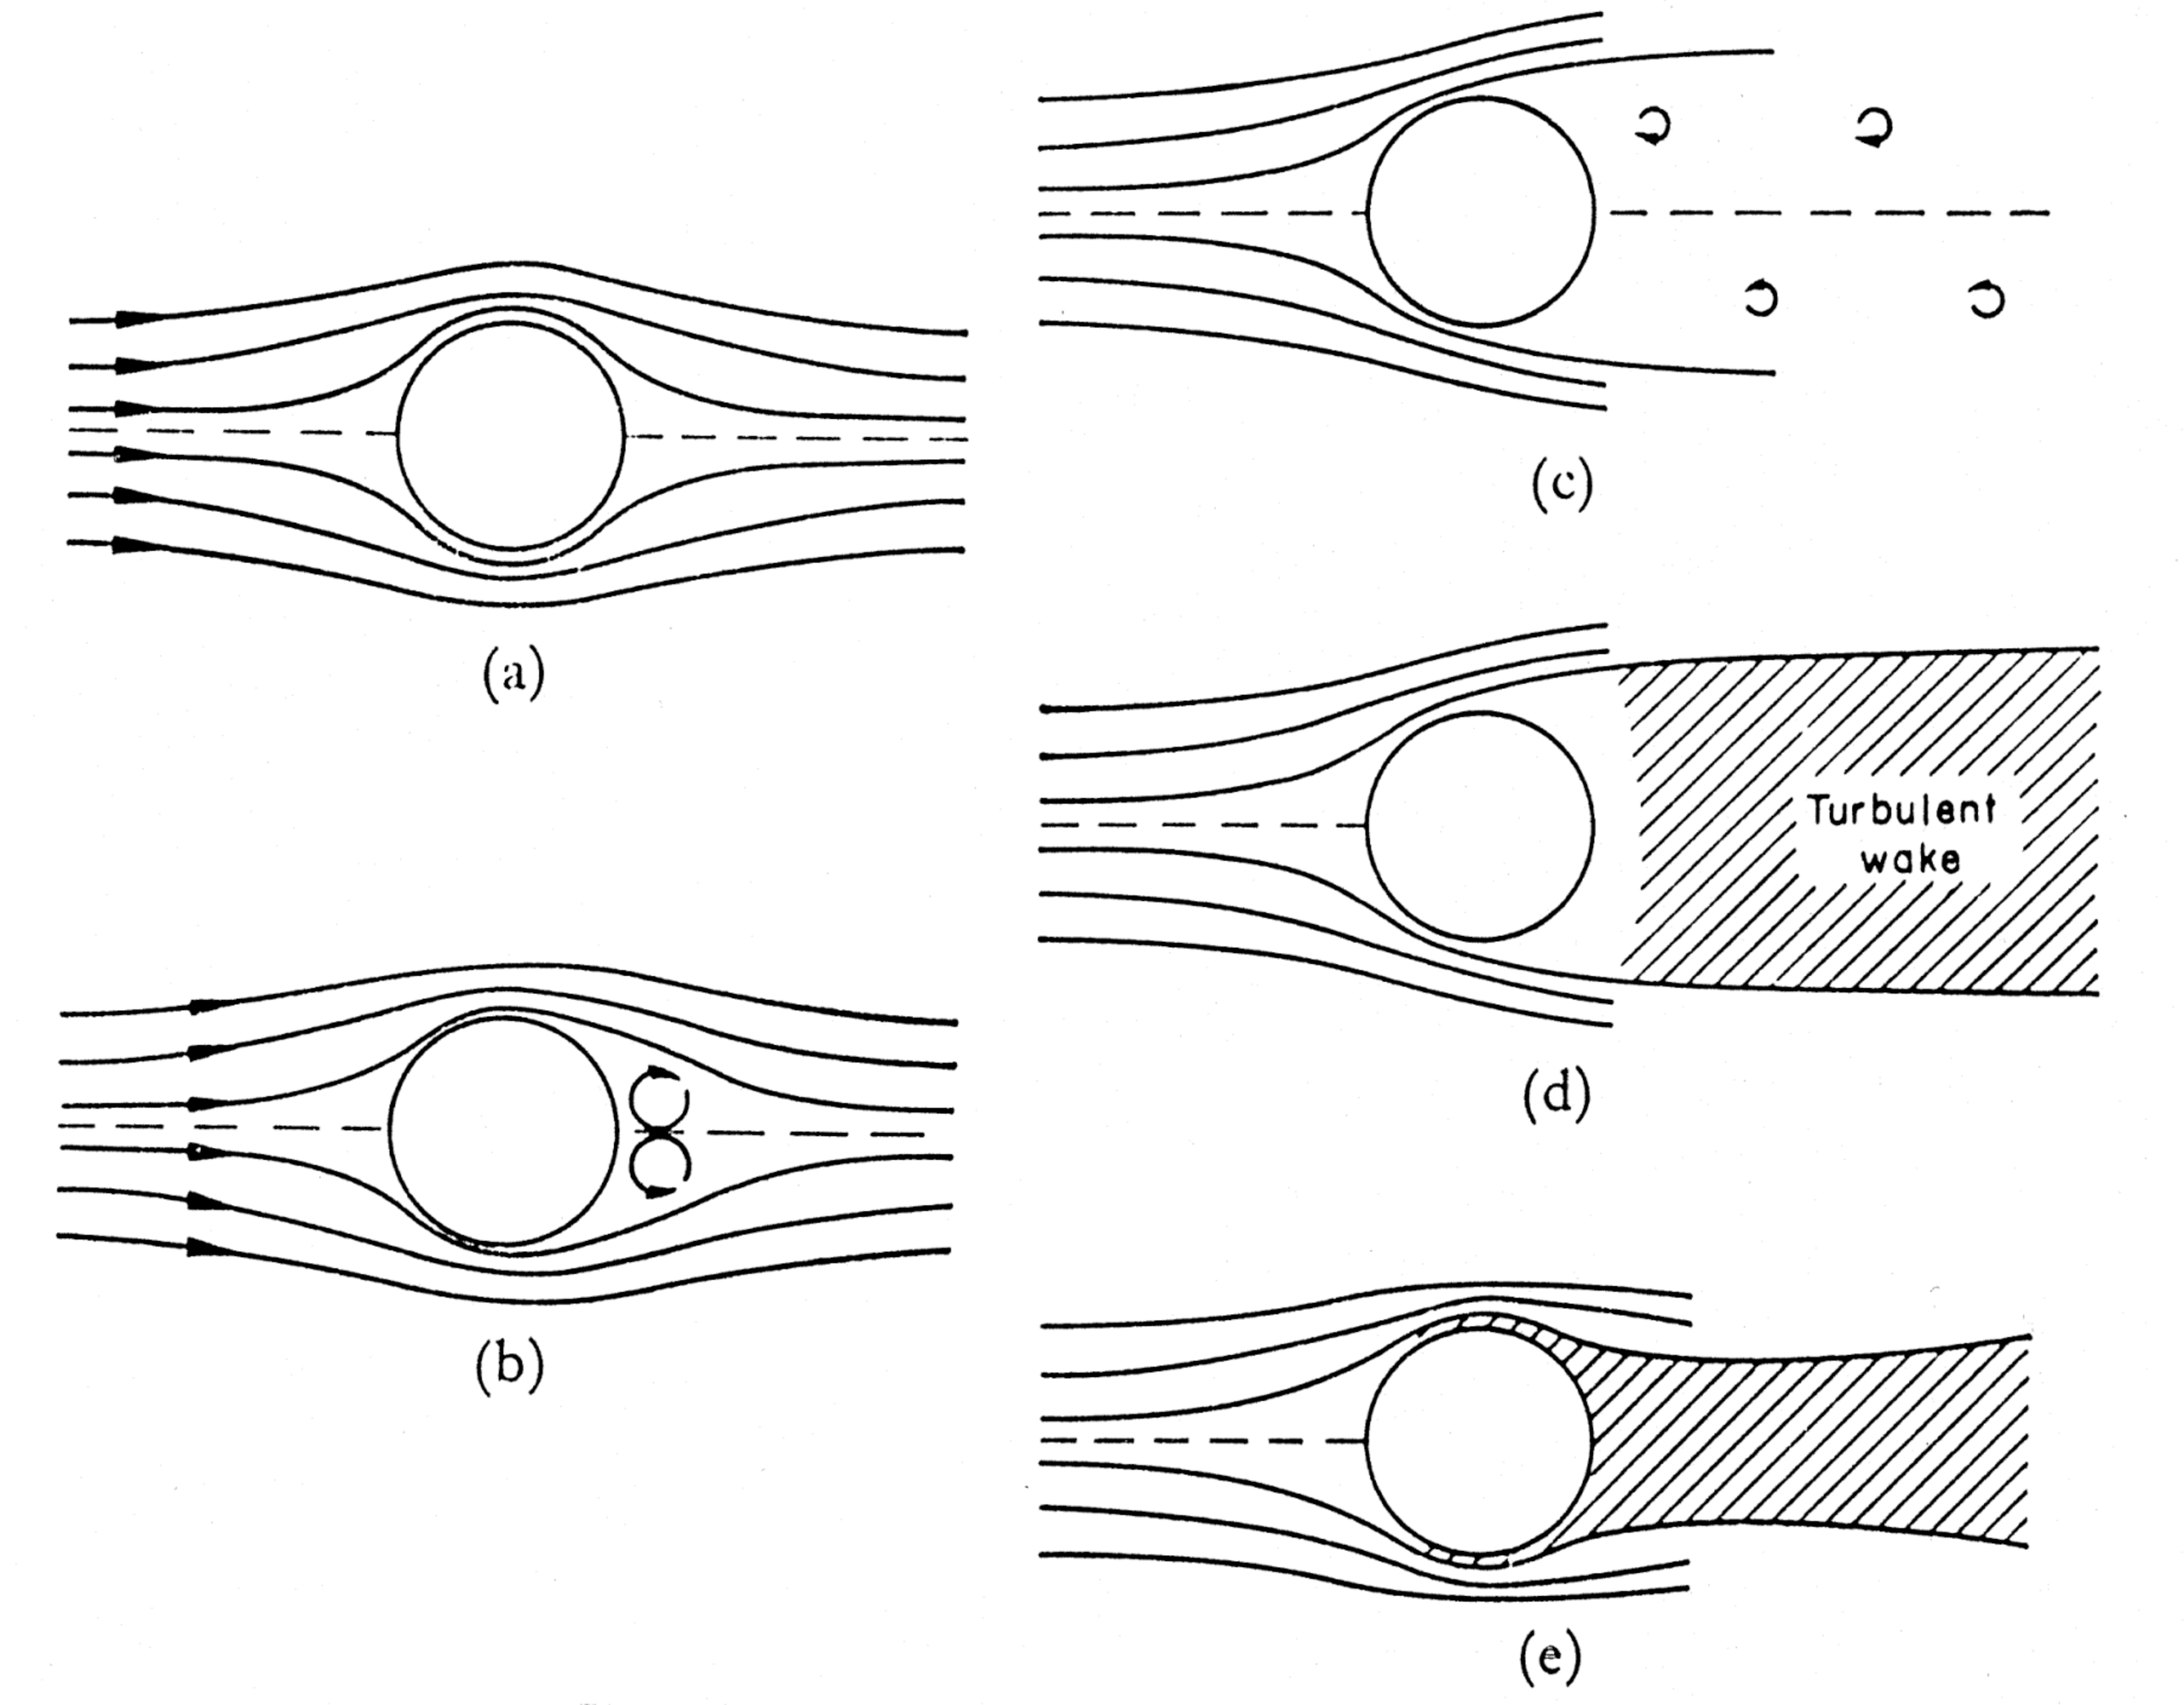
\includegraphics[width=5in]{Section75.pdf}}
{\bigskip}
\begin{center}
{Flow past a cylinder. (a) $Re < 1$. (b) $1< Re < 30$. (c) $40 < Re < 
4,000$. (d) $10^{3} < Re < 10^{5}$. (e) $Re > 10^{5}$. \\
{\small (From Modern Fluid Dynamics. Volume 1: Incompressible Flow, N. Curle
and H.J. Davies, 1967.)}}
\end{center}
\label{fig5}
\end{figure}



\section{Flow past a cylinder with friction}
The dynamics of the boundary layer plays a crucial role in flow past a 
circular cylinder. In particular it has important consequences for the solution downstream. 
The observed streamline pattern in this case at large Reynolds numbers is 
sketched in the figure below. The figure below shows how the flow past a 
cylinder changes with changing Reynolds number. Upstream of the cylinder the 
flow is similar to that predicted by the inviscid theory, except in a thin 
viscous boundary-layer adjacent to the cylinder. At points on the downstream 
side of the cylinder the flow separates and there is an unsteady turbulent 
wake behind it. For very small Reynolds number ($Re < 1$) viscosity is 
important, yet the flow is symmetrical and similar to the inviscid solution. 
As the Reynolds number increases ($1< Re < 30$) the flow behind the 
cylinder stretches out and two symmetrically-placed eddies form. For higher 
Reynolds number ($40 < Re < 4,000$), a time-dependent but ordered wake 
forms behind the cylinder (Karman vortex streets). This wake becomes 
turbulent as the Reynolds number increases further ($10^{3} < Re < 10^{5}$).
At very large Reynolds number ($Re > 10^{5}$) the turbulent
boundary layer reaches around the cylinder.

The existence of the wake destroys the symmetry in the pressure field 
predicted by the inviscid theory and there is net pressure force or 
\textbf{form drag} acting on the cylinder. Viscous stresses at the boundary 
itself cause additional drag on the body. However, as the Reynolds number 
increases from below about $Re > 10^{5}$, the drag drops sharply (which is 
critical for swing bowling). This is because the boundary layer becomes 
turbulent ahead of the separation point - more on this later.

\begin{figure}[htbp]
\centerline{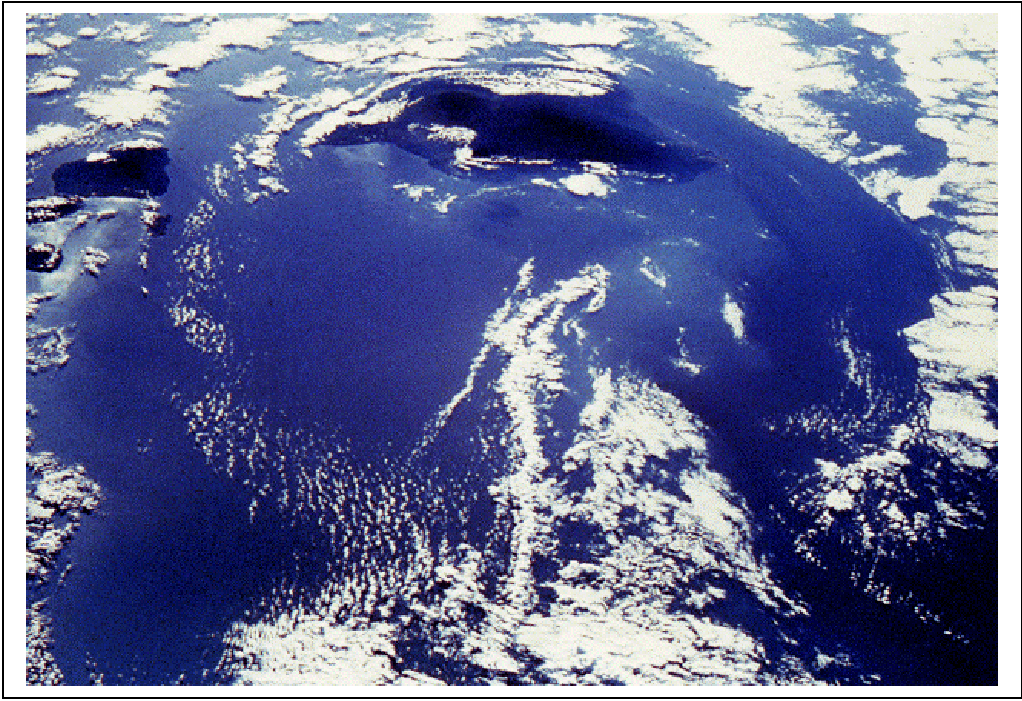
\includegraphics[width=3.5in]{Hawaii.jpg}}
\bigskip
\centerline{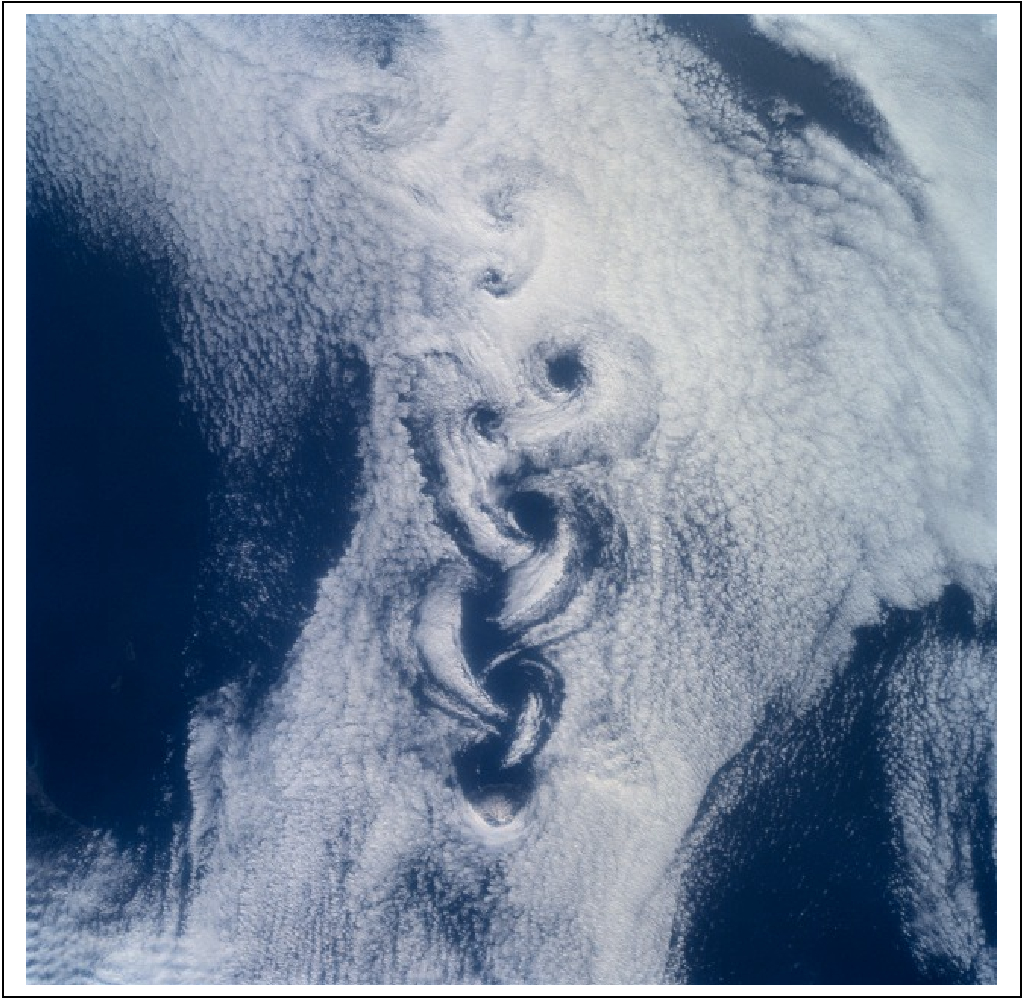
\includegraphics[width=3.5in]{island.jpg}}
{\bigskip}
\begin{center}
Examples of wakes in geophysical flows. Upper panel: a wake formed by airflow
around Hawaii. Lower panel: a Karmen vortex street formed in the lee of
volcanic island near Japan. {\small (From NASA.)}
\end{center}
\label{fig5}
\end{figure}

\section{Boundary Layer Separation}
If the Reynolds number is large, then the boundary layer may remain very 
thin and behave essentially like a vortex sheet. In this case the flow above 
the boundary layer may be well approximated by inviscid flow. However, under 
some circumstances the boundary layer separates from the solid boundary, in 
which case the interior flow may be radically different from that predicted 
by inviscid theory. For example, this is what happens when irrotational 
fluid flows around a cylinder. 

We investigate now the circumstances under which a boundary layer separates 
from the surface. The problem is mathematically very complex, so we will 
confine ourselves to a qualitative discussion of the key physical 
principles.

\newpage

\begin{wrapfigure}{r}{3in}
\centerline{\includegraphics[width=3in]{Section76.pdf}}
{\bigskip}
\begin{center}
{\small (From An Informal Introduction to Theoretical Fluid Mechanics, J. Lighthill, 1986.)}
\end{center}
\label{fig6}
\end{wrapfigure}

The figure to the right shows schematically the separation of a boundary layer around an 
elliptic cylinder at rest in an oncoming flow with velocity $U$. Assuming that 
the flow is irrotational outside the boundary layer, we can calculate the 
streamlines and velocity field using a method similar to that used in 
Section 7.1. The streamlines are shown in (a) and velocity just outside the 
boundary layer in shown in panel (b). Where the streamlines are compressed 
the stream speed is high and pressure is low (by Bernoulli's theorem). To 
the extent that the boundary layer can be treated as a vortex sheet, the 
strength ($\omega \delta )$ is largest where the velocity is largest. 

The flow accelerates, and the strength of the vortex sheet increases, along 
a streamline between points $A$ and $B$ (panel c). Consequently, vorticity is 
removed from $B$ faster than it is replaced from $A$. On the other hand 
vorticity of the \textbf{same sense} as the vortex sheet is generated at the 
boundary by the (negative) pressure gradient. In addition, the newly 
generated vorticity diffuses \textbf{slowly} away from the boundary. The 
relative importance of the tangential pressure gradient and diffusion to the 
circulation budget at the surface can be assessed by comparing $-\rho 
^{-1}{\partial p} / {\partial x}$ to $\nu {\partial ^2u} 
/ {\partial z^2}$. 

Between $C$ and $D$ a similar argument can be made with the necessary changes (panel d). 
Vorticity is 
advected to $D$ faster than it is advected away, but vorticity of the 
\textbf{opposite sign} to that in the vortex sheet is generated by the 
adverse (positive) pressure gradient between $C$ and $D$. Diffusion slowly 
transports the newly generated (negative) vorticity away from the surface 
into the boundary layer and transports (positive) boundary layer vorticity 
to the surface. Provided that negative vorticity is not generated too 
quickly by the boundary pressure gradient, diffusion will ensure that a 
reversed circulation does not develop at the solid surface. 

The flow is strongly retarded by the pressure gradient at $E$. Here the rate 
of diffusion is much smaller than the rate of generation by the pressure 
gradient, and circulation in the sense opposite to that in the boundary 
layer is generated. If the adverse pressure gradient is large enough the 
generation of negative vorticity may produce a local region wherein the 
vorticity changes sign. Consequently, the flow lifts off the surface (or 
\textbf{separates}) as shown in panel (e). Note that $\Delta p$ is \textbf{large} and 
positive at $E$; separation occurs only in regions of very strong adverse 
pressure gradient, and for this reason aircraft wings a highly tapered.

As the Reynolds number increases beyond about $10^{5}$ flows often become 
turbulent. Turbulence acts to prevent boundary layer separation by 
increasing the mixing in the boundary layer, effectively increasing the 
value of $\nu $. 

\section{Inviscid flow past a cylinder with circulation}
Consider, now the problem of a steady, inviscid, uniform flow $U$ past a 
cylinder of radius $a $ with circulation. We ignore the question of how the 
circulation was generated, which must involve the acceleration of the 
boundary relative to the interior flow and the subsequent diffusion of 
vorticity into the interior. 

The circulation is specified and we calculate the flow past the cylinder. As 
the problem is linear, the solution is just that for flow past a 
non-rotating cylinder and that for the line vortex,
\begin{equation}
\label{eq718}
\psi =Ur\left( {1-\frac{a^2}{r^2}} \right)\sin \theta +\frac{\kappa }{2\pi 
}\ln r\quad .
\end{equation}
Consequently, 
\[ v_\theta =-U\left( {1+\frac{a^2}{r^2}} \right)\sin \theta 
-\frac{\kappa }{2\pi r}, \label{eq719} \]
so that on the boundary of the cylinder ($r = a$), 
\begin{equation}
v_\theta =-U\sin \theta 
-\frac{\kappa }{2\pi a}. \label{eq720} \end{equation}
Equation (\ref{eq720}) shows two stagnation points occur on the surface of the 
cylinder when $B=\left| {\kappa / {\left( {4\pi Ua} 
\right)}} \right|<1$. These two points coalesce when $B = 1$. When $B > 1$, 
there are no stagnation points on the cylinder, although one occurs off the 
cylinder. The solution for various values of $B$ is shown below.

\begin{figure}[htbp]
\centerline{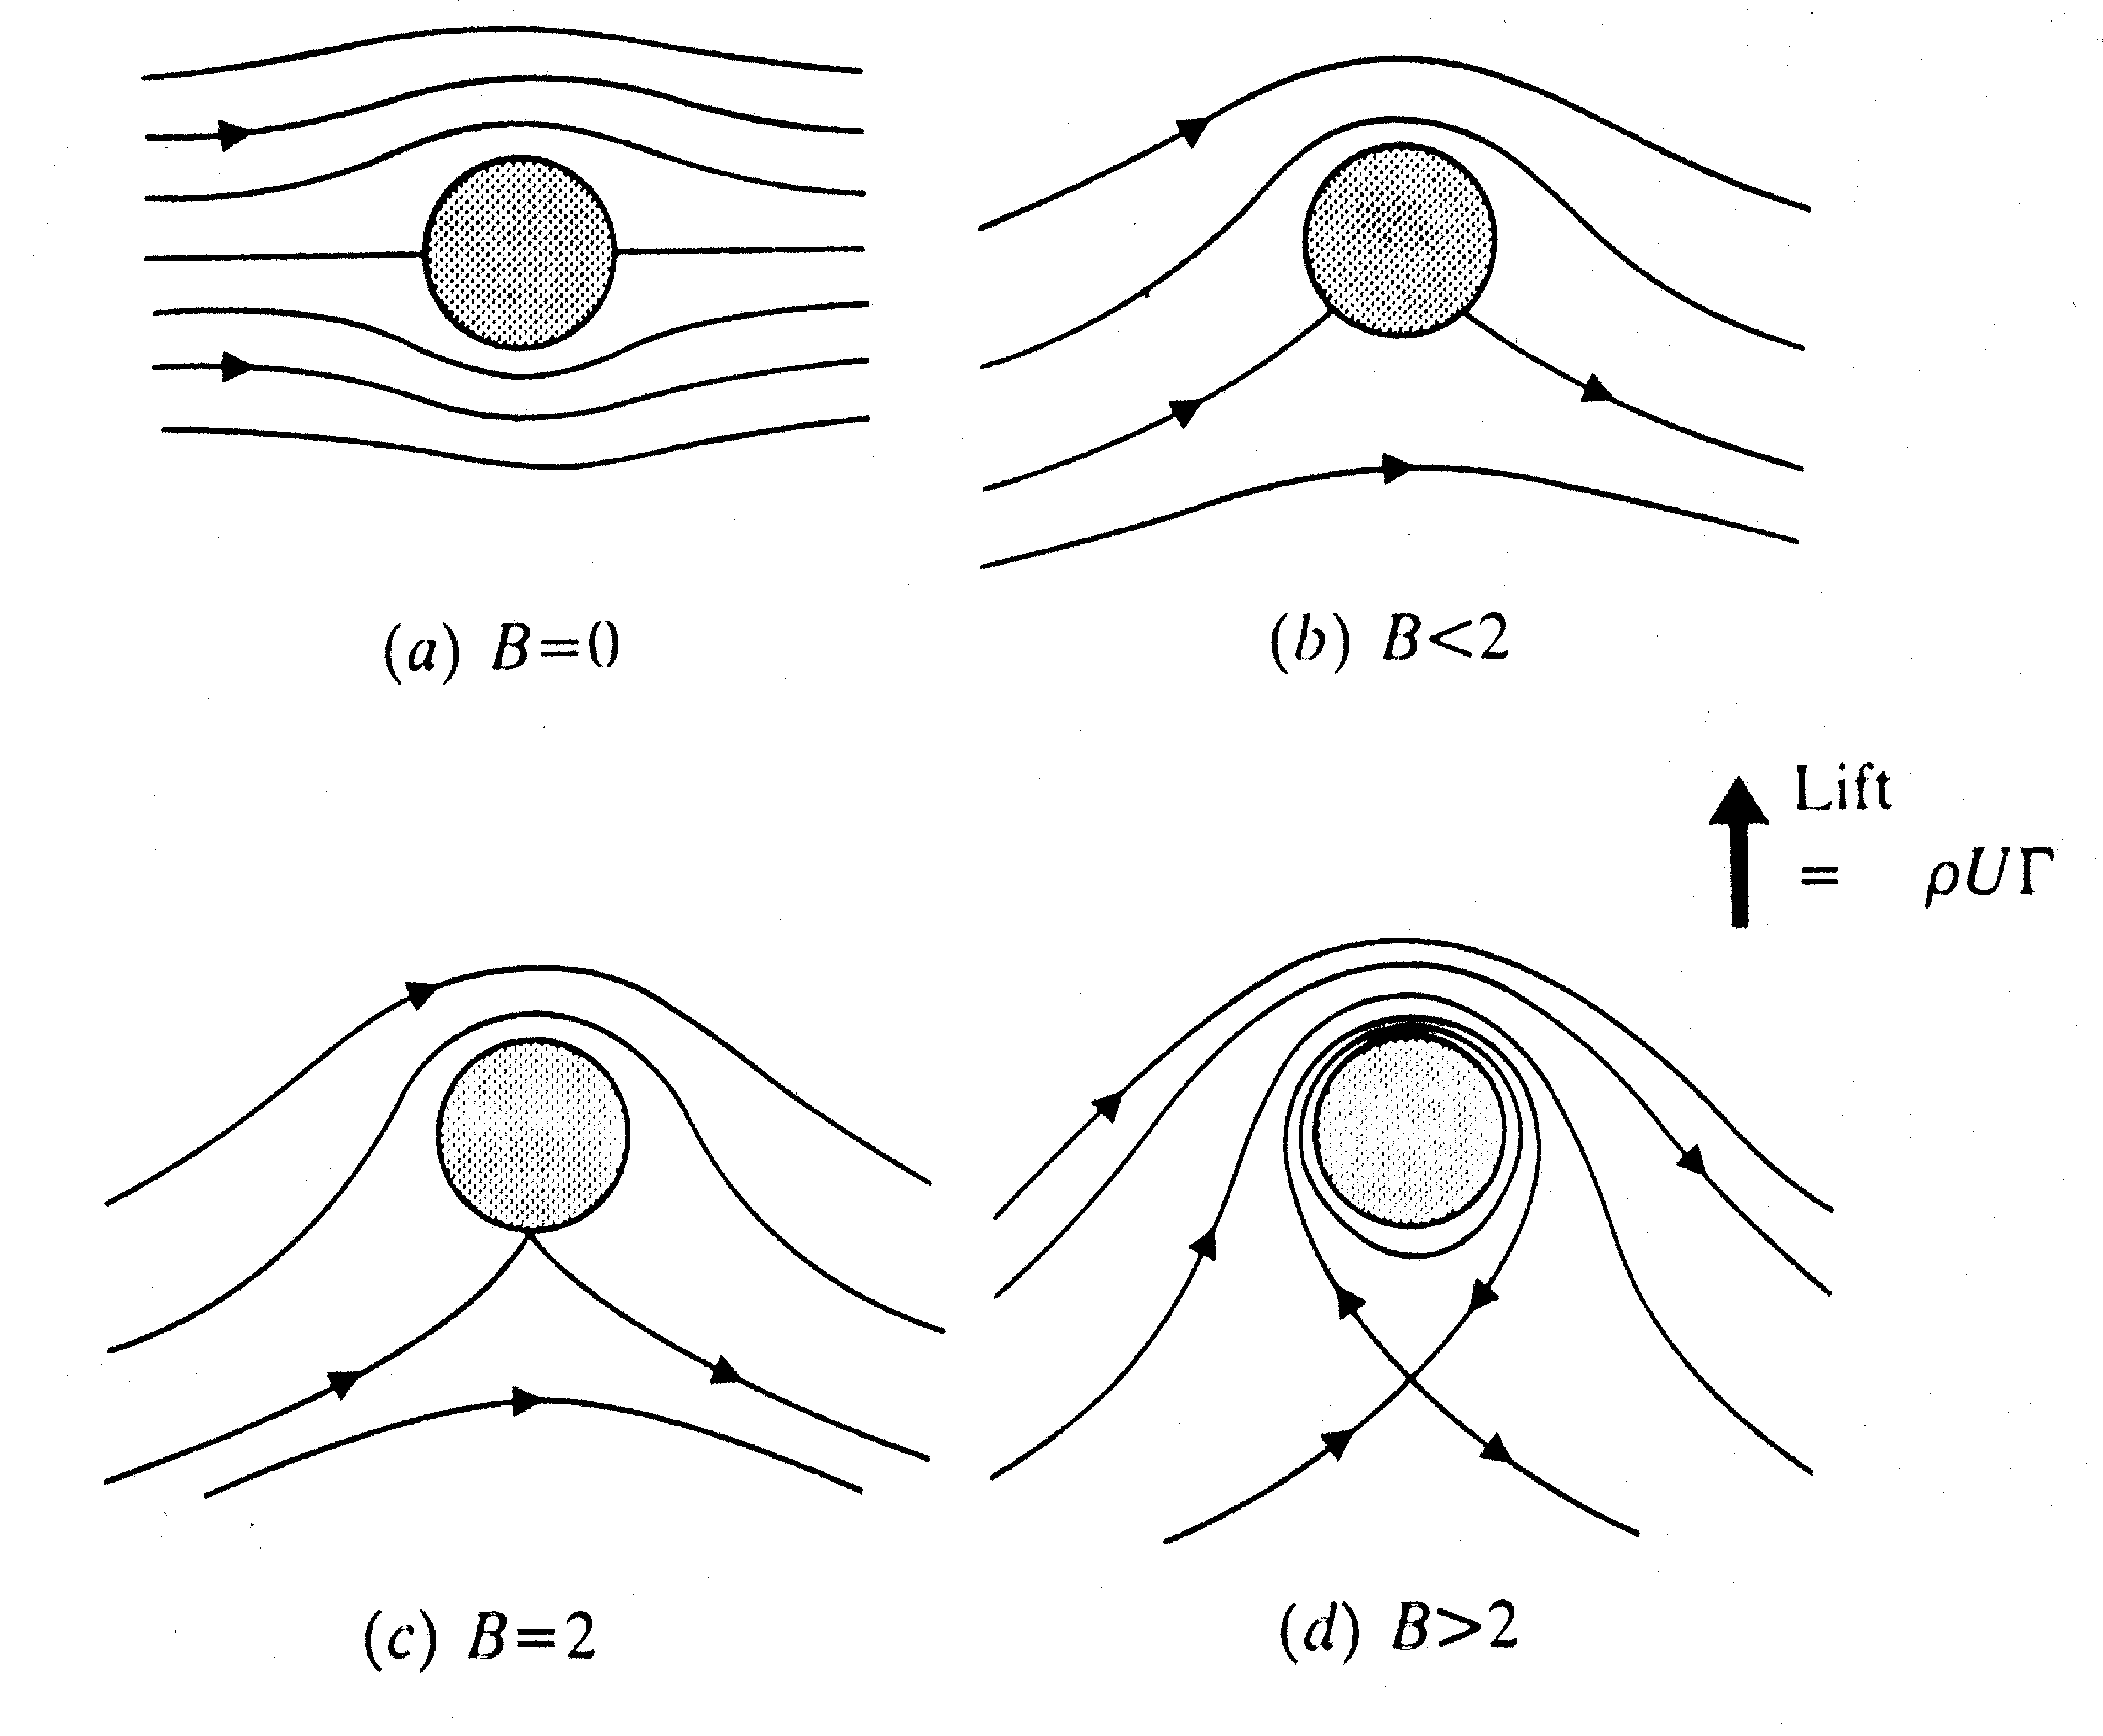
\includegraphics[width=4in]{Section77.pdf}}
{\small (From Elementary Fluid Dynamics. D.J. Acheson, 1990.)}
\label{fig7}
\end{figure}

As the surface of the cylinder is a streamline, Bernoulli's theorem requires 
that
\[
\frac{p}{\rho }+\frac{{{\bf u}}^2}{2}=\hbox{constant along } r=a.
\]
Therefore, 
\begin{align*}
\frac{p}{\rho } & = \hbox{constant}-\frac{v_\theta ^2 }{2}, \\
& =\hbox{constant} -\frac{1}{2}\left( {4U^2\sin ^2\theta +\frac{2U\kappa }{\pi 
a}+\frac{\kappa ^2}{4\pi ^2a^2}} \right), \\ 
& =\hbox{constant} -2U^2\sin ^2\theta -\frac{U\kappa }{\pi a}\sin \theta .
\end{align*}
The pressure thrust (per unit length in the $y$ direction) on a small element 
of the cylinder is $-\left( {pa} \right)d\theta $, from which the vertical 
component is $-\left( {pa\sin \theta } \right)d\theta $. 
It follows that the vertical component of the net thrust on the cylinder is
\begin{align*}
\hbox{Lift} = & \int_0^{2\pi } \rho \left( {2U^2\sin ^2\theta +\frac{U\kappa }{\pi 
a}\sin \theta -\hbox{constant}} \right)a\sin \theta d\theta , \\
& =\frac{\rho U\kappa }{\pi }\int_0^{2\pi } {\sin ^2\theta } d\theta  \\
& =\rho U\kappa.
\end{align*}

This is an example of the celebrated \textbf{Kutta-Joukowski lift theorem}. 
A similar calculation shows that the force in the direction of the stream, 
the \textbf{drag}, is zero. If the flow is irrotational, there is no drag on 
the body as the drag depends on the formation of a wake. This is, of course, 
an unrealistic feature of the solution. On the other hand, the body 
experiences \textbf{lift}, which is a force normal to the stream. The 
magnitude of the lift is $\rho U\kappa $ and is independent of the shape 
of the body (although the circulation depends on its shape). Physically, the 
addition of a clockwise (irrotational) swirling stream to that produced by 
uniform flow past the cylinder increases the velocity on the top of the 
cylinder and reduces it on the bottom. Bernoulli's theorem requires the 
pressure to decrease where the velocity increases and the pressure to 
increase where the velocity decreases. Consequently, the pressure field 
 produces a net transverse force on the 
cylinder toward increasing $z$. Circulation is the mechanism by which aircraft 
wings (as well as many other objects including golf and cricket balls) 
produce \textit{lift}. 

The circulation is zero around an aerofoil prior to the take-off of an 
aircraft (panel a). As the aircraft accelerates during take-off the aerofoil 
generates circulation in a thin boundary layer, which is subsequently 
advected into a thin wake. The thin wake \textit{rolls up}, producing what is known as a 
\textbf{starting vortex}. (You can generate similar vortices on each side of 
a spoon by drawing along through the surface of a cup of coffee.) As the 
circulation is zero at the initial time, it remains zero for all time by 
Kelvin's theorem, provided we take a contour large enough to enclose both 
the aerofoil and the starting vortex (panel b). Consequently, there must be 
circulation around the aerofoil which is equal and opposite of that in the 
wake (panel c). The circulation generated around the aerofoil generated this 
way provides the lift.

\begin{figure}
\begin{center}
\subfigure[]{\qquad \qquad \qquad \qquad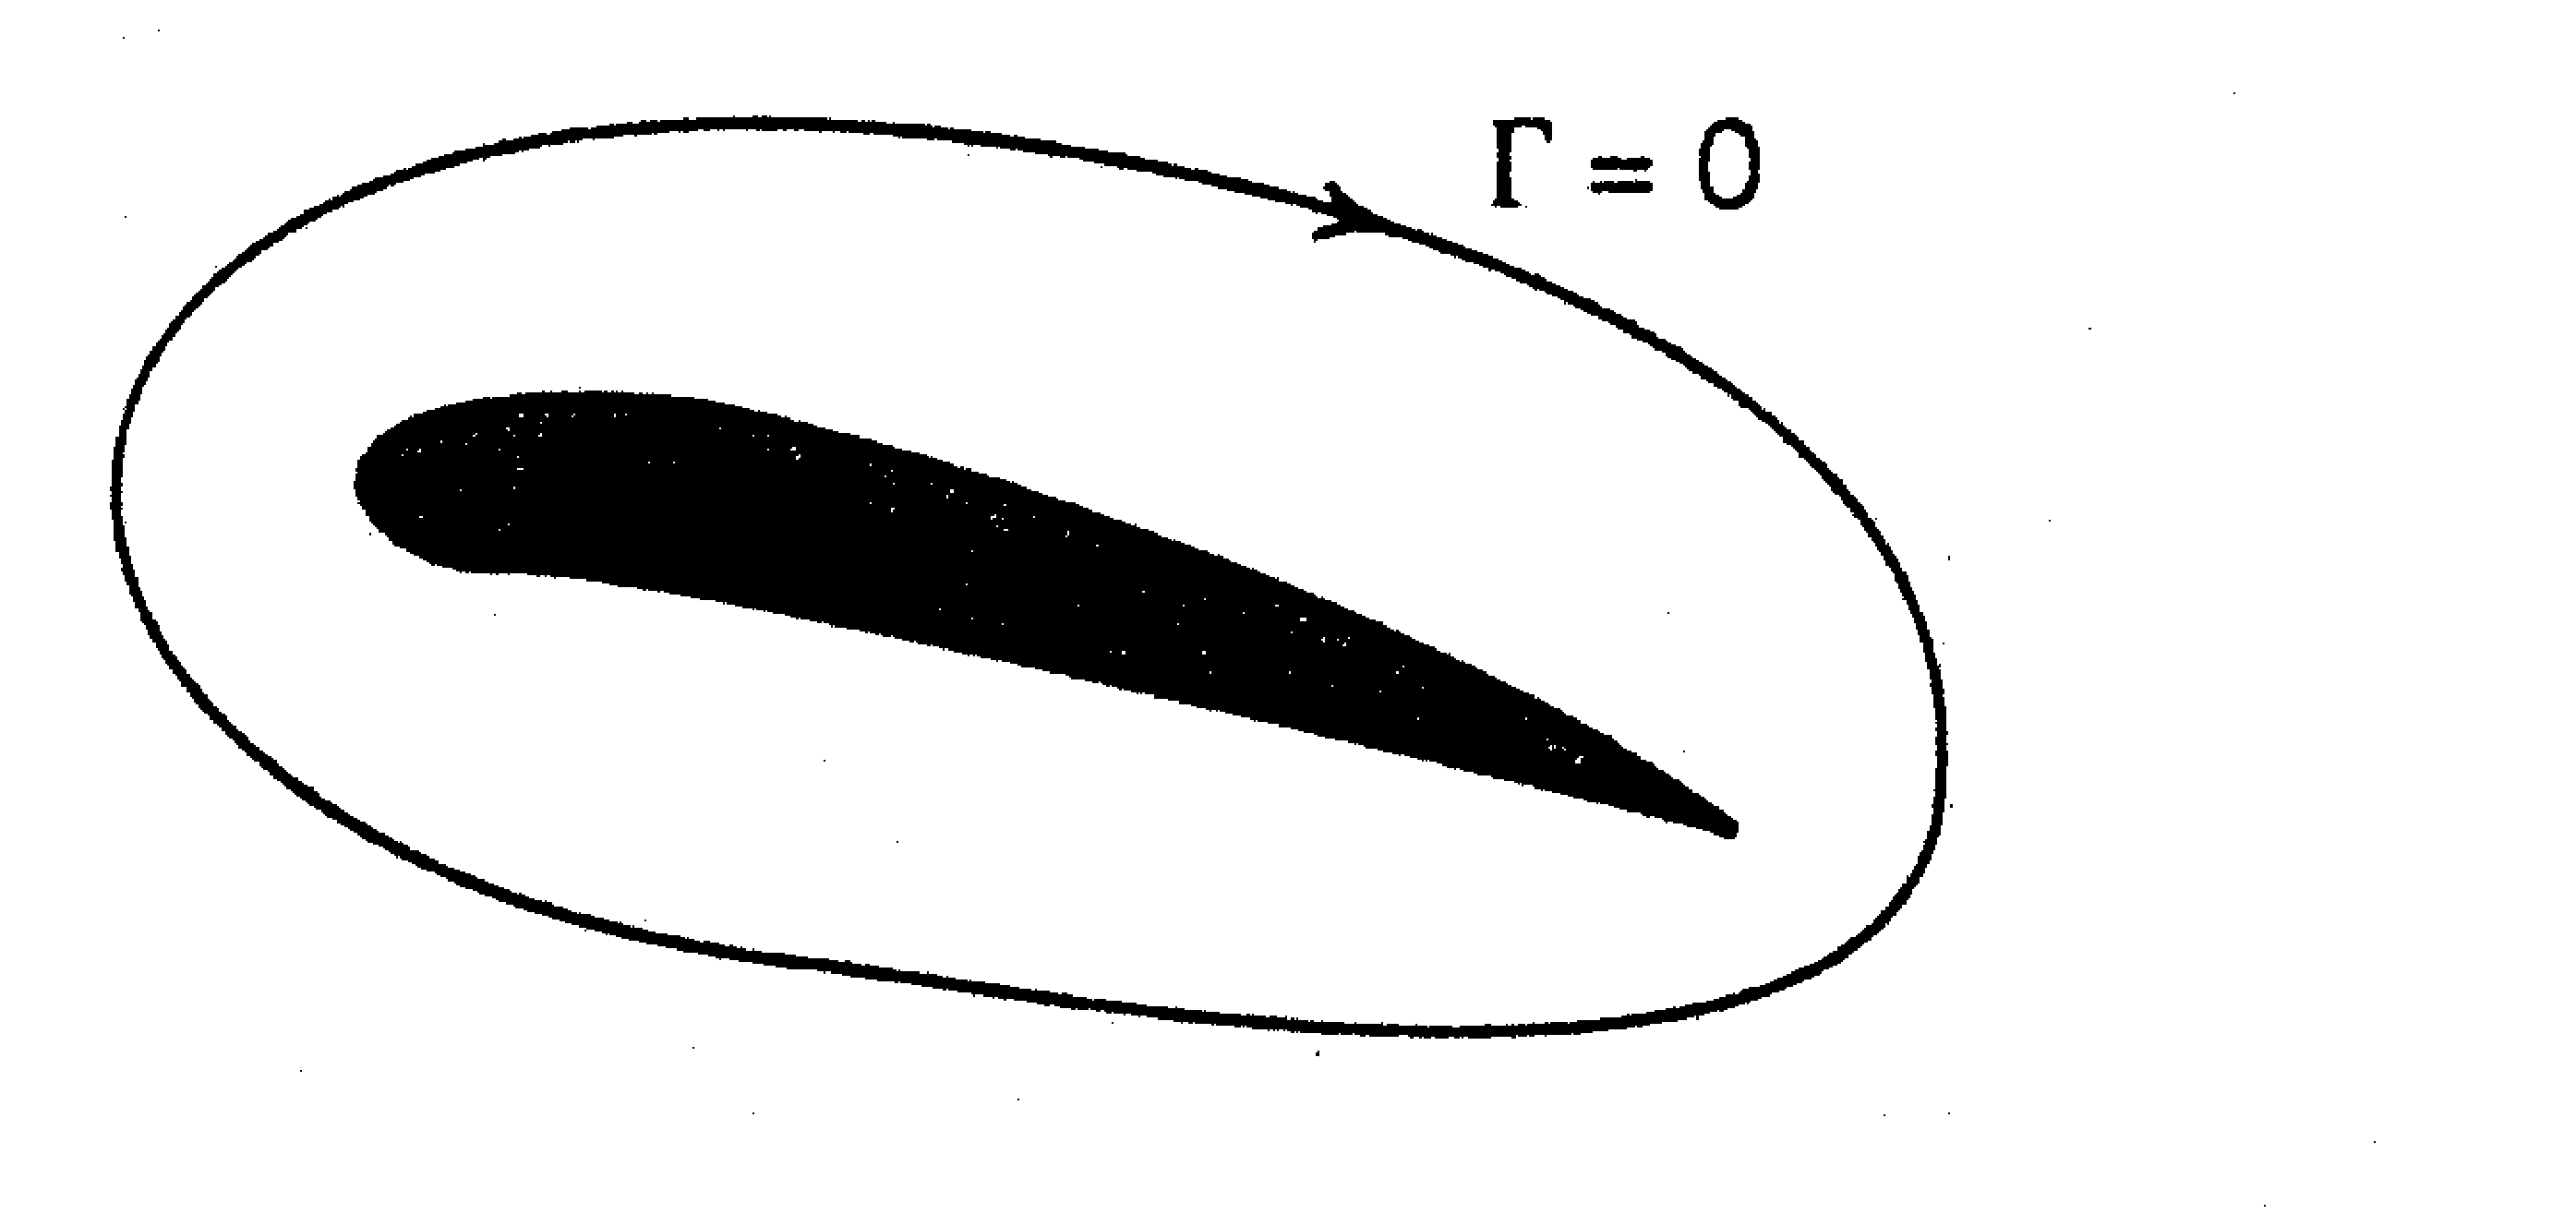
\includegraphics[width=3in]{Section78.pdf}}
\subfigure[]{\qquad \qquad \quad 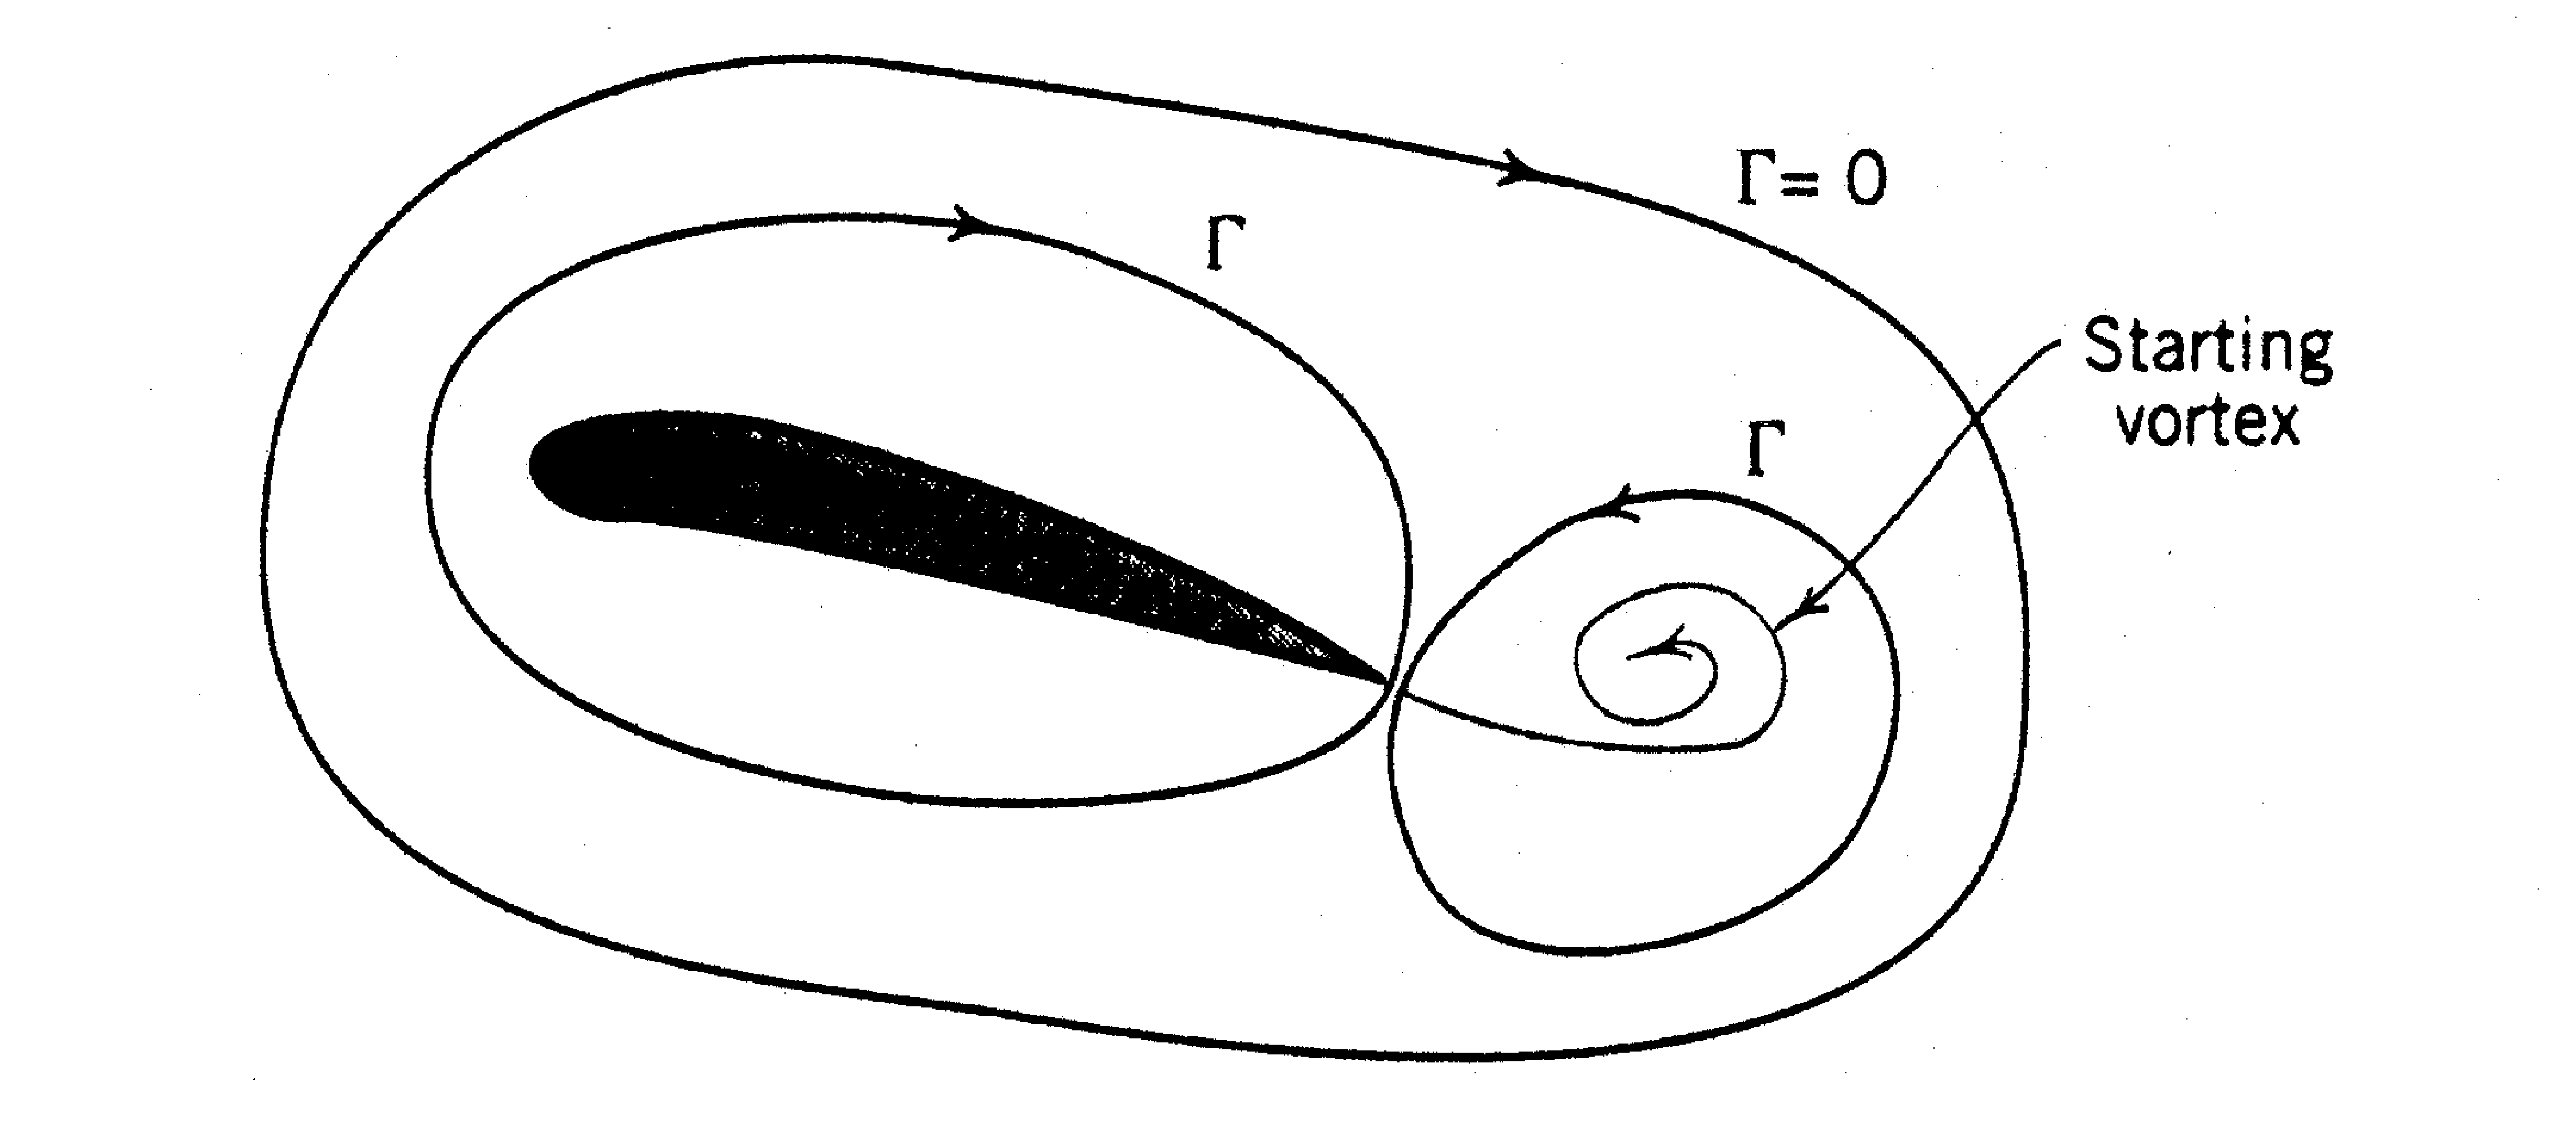
\includegraphics[width=4.25in]{Section79.pdf}}
\subfigure[]{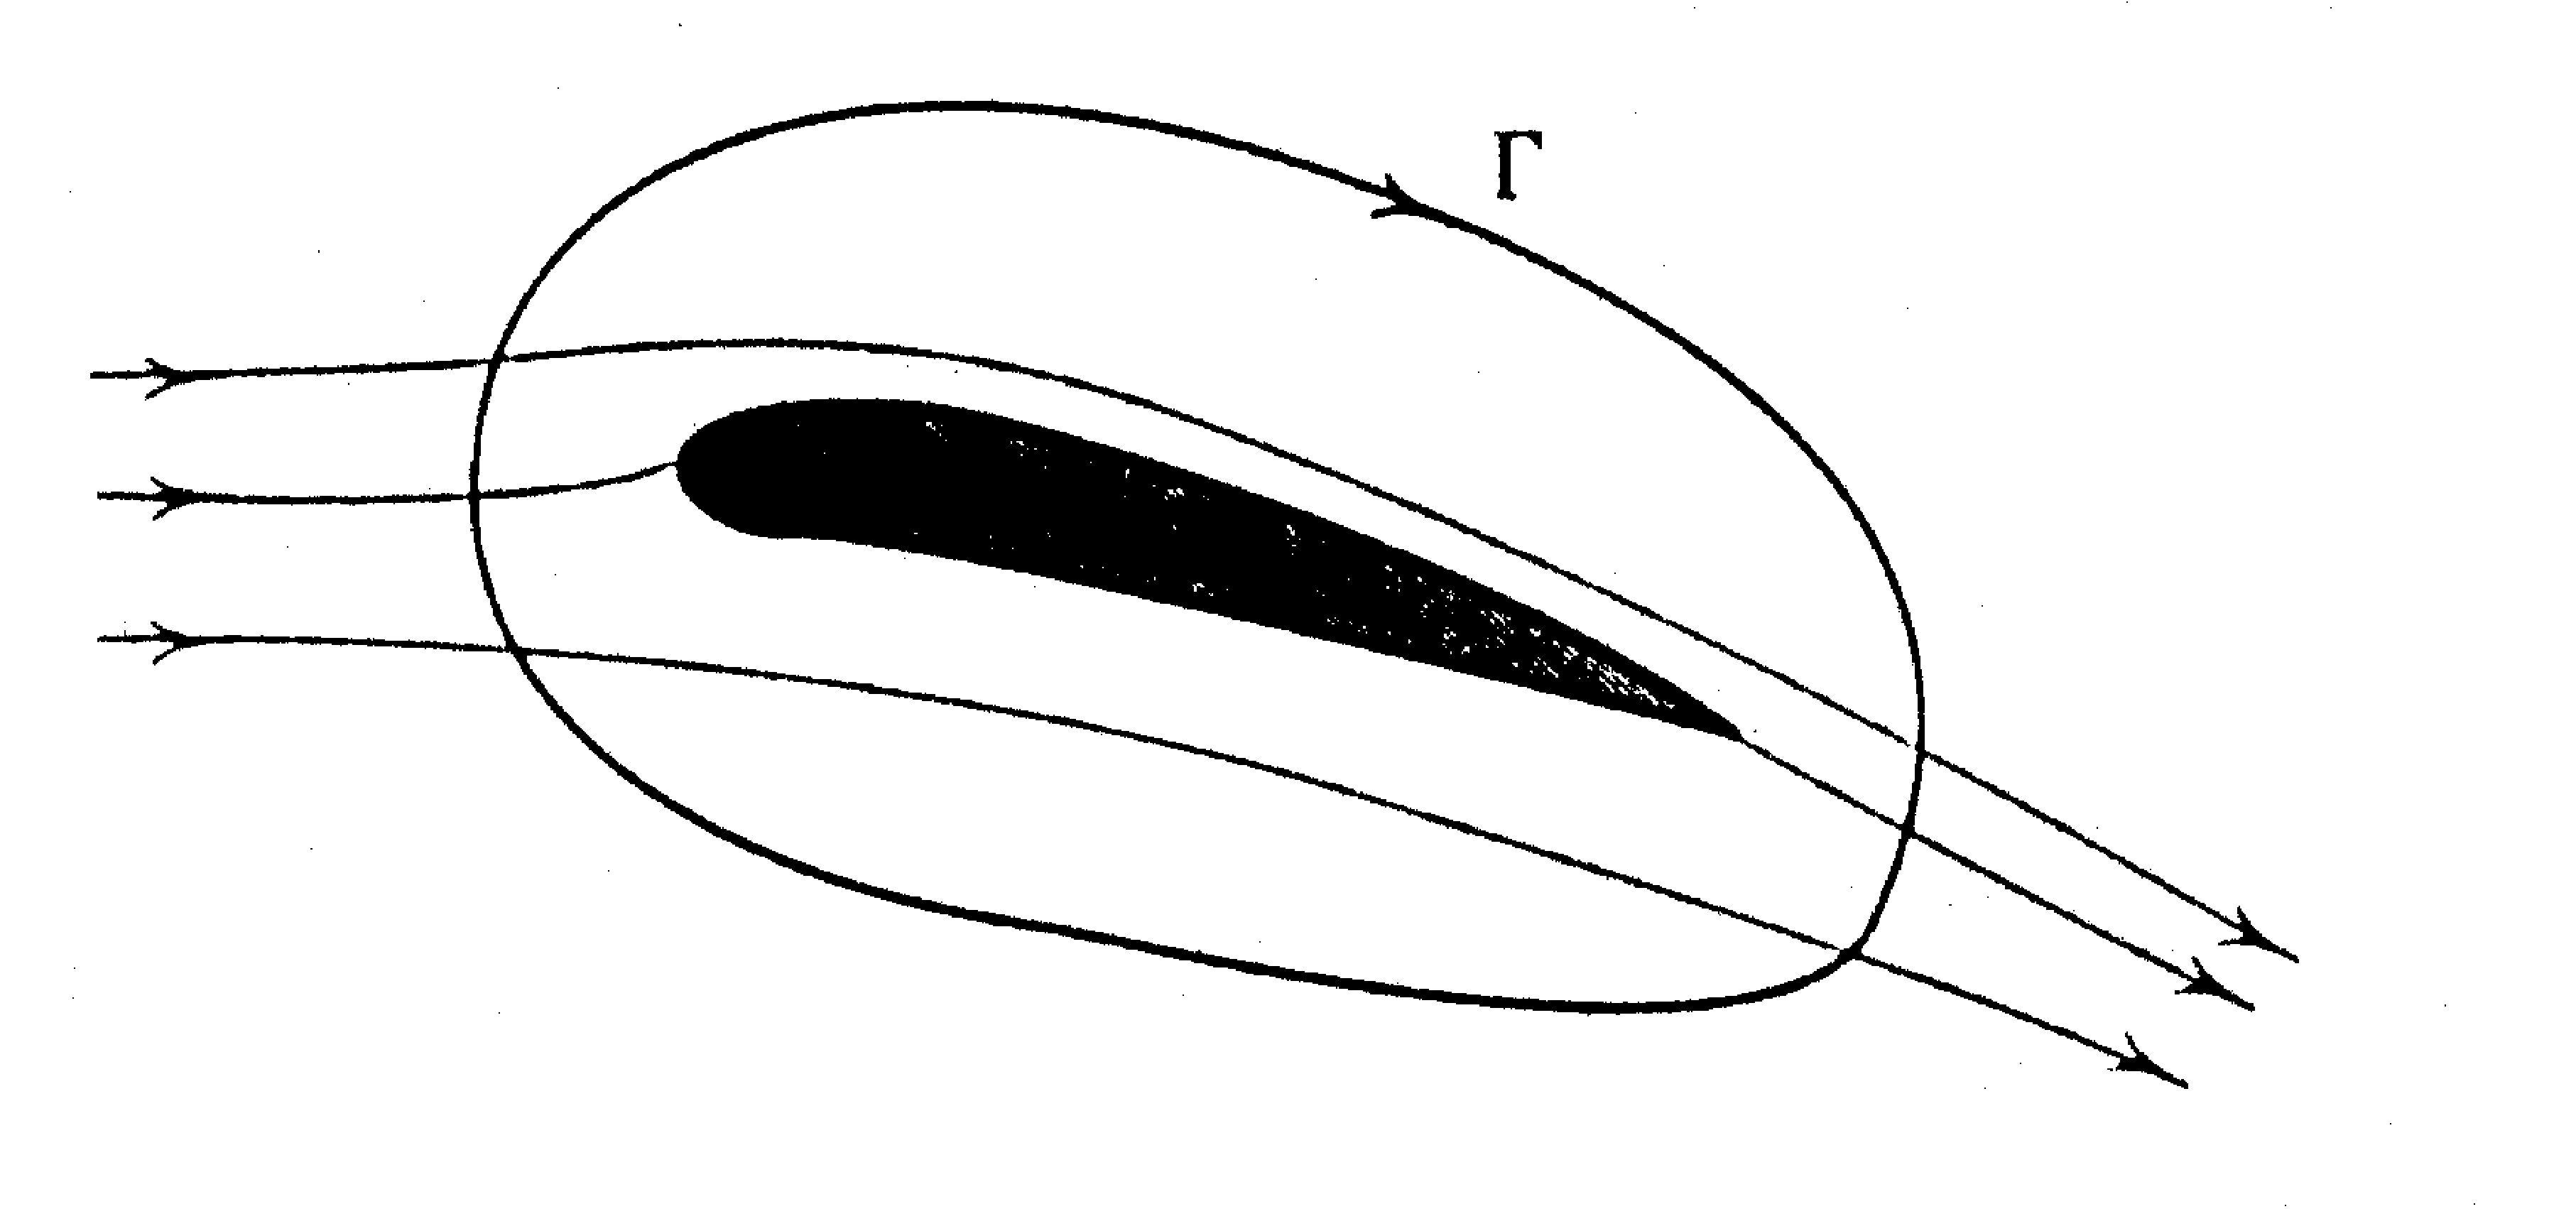
\includegraphics[width=4in]{Section710.pdf}\qquad \qquad }
\end{center}
\label{fig10}
\end{figure}

\subsection*{Exercises}

\begin{enumerate}
\item Show that $\left( {{{\bf u}}. \nabla } \right)\psi =0$ and hence 
the streamfunction is constant along a streamline.

\item Show that ${{\bf u}}=-\nabla \times \left( {\psi {{\bf j}}} 
\right)$.

\item Show that in cylindrical polar coordinates the radial and tangential 
components of velocity, $v_{r}$ and $v_{\theta }$, are related to the 
streamfunction by
\[ v_r =\frac{1}{r}\frac{\partial \psi }{\partial \theta } \quad\hbox{and}\quad v_\theta 
=-\frac{\partial \psi }{\partial r}. \]

\item  In rectangular cartesian coordinates, the two-dimensional form of 
Laplace's equation is 
\[ \frac{\partial ^2\psi }{\partial 
x^2}+\frac{\partial ^2\psi }{\partial z^2}=0. \]
 Show that in cylindrical 
polar coordinates Laplace's equation can be written
\[
\frac{1}{r}\left[ {\frac{\partial }{\partial x}\left( {r\frac{\partial 
\psi }{\partial r}} \right)+\frac{1}{r}\frac{\partial ^2\psi 
}{\partial \theta ^2}} \right]=0.
\]
\end{enumerate}


\end{document}
